
%%%%%%%%%%%% PREAMBLE %%%%%%%%%%%%%%%%%%%%%

% Initiate document
% -----------------
\documentclass[11pt,a4paper]{article}

% Document codification and language
\usepackage[utf8]{inputenc} % Codificação do documento (conversão automática dos acentos)
\usepackage[T1]{fontenc}
\usepackage[USenglish]{babel}

% Set up geometry of the document
\usepackage{geometry}
\geometry{a4paper,tmargin=2.54cm,bmargin=2.54cm,lmargin=2.54cm,rmargin=2.54cm}

% Load packages
% -------------
\usepackage[centertags]{amsmath}
\usepackage{amssymb}
\usepackage{amsthm}
\usepackage{amsfonts}
\usepackage{latexsym}
\usepackage{graphicx}

\usepackage{epstopdf} %converting to PDF
\usepackage{polynom}
\usepackage{verbatim}
\usepackage{rotating}

\usepackage{setspace}
\usepackage[section]{placeins}
\usepackage[justification=centering]{caption}
\usepackage{tabularx}
\usepackage{booktabs}
\usepackage{multirow}

\def\sym#1{\ifmmode^{#1}\else\(^{#1}\)\fi} %for \sym{*}

\usepackage{array}
\newcolumntype{C}{>{\centering\arraybackslash}m{2cm}}
\newcolumntype{D}{>{\centering\arraybackslash}m{1.81cm}}

\usepackage{color}
\setcounter{tocdepth}{4}
\usepackage{adjustbox}
\usepackage{pgfplots}
\usepackage{graphicx}
\usepackage{afterpage}
\usepackage{lscape}
%\usepackage{subfigure} is an obsolete package
\usepackage{subcaption} %is the new one
\usepackage[bottom]{footmisc}
\usepackage{longtable}
\usepackage{ragged2e}
\usepackage{pdflscape}
\usepackage{titlesec}

% HYPERLINKS
\usepackage[hyphens]{url}
\usepackage[backref]{hyperref}
\hypersetup{colorlinks=true,
            linkcolor=black,
            urlcolor=blue,
            citecolor=gray}

\renewcommand\backrefxxx[3]{%
    \hyperlink{page.#1}{\textcolor{red}{$\uparrow$#1}}%
    }

\usepackage{scalerel,stackengine}
\stackMath
\newcommand\reallywidehat[1]{%
    \savestack{\tmpbox}{\stretchto{%
        \scaleto{%
        	\scalerel*[\widthof{\ensuremath{#1}}]{\kern-.6pt\bigwedge\kern-.6pt}%
        	{\rule[-\textheight/2]{1ex}{\textheight}}%WIDTH-LIMITED BIG WEDGE
        	}{\textheight}% 
    	}{0.5ex}}%
    \stackon[1pt]{#1}{\tmpbox}%
}

\usepackage[round]{natbib}
\bibliographystyle{ecta}

\pgfplotsset{compat=1.14}
\begin{document}
	
	% Title page
	% ----------
	
	\font\myfont=cmr12 at 19pt
	\title{\myfont{Supporting Teacher Autonomy to Improve Education Outcomes: Experimental Evidence from Brazil}\thanks{This draft benefited from comments from Pablo Acosta, Guadalupe Bedoya, Paul Christian, Flavio Cunha, Steven Glover, John Loeser, Pedro Olinto, Ravi Somani, and seminar participants in São Paulo School of Economics (EESP-FGV). We thank the World Bank i2i fund and the World Bank Brazil Country Office for generous  research  funding. Finally, we thank the staff at the Rio Grande State Secretariat of Education for being great research partners. Computational reproducibility was verified by DIME Analytics. Details of the reproducibility checklist can be found in the \href{https://github.com/worldbank/brazil-pip-education/pip_app.pdf}{Online Appendix}. The reproducibility package is available on \href{https://github.com/worldbank/brazil-pip-education}{GitHub}. The views expressed in this manuscript do not reflect the views of the World Bank. All errors are our own.}}
	
	\newcommand*\samethanks[1][\value{footnote}]{\footnotemark[#1]}
	
	\author{%
		Caio Piza\thanks{Development Impact Evaluation (DIME), The World Bank, 1818 H Street NW, Washington, DC 20433, United States.}%
		\and Astrid Zwager\samethanks[2]%
		\and Rafael Dantas\samethanks[2]%
		\and Andre Loureiro\thanks{Education Global Practice, The World Bank.}%
		\and Matteo Ruzzante\samethanks[2]
	}
	
	
	\date{}
	
	\maketitle
	
	\begin{abstract}
		\setstretch{1.2}
		\noindent We present experimental evidence of an education project in Brazil that seeks to improve school quality by providing teachers with the tools to autonomously develop and implement a project aimed at engaging their students. The program was implemented by the state government in one of the worst performing states of the country and offered in Grades 5, 6 and 10. We find significant and consistent impacts of the program in 6\textsuperscript{th} grade, a critical year of transition from primary to lower-secondary education. We estimate impacts on learning of 0.15 SD and grade passing rates increased by 13\%. We show that the program reduced teacher turnover and positively impacted students' socio-emotional skills, suggesting improving teacher motivation and student-teacher interactions are potential mechanisms.   
	\end{abstract}
	
	
	\vspace{1.5em}
	\begin{flushleft}
		\textbf{Keywords:}  teacher autonomy, mentoring, school resources, complementarities, education policy, lower-secondary education.  \\[1em]
		\textbf{JEL Codes:} H52, I21, M52, O15 \\
	\end{flushleft}
	
	\newpage
	\sloppy
	
	% Set up paragraph
	\doublespacing
	
	\setlength\parskip{1em}
	\setlength\parindent{0pt}
	
	\titlespacing{\section}{0pt}{0.5\parskip}{*-0.75}
	\titlespacing{\subsection}{0pt}{0.5\parskip}{*-0.75}
	\titlespacing{\subsubsection}{0pt}{0.5\parskip}{*-0.75}
	
	%%%%%%%%%%%%%%%%% INTRODUCTION %%%%%%%%%%%%%%%%%%%%%%%%%
	
	\section{Introduction} \label{intro}
	
	%%% PARA 1: Quality of education matters for growth and equality
	
	Over the last three decades many countries succeeded in putting kids in school, but gains in learning have been limited \citep{WDR2018}. Improving quality of education and learning outcomes is a priority for many countries given its role in building human capital, affecting individual earning prospects and long-term growth (\citealp{hanushek2008role, hanushek2012better}; \citealp{chetty2014measuringII}). Despite increasing resource allocation to the sector, governments have struggled to substantially improve school quality (\citealp{mcewan2015improving}; \citealp{WDR2018}). The recent World Development Report points to a `learning crisis' faced by many countries, including Brazil, and the urgent need for solutions \citep{WDR2018}. 
	
	%%% Para 2: Teacher focus and motivation
	
	Many policies that seek to affect school outcomes focus on improving teacher qualification and motivation, as teachers are one of the main inputs in the education production function (\citealp{hanushek2008role}; \citealp{chetty2014measuringI, chetty2014measuringII}). While increasing teacher salary has been shown to have limited impact on student learning \citep{de2018double}, performance-based payments designed to align teacher incentives with the effective use of resources have yielded positive results in some contexts (\citealp{muralidharan2011teacher}; \citealp{duflo2012incentives}; \citealp{de2018double}; \citealp{mbiti2019inputs}). While theory predicts that incentive schemes, monetary or non-monetary, can have limited effect or even backfire if they crowd out intrinsic motivation \citep{benabou2006incentives}, empirical evidence suggests that non-monetary incentives can complement intrinsic motivation at least in some contexts (\citealp{bowles2012economic}; \citealp{ashraf2014no}).
	
	%%% Para 3: Complementarities 
	
	Recent evidence suggests that policies addressing multiple constraints through complementary interventions are more likely to deliver larger impacts on learning outcomes. In a recent paper, \cite{mbiti2019inputs} find large impacts on learning only when tackling multiple barriers simultaneously, such as inadequate school resources and low teacher motivation. They find large impacts on learning only in schools that received both grants and teacher incentives. Along similar lines, \cite{andrew2019preschool} find that substantial increases in per student spending are ineffective unless combined with complementary resources such as pedagogical training and coaching.
	
	%%% Para 4: Autonomy and intrinsic vs extrinsic motivation
	
	In this paper we study whether autonomy combined with technical support can crowd in intrinsic motivation of local implementers, such as teachers, in a low capacity context. The effect of assigning local implementers with more autonomy on the quality of public service provision is an empirical question. On the one hand, increasing local autonomy may encourage agents (local implementers) to reduce effort due to reduced ability of central government to observe and reward effort accordingly. On the other hand, greater autonomy can improve service delivery by providing a non-monetary incentive for local implementers and by leveraging their superior local knowledge \citep{rogger2018hierarchy}. \cite{rasul2018management} find that more autonomy can improve the quality of public projects delivered even in contexts of low government capacity. These results have direct implications for policy design in countries that might neither have fiscal space to design pay-for-performance schemes at scale nor effective monitoring mechanisms. 
	
	%%% Para 5: Introduction of what we study in what context
	
	We present experimental evidence of an education policy in Brazil that seeks to improve school quality by providing teachers with the tools to autonomously develop and implement a project aimed at engaging their students. The initiative is called the Pedagogical Innovation Project (\textit{Projeto de Inovação Pedagógica} -- PIP) and was implemented by the State Secretariat of Education (SEE) of Rio Grande do Norte (RN) with the objective to improve both student progression and learning outcomes in primary and secondary schools. RN is one of poorest states in the country and consistently scores at the bottom of the Brazilian Education Development Index, \textit{Indice de Qualidade da Educação Básica} (IDEB). 
	
	%%% Para 6: Description of the project
	
	The PIP provided teacher with the autonomy to design and implement a local project to tackle their specific issues instead of prescribing ``solutions''. The autonomy was combined with substantial technical assistance that focused on general concepts of project design, planning and implementation as well as a small grant. Through seminars and the support from a dedicated mentor, schools developed a diagnostic of their main pedagogical challenges and a context-specific project to address them. Mentors supported teachers to develop innovative projects that include interdisciplinary elements and explore other forms of teaching beyond traditional lecture style, as well as highlighting the importance of pedagogical planning. The decentralized approach sought to ensure relevance of the interventions as well as motivate teachers by giving them the autonomy over design and implementation. Throughout the academic year the mentors worked with the teachers to help plan activities and resolve implementation bottlenecks. As such, mentors complemented local capacity while ensuring close ties with central government, possibly reducing moral hazard concerns associated with strategic behavior of local staff. Approved proposals were awarded financial support from the SEE to implement the projects, ranging from about US\$ 7,500 to US\$ 11,000.\footnote{30,000 to 45,000 Brazilian Reais, using exchange rate on 12/31/2015.}
	
	% Describe the experiment and data
	
	The PIP was launched in 2014 and covered a total of 397 of the 639 state schools across the 2015 to 2018 academic years. We focus on the 2016 edition, which targeted the final grade of primary education (5\textsuperscript{th} grade), the first grade of lower secondary education (6\textsuperscript{th} grade) and the first grade of upper secondary education (10\textsuperscript{th} grade), with the latter two generally being the most problematic in terms of repetition and dropout rates. The 126 schools that participated that year were randomly selected among the 299 schools eligible to receive the project in 2016 and covered approximately 9500 students. 
	
	% Present main results - learning and progression
	
	We first show that the project had substantial impacts on both learning and progression for 6\textsuperscript{th} grade students, a critical grade in school transition from primary to lower-secondary education \citep{dos2017mais}. Our ITT estimates point to an impact of 0.18 SD on math and 0.16 SD in Portuguese. We estimate the average impact on learning to be the equivalent to 0.5 extra year of schooling. Consistent with the results on learning gains, we find substantial improvements in grade 6 passing rates, which are estimated to increase by 8.5 percentage points (pp), a 13\% improvement compared to the control mean.
	
	% Mechanisms
	
	We hypothesize two main channels through which the program may impact learning and grade progression: (1) increasing teacher motivation and (2) implementation of innovative projects. These may in turn both affect student-teacher interactions. Teacher autonomy over the design and use of the grant likely affects student outcomes through both channels: it may crowd in teacher intrinsic motivation and affect teaching quality as well as lead to better designed projects. The technical assistance works mainly through the second channel. We cannot tell apart the relative importance of these two main intervention components as the same package was offered to all treatment schools. However we do investigate which channels were likely affected and potential complementarities between the two.  
	
	% Results on mechanisms
	
	To assess the first mechanism, we use teacher turnover as a proxy of teacher motivation. We estimate that the PIP reduced teacher turnover in Grade 6 by 9.3\% over the control mean, which we interpret as a positive impact on teacher motivation. Although our design does not allow us to isolate the second channel, we leverage the fact that most Grade 6 teachers also teach Grade 7 to shed light on whether shifting teacher motivation is sufficient. We estimate a similar reduction on 7\textsuperscript{th} grade teacher turnover, yet do not find impacts on passing rates, repetition and/or dropout rates of 7\textsuperscript{th} grade students. These results provide suggestive evidence that the PIP approach led to more commitment from teachers, but this alone was not sufficient to affect grades that did not also have the innovative projects implemented. To corroborate whether affecting teacher turnover is likely to impact final outcomes, we estimate heterogeneous effects by teacher turnover at baseline. We find that schools with higher teacher turnover at baseline are driving the impacts both on teacher turnover and learning. Impacts of the program on learning in schools with high teacher turnover at baseline approach 0.28 SD. 
	
	Both hypothesized channels may improve student-teacher interaction, which are expected to impact students' socio-emotional skills as a result. We measured the Big Five personality traits and find positive impacts on conscientiousness and extroversion for 6\textsuperscript{th} graders. Conscientiousness is the trait most commonly associated with the acquisition of cognitive skills (\citealp{poropat2009meta}; \citealp{ivcevic2014predicting}). 
	
	Taken together, our results suggest that the program was particularly successful in grade 6. Grade 6 is a critical moment for students as they transition from primary to lower-secondary education. During this transition, students move from having a single teacher to multiple teachers resulting in weaker ties between students and teachers which has been shown to affect learning (\citealp{bedard2005middle}; \citealp{hanewald2013transition}; \citealp{dos2017mais}). Improving teacher motivation and student-teacher interactions, may therefore be particularly effective at this stage. Teachers from Grade 6 may have perceived the approach to be relevant to overcome their particular challenges, which may explain why implementation in this grade was better than in the other grades.    
	
	% Contributions
	
	Our paper contributes to several strands of the literature. First, it provides experimental evidence that stimulating autonomy of local civil service providers, such as teachers, can improve outcomes even in a low capacity environment. Second, our results suggest that efficiency gains can be obtained in public schools, as improved education outcomes were achieved to a large extent leveraging existing resources. This is consistent with the increasing body of evidence pointing to the importance of school management in improving educational outcomes through better resource allocation (\citealp{abdulkadirouglu2011accountability}; \citealp{dobbie2013getting}; \citealp{rockoff2012information}: \citealp{taylor2012effect}; \citealp{fryer2014injecting}; \citealp{fryer2017management}). Finally, our results suggest that increasing teacher motivation alone is unlikely to produce similar results on learning and progression, reinforcing the view that complementarities matter (\citealp{WDR2018}; \citealp{gilligan2018educator}; \citealp{andrew2019preschool}; \citealp{mbiti2019inputs}). This is in line with results from two non-experimental evaluations of another education policy in Brazil, called  Mais Educação, which showed that providing teachers with the autonomy over some resources, without technical assistance had limited results (\citealp{almeida2016assessing}; \citealp{de2016impacto}). Taken together, the results suggest that the strength of the project was in combining the provision of autonomy with the means to implement an innovative project, with substantial technical assistance.  
	
	% Organization of the paper
	
	The remainder of the paper is organized as follows. Section \ref{sec:context} details the intervention. Section \ref{sec:design_data} describes the experimental design and data sources. Section \ref{sec:methodology_results} presents the empirical strategy and results, while Section \ref{sec:mechanism} explores potential mechanisms driving the main impacts. Section \ref{sec:policy} provides back-of-the-envelope estimates for the impact of the program on school quality indicators and individuals' expected earnings. Section \ref{sec:conclude} concludes with policy recommendations.
	
	%%%%%%%%%%%%%%%%%%%% CONTEXT %%%%%%%%%%%%%%%%%%%%%%%%%%
	
	\section{Context and Intervention} \label{sec:context}
	
	\subsection{Education in Brazil and Rio Grande do Norte} \label{sec:brazil}
	
	In the last few decades, Brazil has made significant progress to guarantee universal access to primary education, reaching a 99\% enrollment rate for children between the age of 6 and 14 years in 2018.\footnote{Source: National Household Survey (\textit{PNAD Contínua} and School Census).} Several factors contributed to this trend, including the establishment of a national education financing framework that increased spending per student in the poorest areas, as well as the conditional cash transfer program, \textit{Bolsa Família}, which requires families to enroll their children in school to receive the transfer \citep{glewwe2012impact}. 
	
	Brazil has the largest expenditure on education as share of GDP among developing countries, spending more than the average OECD country in relative terms.\footnote{See \url{https://data.oecd.org/eduresource/public-spending-on-education.htm} (last access: 07/16/2019). Source: ``Education at a glance: Educational finance indicators''.} Yet, significant challenges remain to keep kids in school and ensure quality of education. Grade repetition and dropout rates in primary and secondary schools are among the highest in the world. Large age-grade distortions are found across all grades and an average student spends 15 years -- instead of 12 -- to graduate from high school. Retention rates are particularly high in the 4\textsuperscript{th}, 5\textsuperscript{th}, 6\textsuperscript{th} and 10\textsuperscript{th} grades, where they range from 15\% to 30\% (Figure \ref{fig:grade_comparison_retention}). High school graduation rate is only 65\%.\footnote{Source: National Household Survey (\textit{PNAD Contínua} and School Census).} Despite the largest improvements in math score in the PISA evaluation between 2003 and 2012, Brazil still ranks below all LAC countries except for Peru and the Dominican Republic.\footnote{See \url{http://pisadataexplorer.oecd.org/ide/idepisa} (last access: 08/14/2019). Source: ``PISA Data Explorer''.} The 2018 World Development Report presented an alarming statistic for Brazil: at its current rate of improvement, it would take 260 years to reach OECD levels of reading \citep{WDR2018}. 
	
	These national figures hide a high degree of regional variation. In this paper we study an education project implemented by the Rio Grande do Norte (RN) state government, one of Brazil's poorest states. Results from the 2015 national standardized exam (\textit{Sistema de Avaliação da Educação Básica} -- SAEB) put RN state schools at the bottom of the learning distribution in both primary and lower secondary education. The test scores in SAEB indicate that only 39\% of 5\textsuperscript{th} graders and 24\% of 9\textsuperscript{th} graders achieved adequate reading levels for their grade. In math, the statistics are even more alarming with only 25\% and 9\% of 5\textsuperscript{th} grade and 9\textsuperscript{th} grade students reaching the expected proficiency levels for their grade.\footnote{Source: INEP.} The low level of learning is reflected in the state's progression indicators. In 2015\footnote{2015 is the year prior to the roll-out of the interventions we study in this paper.}, average school dropout at upper secondary education was 12.4\% compared to the national average of 8.8\% (Figure \ref{fig:grade_comparison_dropout}). The combination of high dropout rates and low learning outcomes put RN state schools near the bottom of the Brazilian quality of education index, the \textit{IDEB}\footnote{IDEB is a national indicator for the quality of education and combines information on student test scores and passing rates. IDEB was established in 2007 and it became one of the principal outcomes for Brazilian educational policy, setting targets for schools, municipalities and states.} (Figure \ref{fig:IDEB_byState}).
	
	% Dropout and retention rate in RN
	\begin{figure}[ht!]
		\caption{Grade Repetition and School Dropout Rates by Grade in Rio Grande do Norte}
		\label{fig:grade_comparison}
		
		\centering
		\captionsetup[subfigure]{position=top,justification=centering}
		
		\vspace{12pt}
		
		\begin{subfigure}{\textwidth}
			\centering
			\caption{Grade Repetition Rate}
			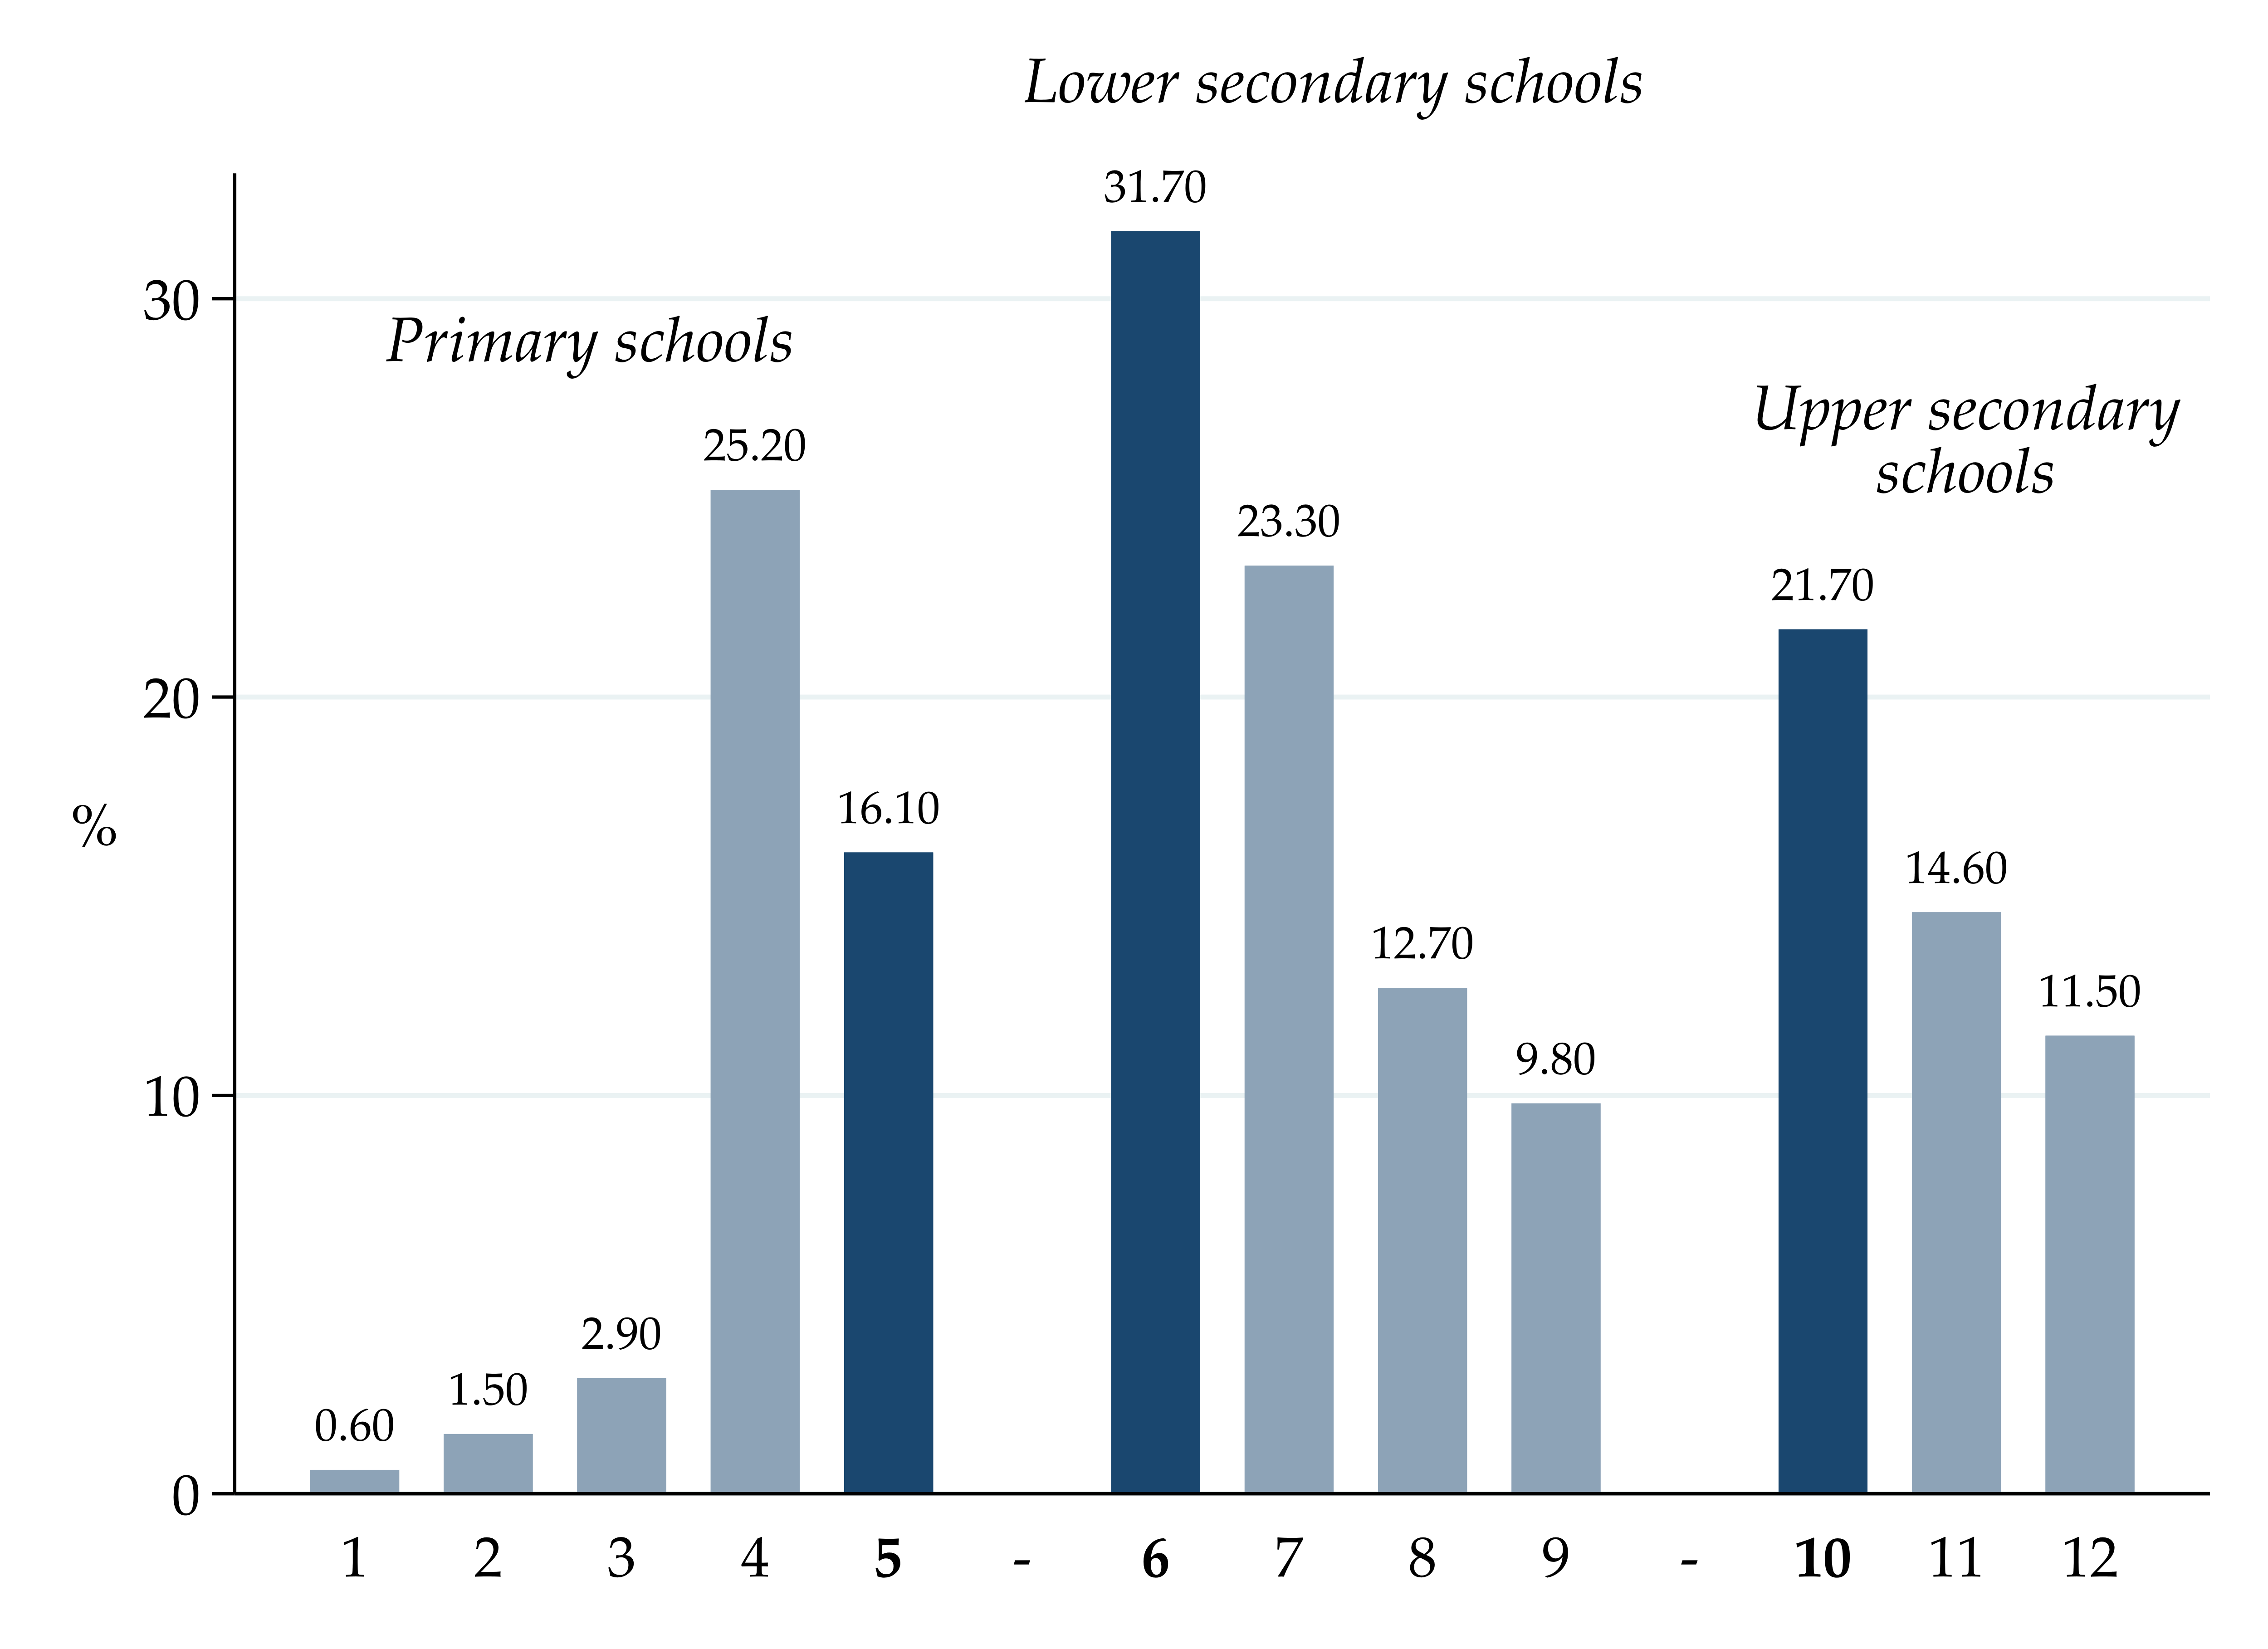
\includegraphics[width=13cm]{DataWork/Output/Figures/fig1a-grade_comparison_retention.png}
			\label{fig:grade_comparison_retention}
		\end{subfigure}
		
		\vspace{12pt}
		
		\begin{subfigure}{\textwidth}
			\centering
			\caption{School Dropout Rate}
			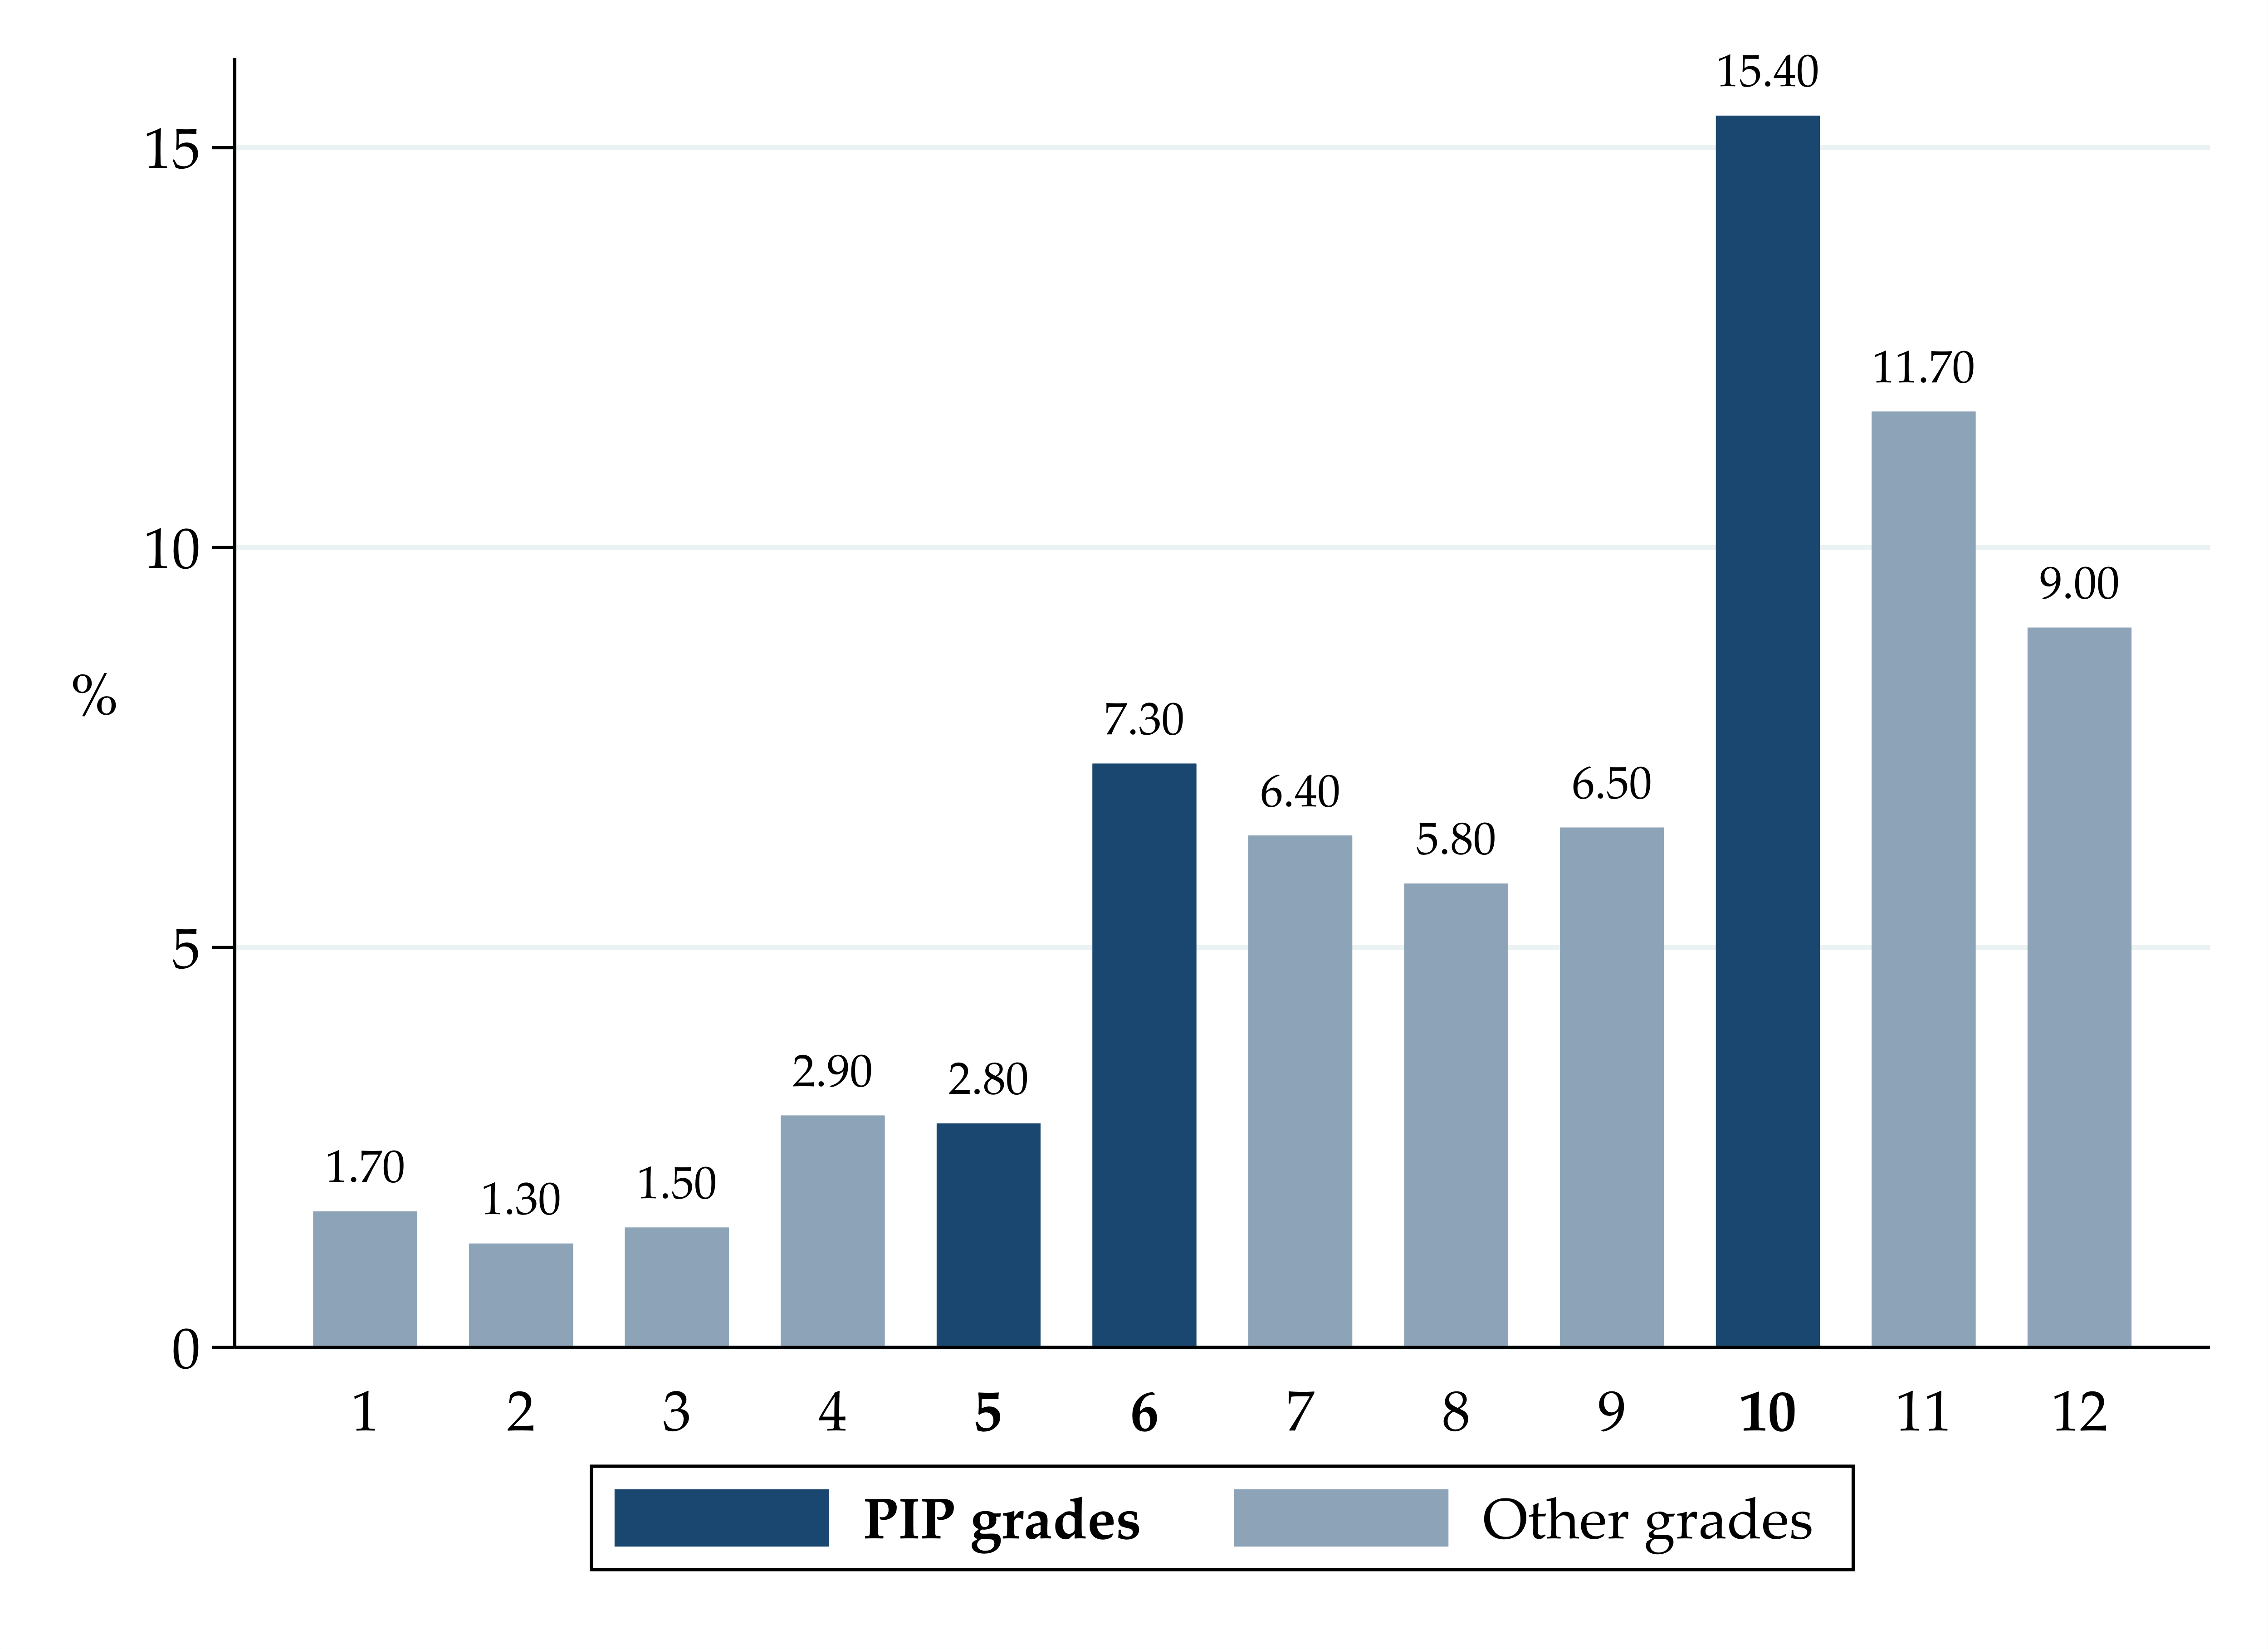
\includegraphics[width=13cm]{DataWork/Output/Figures/fig1b-grade_comparison_dropout.png}
			\label{fig:grade_comparison_dropout}  
		\end{subfigure}
		
		\begin{minipage}{0.8\textwidth}
			\small{\textit{Notes:} The bars show average retention and dropout rate among public schools in Rio Grande do Norte in 2015. Data are from \textit{Instituto Nacional de Estudos e Pesquisas Educacionais Anísio Teixeira} (INEP).}
		\end{minipage}
	\end{figure}
	%
	
	% IDEB RN vs. other Brazilian states
	\begin{figure}[ht!]
		\caption{IDEB in Rio Grande do Norte vs.\ Other Brazilian States, 2015}
		\label{fig:IDEB_byState}
		\centering
		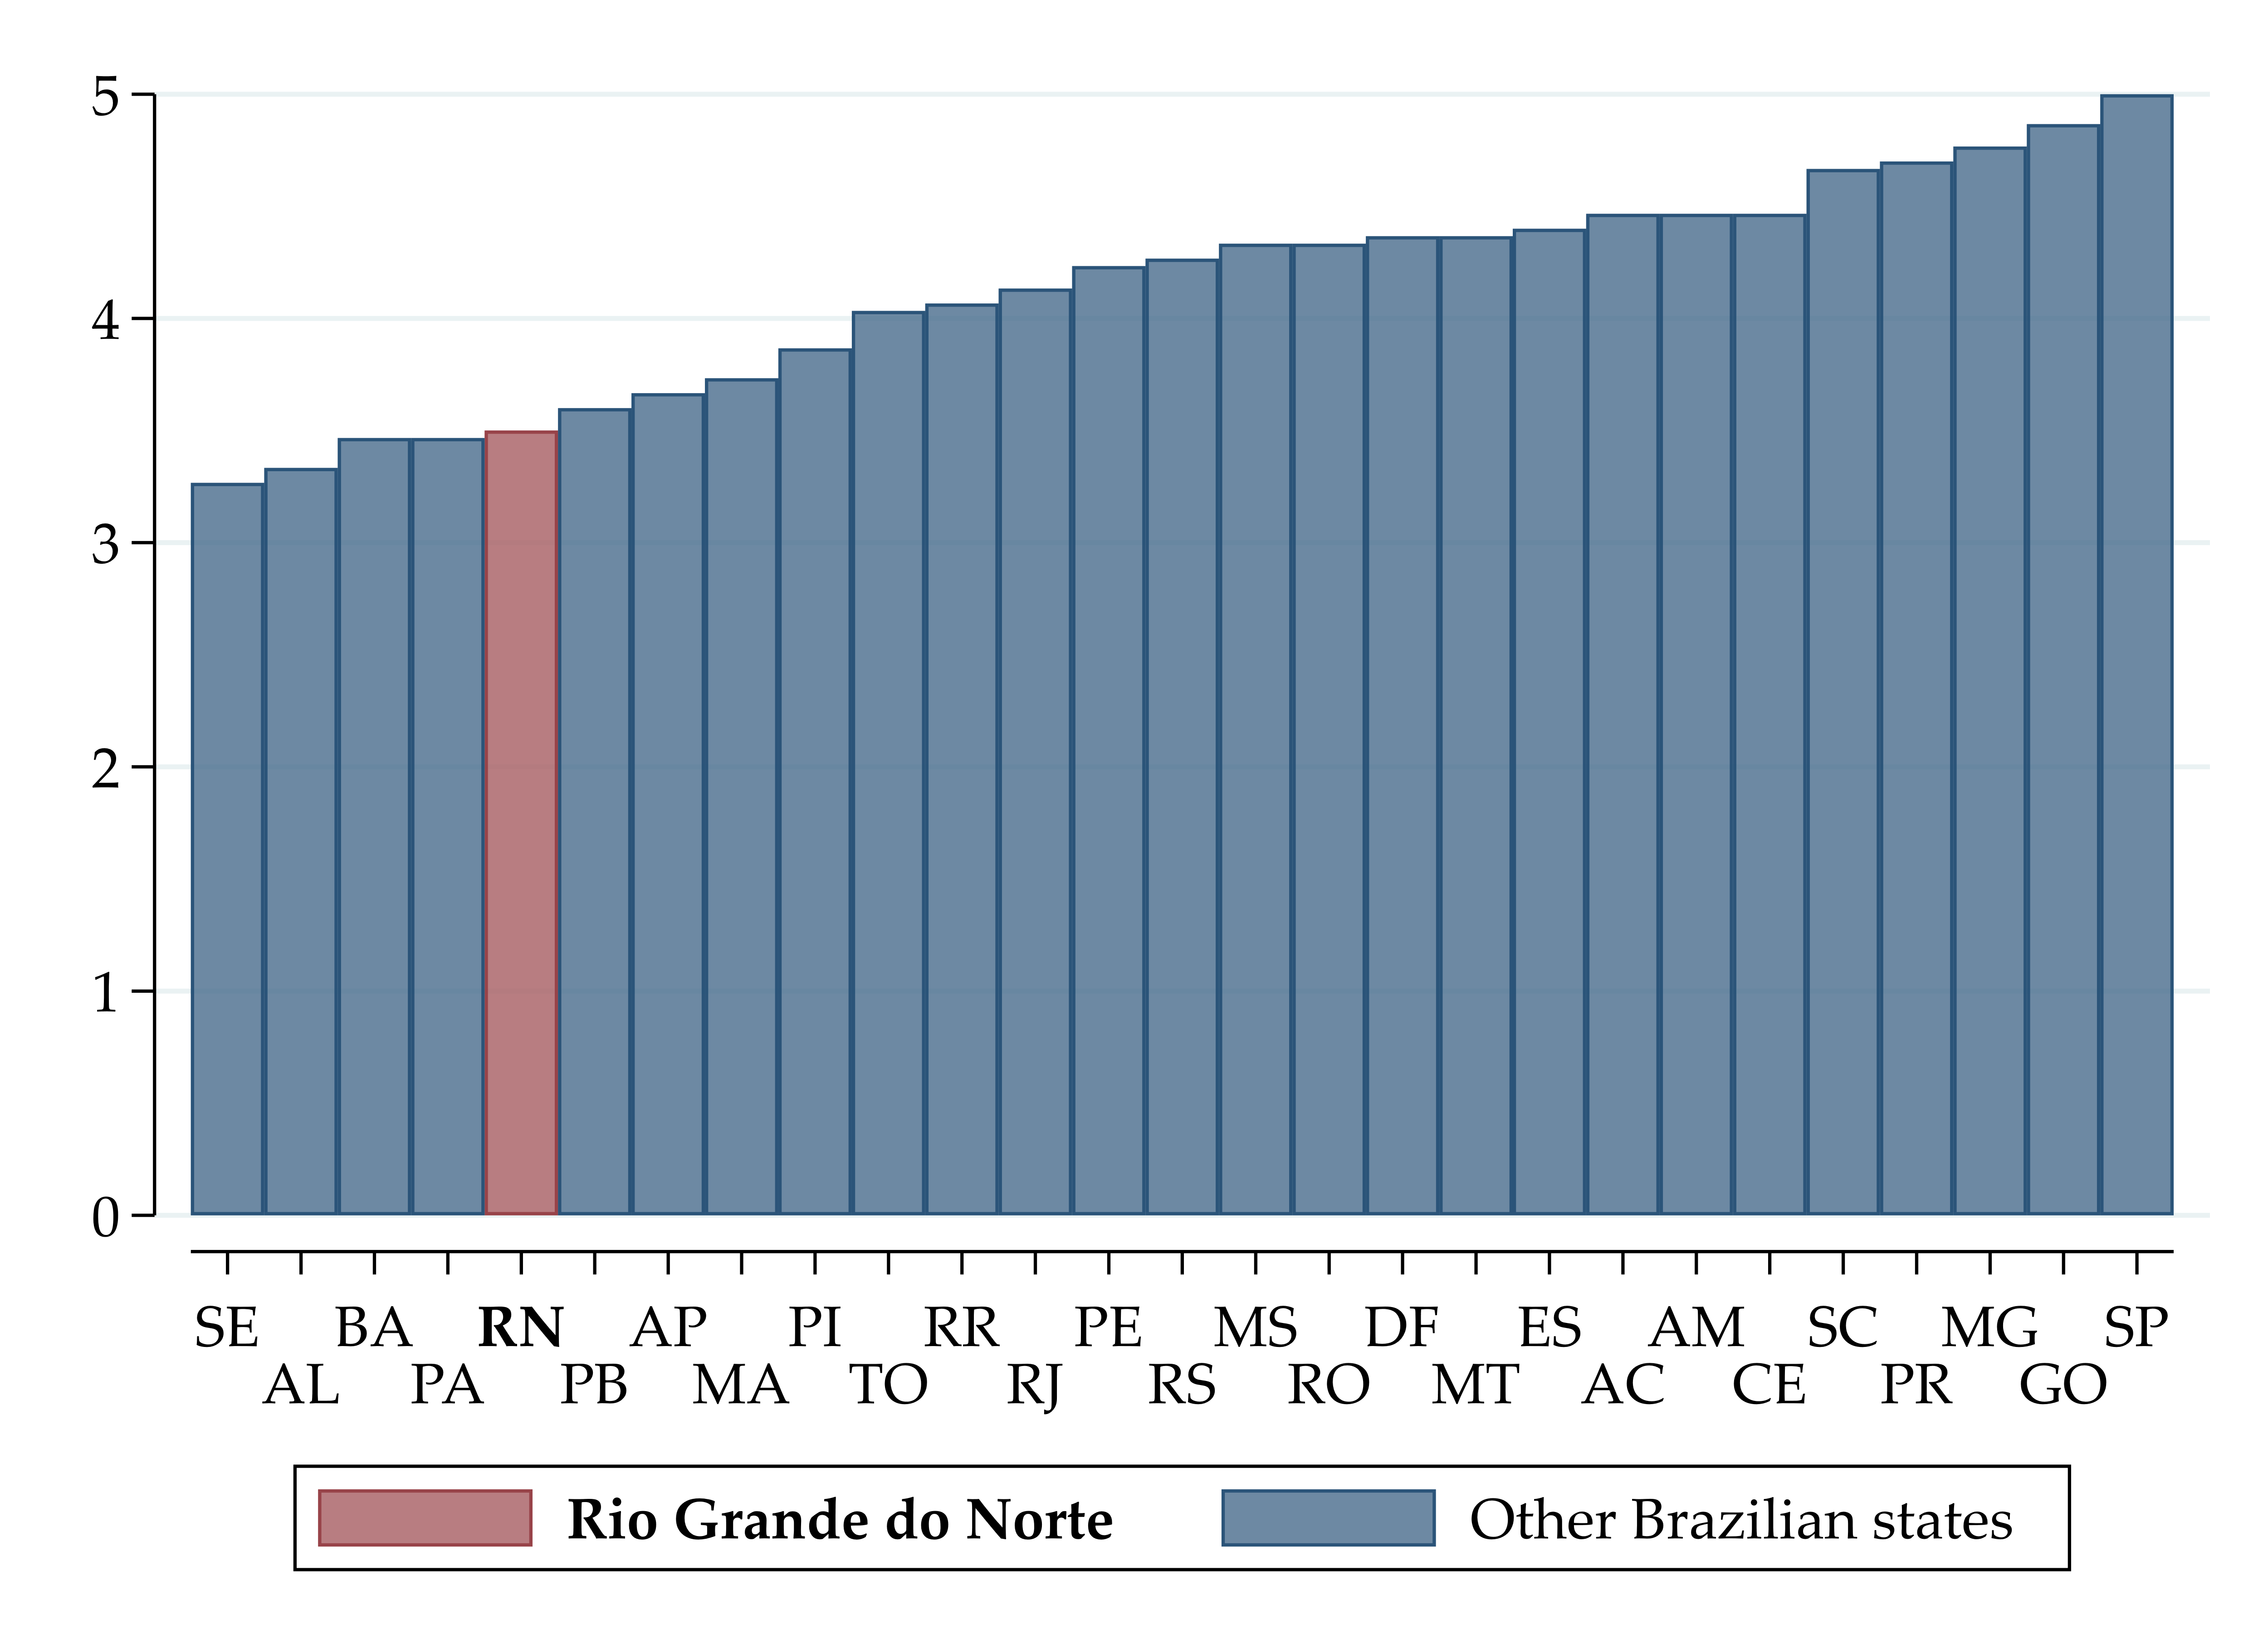
\includegraphics[width=13cm]{DataWork/Output/Figures/fig2-IDEB_byState.png}
		\begin{minipage}{0.835\textwidth}
			\small{\textit{Notes:} We use data from \textit{Instituto Nacional de Estudos e Pesquisas Educacionais Anísio Teixeira} (INEP) for state public schools. The IDEB index is defined at each education stage, i.e., for primary, middle, and secondary schools. The bars show the average IDEB across these three IDEB indices, by state in 2015.}
		\end{minipage}
	\end{figure}
	\FloatBarrier 
	
	%%%%%%%%%%%%%%%%%%%%%%% PIP %%%%%%%%%%%%%%%%%%%%%%%%%%%%%%%%
	
	\subsection{\textbf{The Pedagogical Innovation Project (PIP)}} \label{sec:pip}
	
	The Pedagogical Innovation Project (\textit{Projeto de Inovação Pedagógica} -- PIP) was developed by the RN Secretariat of Education (SEE) and aimed at improving both student progression and learning outcomes in primary and secondary schools. The program targets Grades 4, 5, 6 and 10, the grades with the most critical dropout and retention rates. The intervention has three main elements: 1) High degree of autonomy for schools to design and implement a project based on a context-specific diagnostic of the main challenges, with the SEE having only a advisory role to assure minimum quality standards; 2) Continuous technical support to schools for the design and implementation of the project ; 3) A grant to implement the project. 
	
	The decentralized approach of PIP sought to ensure the relevance of the interventions as well as motivate teachers and students. The design of the project is based on the premise that: i) school staff are better equipped than central-level bureaucrats to identify solutions to the school-specific problems; ii) allowing school staff autonomy over the selection and development of interventions motivates teachers by giving them the opportunity to implement activities of their authorship; iii) innovative projects can engage students and improve student-teacher interactions. The PIP was launched in 2014 and between the 2015 to 2018 school years covered a total of 397 of the 639 state schools.
	
	\subsubsection*{Project Development} \label{sec:project}
	
	Schools are invited to participate in a three-day workshop on innovative and project-oriented teaching practices. Each invited school should bring a Pedagogical Coordinator and the School Principal, who are responsible for the implementation of the project in the school. The workshop explores the concept of pedagogical innovation through seminars and round-table discussions. During break-out sessions participants identify the main pedagogical challenges they face and discuss how the innovation concepts would fit to their context. Each school is provided an individualized report card comparing their test scores and passing grades with average of the State, region, and their city.
	
	Following the workshop, each school is assigned a mentor (\textit{professor orientador}), who is part of the SEE central team.\footnote{Mentors are selected based on their experience with implementing pedagogical projects in schools and all are existing staff of the state secretariat.} Each mentor is assigned to 10 schools on average. The mentor first works with the school to prepare a diagnostic of their most critical challenges, such as low academic performance, grade retention, indiscipline, lack of motivation, or school dropout. Based on the diagnostic, schools identify possible drivers and propose an innovative and actionable plan to improve the targeted education outcomes. The mentors support schools to develop a broad project, including interdisciplinary elements, concepts of learning spaces outside the classroom, and highlight the importance of pedagogical planning and management. Many of the innovative practices are linked to use of information and communication technologies, such as the use of computer and science lab and the development of school radio and school-related video productions. Schools are also encouraged to include other pedagogical activities outside the school such as visits to local communities and cultural groups. The mentor then works with the school to translate the diagnostic and proposed project into a detailed action plan that is reviewed by the State Secretary of Education of Rio Grande do Norte. In this process, schools are encouraged to explore settings beyond traditional lecture style lessons to improve student-teacher interactions and to embed their project across disciplines, increasing coordination across subjects. 
	
	\subsubsection*{Implementation Support and Monitoring} \label{sec:implement}
	
	Schools with approved proposals are awarded with a fixed amount of funding to execute their projects. Schools can only spend the funds on inputs directly related to their project. The grant amount depends on the number of classes included in the project and ranges from R\$ 30,000 to 45,000 (US\$ 7,576 to 11,364).\footnote{Using exchange rate on 12/31/2015.} Figure \ref{fig:grant} shows the allocation rule and the percentage of schools by grant amount awarded. The average transfer per enrolled student was R\$ 838.40, the equivalent of about \$ 210. To receive the financial support, schools are required to obtain a clearance certificate, which indicates they are in compliance with Federal, State and Municipal fiscal bodies, following normal regulation to receive transfers. This turned out to be a large bottleneck and many schools implemented the interventions without receiving funding initially. The implications will be further explored in Section \ref{sec:mechanism}.
	
	\vspace{6pt}
	
	% Grant
	\begin{figure}[ht!]
		\caption{Allocation of Resources by Type of Grant}
		\label{fig:grant}
		\centering
		
		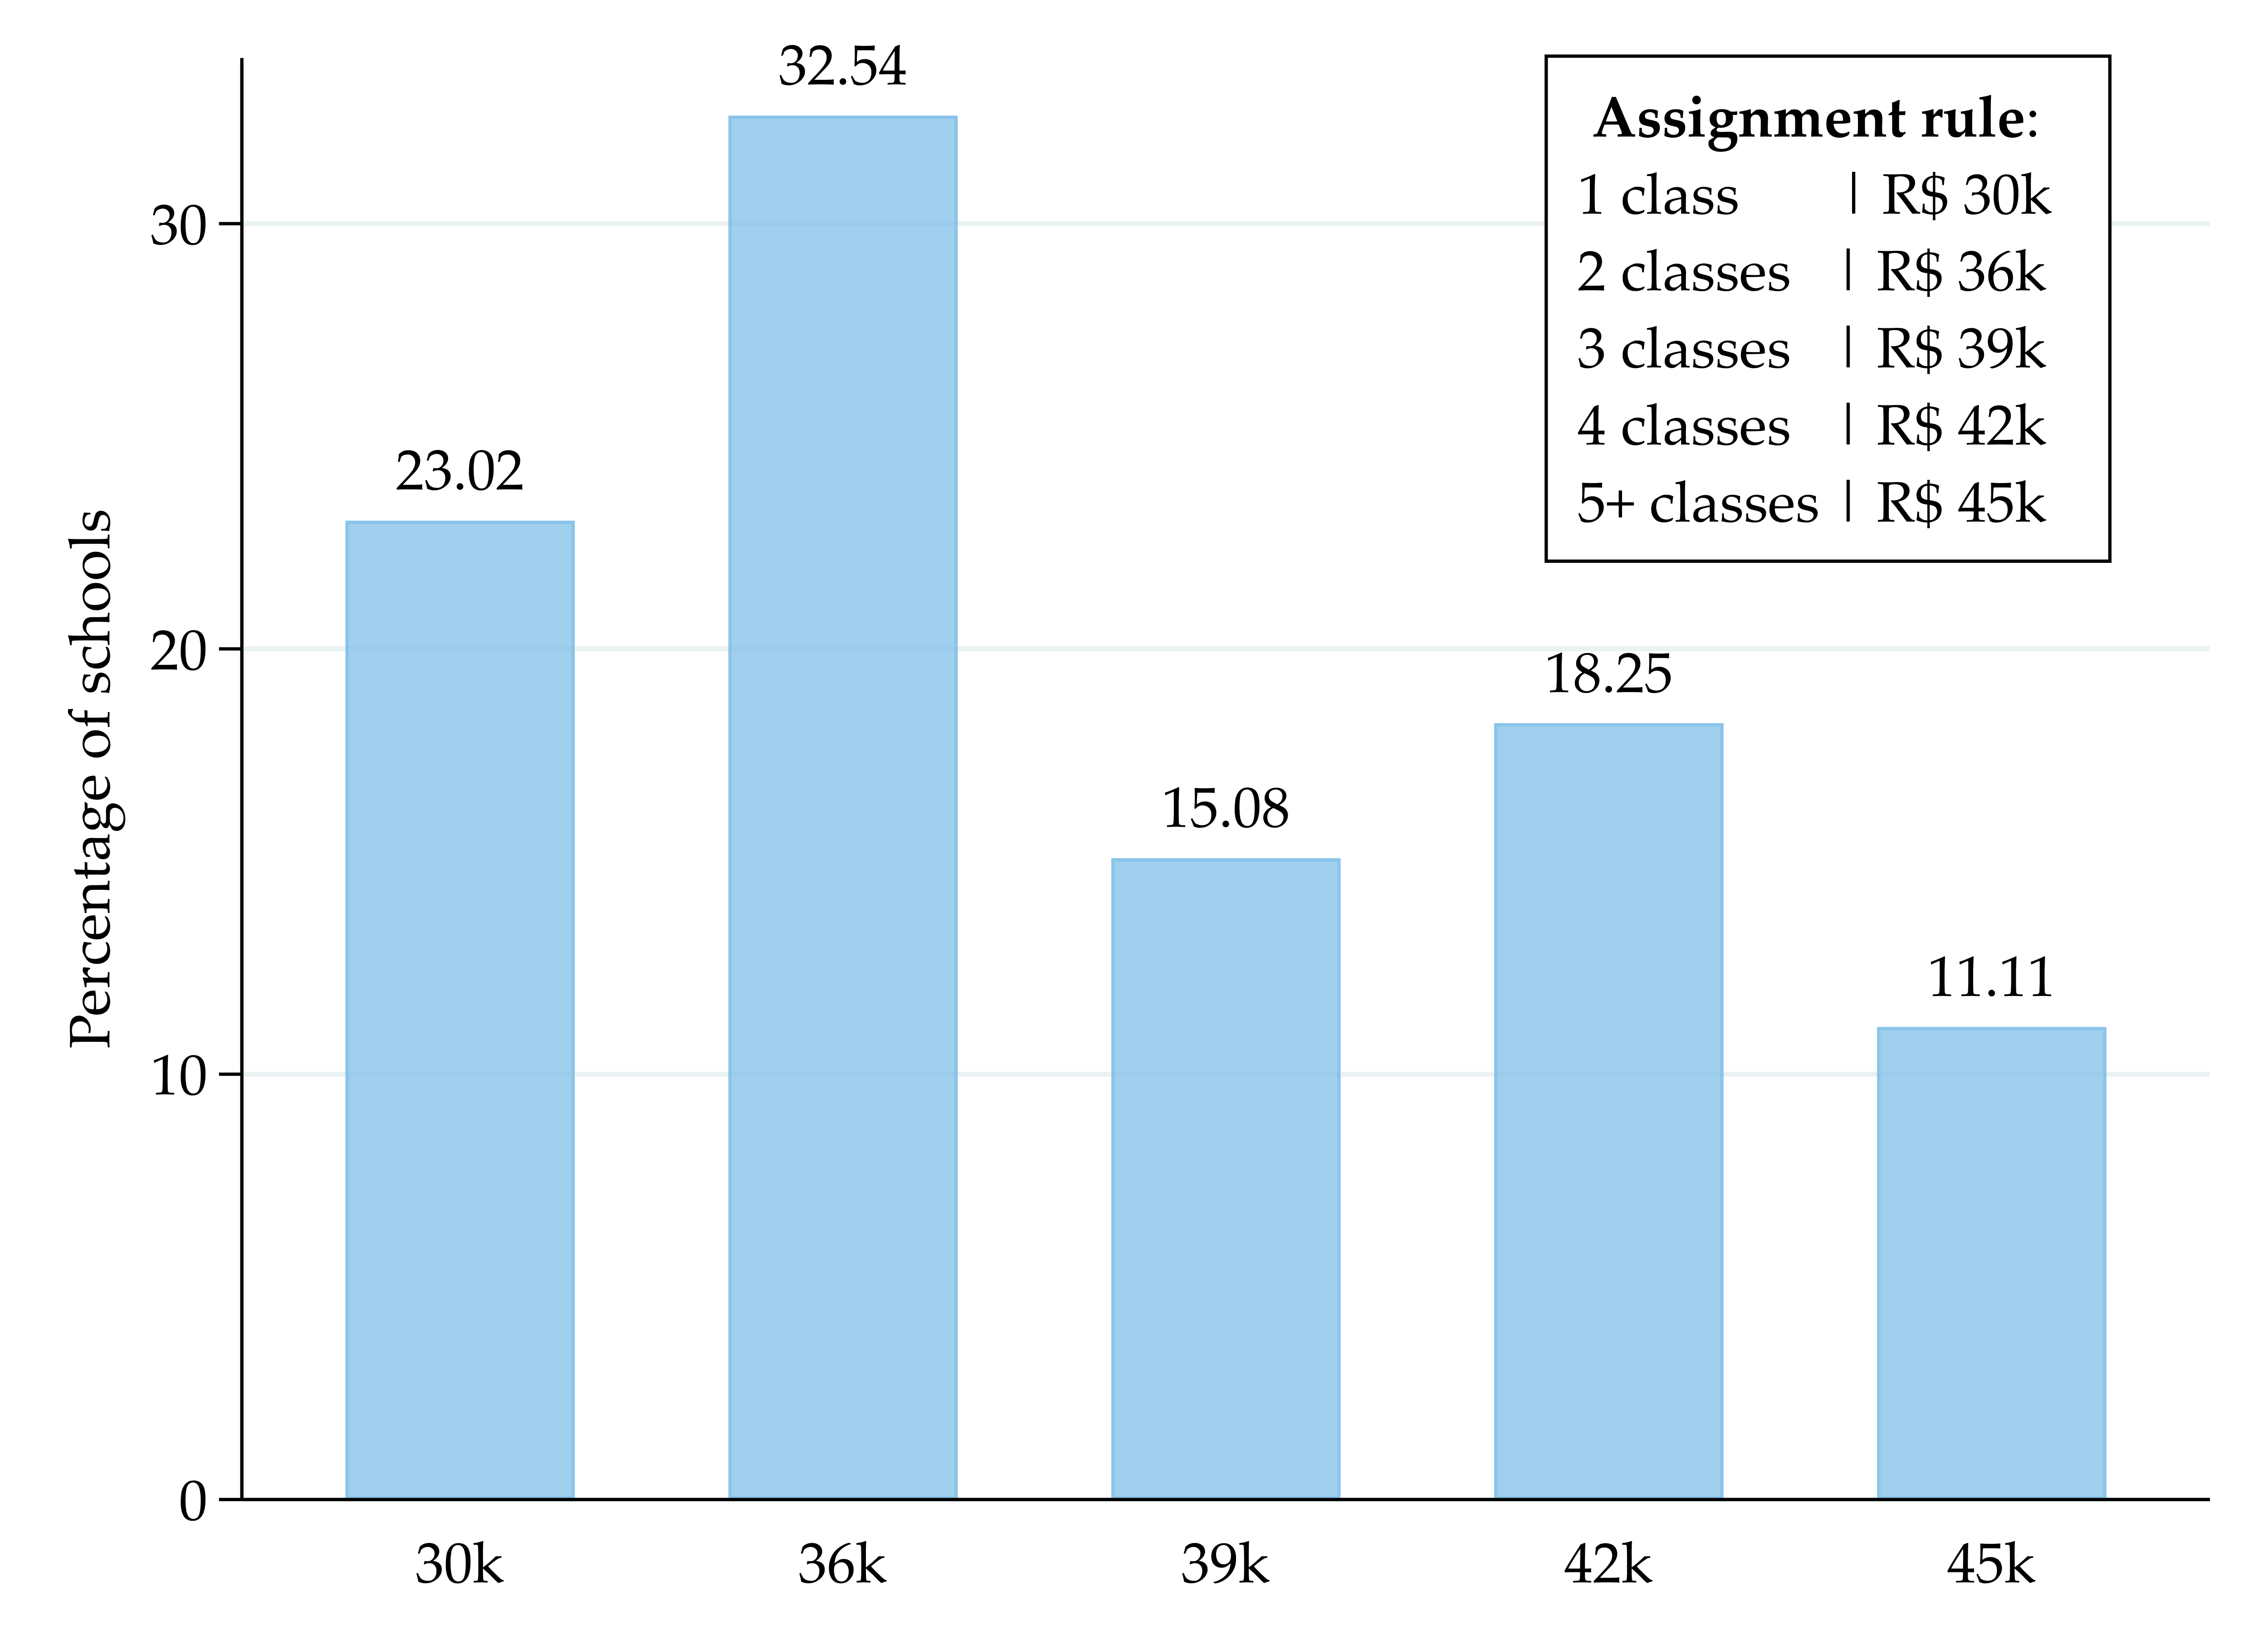
\includegraphics[width=13cm]{DataWork/Output/Figures/fig3-grant.png}
		
		\begin{minipage}{0.8\textwidth}
			\small{\textit{Notes:} The bars show the percentage of schools by the type of grant they were assigned to receive through PIP (ranging from 30,000 to 45,000). The values are in Brazilian Reais, which were worth 0.25 US at the beginning of 2016.}
		\end{minipage}
		
	\end{figure}
	%
	
	Through subsequent visits and remote follow up, mentors closely support the implementation of the projects. Mentors help schools obtain the necessary paperwork to access the funding and prepare procurement of materials and review the timeline and overall goals. Besides supporting the project implementation, the mentors encourage teachers to implement the project across different subjects and integrate the pedagogical contents and practices into the regular curriculum. The project is coordinated by two teachers, but implemented across all subjects in a grade as much as possible. 
	
	
	%%%%%%%%%%%%%%%%%%%%%%% DESIGN AND DATA %%%%%%%%%%%%%%%%%%%%%%%%%%%%%%%%
	
	\section{Experimental Design and Data} \label{sec:design_data}
	
	The PIP was launched in 2014 with implementation taking place in the 2015 school year. Each year a subset of schools joined the project. Our study focuses on the cohort of 2016. This section further details the selection of participating schools and data sources.
	
	\subsection{Experimental Design} \label{sec:experiment}
	
	To ensure enough operational capacity, only a sub-sample of schools were selected to participate each year. The RN SEE aimed to support a total of 130 schools in the 2016 school year. To determine the pool of eligible schools for that year, three filters were applied. First, only schools that would not change director between the 2015 and 2016 school year were included to ensure buy-in for the prepared projects. State legislation requires directors to change schools every 2 years, resulting in about half the schools changing director every year.\footnote{As a result none of schools from the first 2015 cohort were considered.}\textsuperscript{,}\footnote{This legislation has since slightly changed to allow for directors to stay on longer.} Second, the 2016 edition targeted the final grade of primary education (5\textsuperscript{th} grade), the first grade of lower secondary education (6\textsuperscript{th} grade) and the first grade of upper secondary education (10\textsuperscript{th} grade).\footnote{Other editions of the program included 4\textsuperscript{th} grade.} Only schools offering at least one of those three grades were considered. Finally, schools that participate in the Federal project ProEMI (\textit{Ensino Médio Inovador)} are not eligible.\footnote{\textit{Ensino Médio Inovador} (Innovative High School project -- ProEMI) was established in 2009 by the Ministry of Education as a policy aimed to support innovative curricular projects in upper secondary schools through technical and financial assistance.} Out of 639 state schools, 299 were eligible to receive the PIP project in 2016. The final selection of participating schools was done randomly, which forms the basis of our identification strategy. 
	
	The randomization was stratified by school grade and region. From the 2015 PIP cohort we learned that schools typically participate in just one grade. The SEE preferred to focus on higher grades, which is typically where schools experience more challenges. Therefore, schools offering several of the target grades (5\textsuperscript{th}, 6\textsuperscript{th} and 10\textsuperscript{th}) are assigned to participate for the highest target grade they offer. The state is divided in 4 regions and with t3he  grade levels this resulted in a total of 12 strata. In each stratum, around 40\% of the schools were allocated to the treatment group. In each selected school only the highest target grade, i.e., 5\textsuperscript{th}, 6\textsuperscript{th}, or 10\textsuperscript{th}, is selected to participate. Larger schools may have more than one class in a grade, in which case all classes, and thus students, in the selected grade participate. Not all teachers of a grade necessarily participate. Selection of teachers is decided within schools and is likely not random. When analyzing student and teacher outcomes we always consider all students and all teachers of the selected grade. 
	
	The randomization resulted in 130 eligible schools in the treatment group and 169 in the control group (Panel A in Table \ref{tab:sample}). All selected schools were invited to the workshops held in the final months of the 2015 school year. The randomization was performed based on the 2015 school census. After the start of the 2016 school year a few schools had closed or no longer offered the grade that had been selected for the intervention.\footnote{Eight schools had closed, six were not offering regular classes anymore, four were selected for the 5\textsuperscript{th}-grade experimental group but were not offering 5\textsuperscript{th} grade anymore, and one was in the 6\textsuperscript{th} grade group but was not offering 6\textsuperscript{th} grade anymore.} This leaves us with a final sample of 280 schools effectively allocated to the experiment at the beginning of the 2016 school year (Panel B in Table \ref{tab:sample}), 126 in the treatment group and 154 in the control group. The geographical distribution and treatment assignment of these schools is shown in Figure \ref{fig:treat_map}. Across the selected grades in each school, a total of 19,899 students were included in the experiment, 9,432 in treated schools and 10,467 in control schools (Panel C in Table \ref{tab:sample}).  
	
	\vspace{15pt}
	
	% Sample sizes for the experiment
	\begin{table}[ht!]
		\caption{Sample}
		\label{tab:sample}
		\centering
		\begin{adjustbox}{max width=\textwidth}
\begin{tabular}{lccc} \hline \hline
\multicolumn{4}{c}{\textbf{A) Number of eligible schools}}      \\ \hline
                       & Treatment     &   Control     & Total \\ 
\cmidrule(lr){2-4}
5th  grade &47&60&107 \\ 
6th  grade &48&63&111 \\ 
10th grade &35&46&81 \\ 
\cmidrule(lr){2-4}
Total      &130&169&299 \\ 
\hline \\ \hline
\multicolumn{4}{c}{\textbf{B) Effective number of schools}} \\ \hline
                       & Treatment     &   Control             & Total \\ 
\cmidrule(lr){2-4}
5th  grade &45&52&97 \\ 
6th  grade &46&59&105 \\ 
10th grade &35&43&78 \\ 
\cmidrule(lr){2-4}
Total     &126&154&280 \\ 
\hline \\ \hline
\multicolumn{4}{c}{\textbf{C) Number of enrolled students}} \\ \hline
                       &  Treatment    &   Control     & Total              \\ 
\cmidrule(lr){2-4}
5th  grade &4061&3952&8013 \\ 
6th  grade &2517&2871&5388 \\ 
10th grade &2854&3644&6498 \\ 
\cmidrule(lr){2-4}
Total      &9432&10467&19899 \\ 
\hline \hline \end{tabular}
\end{adjustbox}

	\end{table}
	%
	
	% Map
	\begin{figure}[ht!]
		\caption{Geographical Distribution of Schools by Treatment Status}
		\label{fig:treat_map}
		\centering
		
		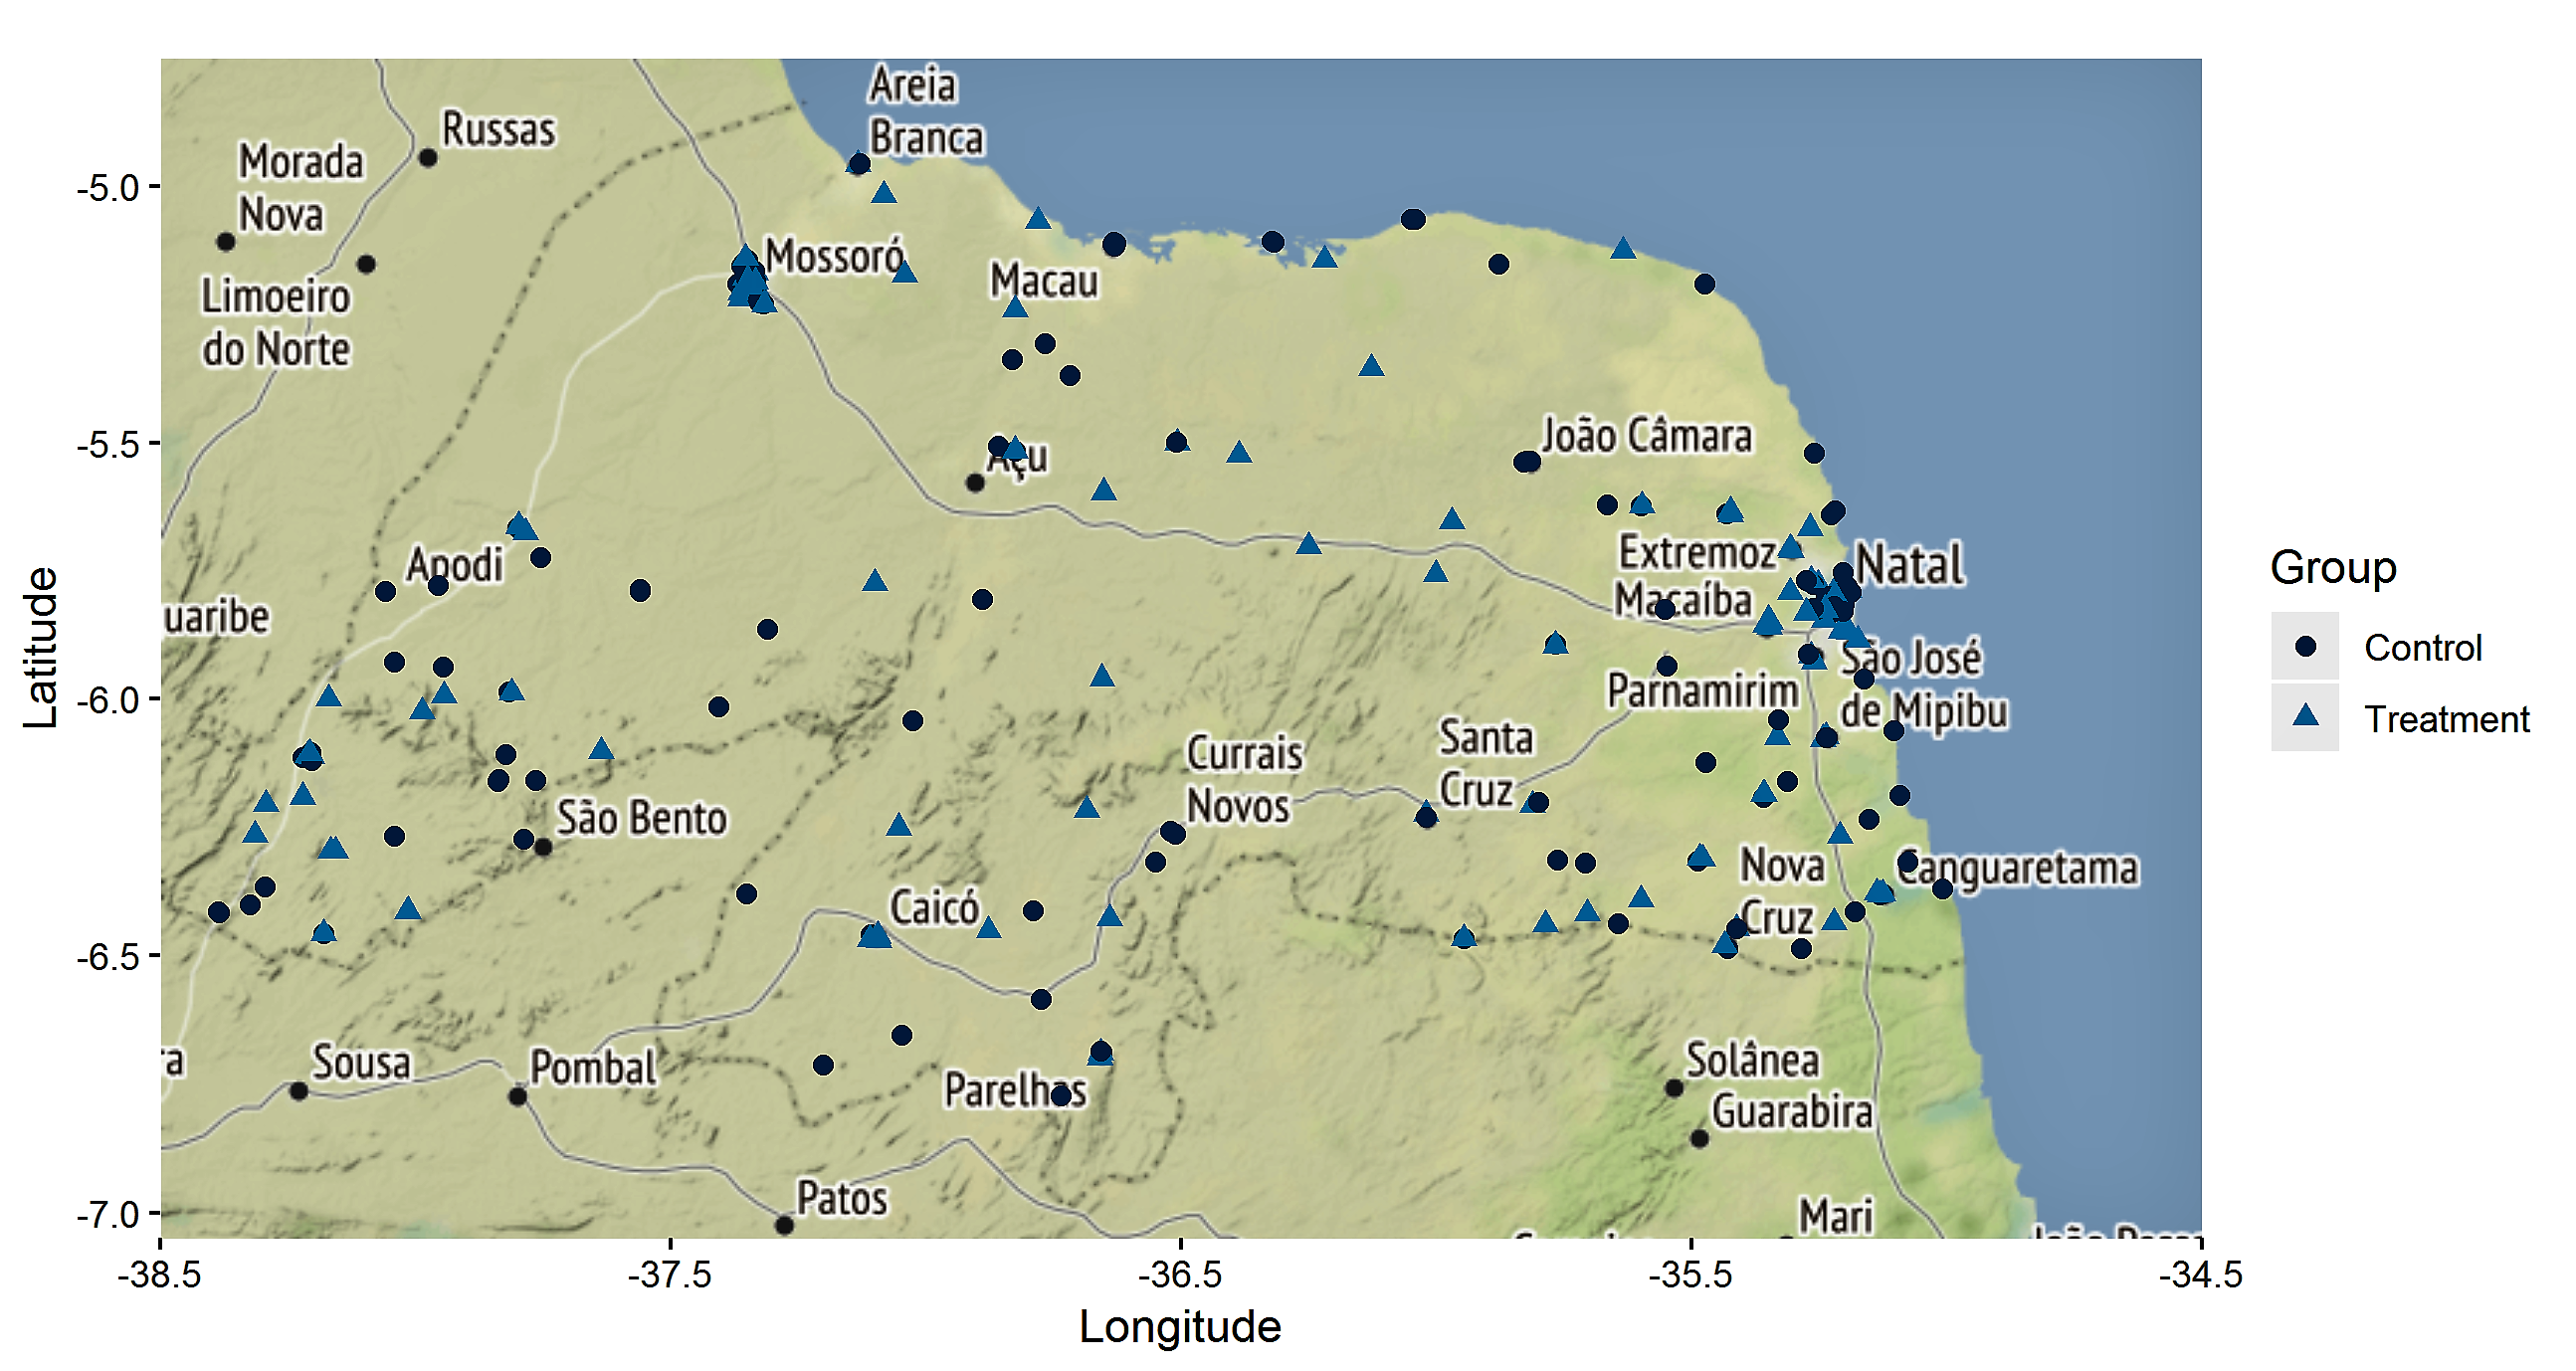
\includegraphics[width=15cm]{DataWork/Output/Figures/fig4-treat_map.png}
		
		\begin{minipage}{0.92\textwidth}
			\small{\textit{Notes:} GPS locations were extracted by scraping Google Maps API with school names. All but 6 schools in the experimental sample, 3 in the control and 3 in the treatment group, were not properly located using this method.}
		\end{minipage}
	\end{figure}
	%
	
	\clearpage
	
	\subsection{Data} \label{sec:data}
	
	To assess the impact of the PIP we leverage three main sources of data. We use administrative data, such as the Brazilian school census and data from the SEE, and collect data on cognitive and socio-emotional skills.
	
	\subsubsection*{Administrative Data} 
	We use administrative data from both the annual national school census and the state's education monitoring system to obtain school, teacher and student characteristics and progression.\footnote{The school census is carried out on an annual basis by the \textit{Instituto Nacional de Estudos e Pesquisas Educacionais Anísio Teixeira} (INEP) of the Brazilian Ministry of Education (MEC).} It contains data on overall school characteristics, such as location, presence of a library, science lab and internet, number of teachers, students and classes.\footnote{We extract school location and distance from the capital of the state, Natal, by scraping Google Maps API with school names.} The census also allows us to track individual teachers and students over time, even if they move to other schools within the state.\footnote{Brazilian Education Census is implemented in two stages. At the beginning of the school year (i.e., May-July) initial student enrollment data is collected and the survey of school, teacher and students' characteristics. In February-March of the following year, data is collected on passing/retention and on ``movement'', which includes dropout and transfers.} The state's monitoring system, the \textit{Sistema Integrado de Gestão da Educação} (SIGEduc) portal, provides data on passing, dropout, and retention rates at the grade level.\footnote{Progression rates are reported at the end of the school year (i.e., February-March) by principals, and then validated by INEP.} Where possible the analysis of the results uses both sources. Finally, the SEE provided data on school directors and on the implementation of the PIP, such as the score of the proposal, resources allocated to schools and execution of the project. Rate of implementation of the proposed plan is assessed by the mentor at each visit.  
	
	\subsubsection*{Learning Outcomes}
	To measure student learning, we use the standardized state exam in math, Portuguese, social and human sciences, which were administered to 5\textsuperscript{th}, 6\textsuperscript{th}, 10\textsuperscript{th} and 12\textsuperscript{th} grades at the end of the 2016 school year. The RN standardized exam was introduced in 2016 and expanded to include all the PIP priority grades. For math and Portuguese, we obtain the scores re-scaled to the national standardized test (SAEB), which allows us to put the impact on student learning in the Brazilian wide context. 
	
	\subsubsection*{Socio-Emotional Skills} 
	To analyze the impact on socio-emotional skills, we collect a measure of the Big Five personality traits (neuroticism, extroversion, conscientiousness, agreeableness, openness).\footnote{The taxonomy of the five-factor model of personality we follow in this paper has been developed in the psychology literature following seminal work by \citet{fiske1949consistency}.} We use a self-reported test developed and adapted to younger students in Brazil by the \textit{Instituto Ayrton Senna} (IAS). This test, and equivalent, are widely used in the literature to assess socio-emotional skills.\footnote{See \cite{kautz2014fostering} for a review of the recent advances on measuring socio-emotional skills.}\textsuperscript{,}\footnote{Research has shown that individuals with the same level of a trait may assess themselves at very different levels on a Likert scale \citep{primi2016anchor}. To address this issue, we administered a set of anchoring-vignettes which help reveal the respondent latent scale and response style allowing us to calibrate the individual responses following the method suggested in \cite{primi2016anchor}.The vignettes describe three hypothetical individuals that represent three clearly distinct points on a scale (low, medium and high). Students are asked to assess the personality trait of each of the characters along a 1-5 Likert scale. The student self-evaluation is then calibrated to a 1-7 scale according to her response to the vignette.} The test was administered at the end of the 2016 school year to the grade that entered the randomization (highest grade offered among 5\textsuperscript{th}, 6\textsuperscript{th} and 10\textsuperscript{th} grade, see Section \ref{sec:experiment}). In case a school had multiple classes in the same grade, one class was randomly chosen.  
	
	
	\subsection{Validity of the Experiment} \label{sec:balance}
	
	\subsubsection*{Randomization}
	To examine whether the randomization resulted in balanced samples across control and treatment groups, we compare observable characteristics prior to roll-out of the project. Table \ref{tab:baltab} shows several characteristics at the school, grade, teacher and student level, including some of the key outcomes of the intervention, such as repetition and dropout rates. For grade, teacher and student comparisons, we only consider the classes in the eligible grade for that school (see description in Section \ref{sec:experiment}). Columns 2 and 4 show the means in the treatment and control groups. In column 5, we report both standard p-values based on t-test of differences in the means and p-values computed using randomization inference.\footnote{See \cite{young2019channelling} on the importance of randomization statistical inference in experimental setups and \cite{hess2017randomization} for a guideline on its implementation.} Generally we find no statistical differences when comparing the treatment and control groups. A joint significance test of school and student characteristics confirm that these variables do not jointly predict treatment assignment (F-stat of 0.69 and 1.76, respectively).
	
	Randomization was done by grade level, to test the validity of the sub-group analysis, we also report p-values for the comparison in each grade in columns 6-8. We find a statistically significant, yet small, difference in age of 6\textsuperscript{th} graders. The control group is on average 0.25 years older than the treatment group. In the analysis we check robustness of the results to the inclusion of this unbalanced variable as control.
	
	% Balance table comparing treatment and control schools
	\vfill
	\begin{table}[ht!]
		\caption{Balance Table}
		\label{tab:baltab}
		\centering
		\begin{adjustbox}{max width=\textwidth}
			\begin{tabular}{lcccccccc} \hline \hline
				                  & \multicolumn{5}{c}{\textbf{All schools}}                                      & 5th Grade    & 6th Grade    & 10th Grade   \\                       
                        \cmidrule(lr){2-6} \cmidrule(lr){7-7} \cmidrule(lr){8-8} \cmidrule(lr){9-9}                                                                    \\[-2ex]               
                  & (1)                  & (2)         & (3)                   & (4)           & (5)          & (6)              & (7)          & (8)                  \\                               
                  &                      &             &                               &                       & T-test       & T-test           & T-test       & T-test               \\                               
                  &                      & Control &                           & Treatment & P-value      & P-value      & P-value      & P-value              \\                               
 Variable & N/[Clusters] & Mean/SE &  N/[Clusters] & Mean/SE   & [RI p-value] & [RI p-value] & [RI p-value] & [RI p-value] \\ \hline \\[-2ex]
\multicolumn{9}{c}{\textbf{Panel A -- School characteristics}}                                                                                                                         \\[0.5ex] \hline 
                                   \addlinespace[0.75ex] Has access to internet & 154 & 0.922 & 124 & 0.960 & 0.197 & 0.228 & 0.413 & 0.835 \\    &  & (0.022) &  & (0.018) & [0.223] & [0.371] & [0.468] & [1.000] \\  Has library & 154 & 0.669 & 124 & 0.661 & 0.957 & 0.970 & 0.301 & 0.046 \\   &  & (0.038) &  & (0.043) & [0.964] & [1.000] & [0.333] & [0.074] \\  Has sciences lab & 154 & 0.143 & 124 & 0.169 & 0.412 & N/A & 0.721 & 0.311 \\   &  & (0.028) &  & (0.034) & [0.426] & [1.000] & [1.000] & [0.349] \\  Located in urban area & 154 & 1.169 & 126 & 1.127 & 0.339 & 0.197 & 0.835 & 0.389 \\   &  & (0.030) &  & (0.030) & [0.392] & [0.277] & [1.000] & [0.538] \\  Distance to Natal (km) & 151 & 152.086 & 123 & 142.837 & 0.877 & 0.760 & 0.915 & 0.599 \\   &  & (9.140) &  & (10.375) & [0.876] & [0.756] & [0.915] & [0.585] \\  Number of employees & 154 & 29.422 & 124 & 29.589 & 0.889 & 0.824 & 0.718 & 0.510 \\   &  & (1.136) &  & (1.222) & [0.887] & [0.826] & [0.713] & [0.511] \\  Number of students & 154 & 361.903 & 124 & 374.621 & 0.697 & 0.636 & 0.904 & 0.854 \\   &  & (19.116) &  & (24.671) & [0.697] & [0.643] & [0.900] & [0.849] \\  Number of classes & 154 & 14.669 & 124 & 14.573 & 0.870 & 0.777 & 0.634 & 0.774 \\   &  & (0.666) &  & (0.825) & [0.867] & [0.777] & [0.623] & [0.775] \\  Students per class & 154 & 24.216 & 124 & 24.802 & 0.388 & 0.263 & 0.171 & 0.310 \\   &  & (0.509) &  & (0.514) & [0.398] & [0.260] & [0.170] & [0.316] \\ \hline \\[-2ex]                                                                                                                                                                                                                             
\multicolumn{9}{c}{\textbf{Panel B -- Grades assigned to the intervention}}                                                                                            \\[0.5ex] \hline 
                       \addlinespace[0.75ex] Passing rate & 154 & 70.714 & 123 & 72.637 & 0.389 & 0.372 & 0.194 & 0.412 \\    &  & (1.434) &  & (1.545) & [0.378] & [0.374] & [0.190] & [0.398] \\  Drop-out rate & 154 & 8.023 & 123 & 8.183 & 0.811 & 0.381 & 0.243 & 0.123 \\   &  & (0.780) &  & (0.943) & [0.810] & [0.366] & [0.255] & [0.126] \\  Retention rate & 154 & 21.263 & 123 & 19.180 & 0.265 & 0.475 & 0.372 & 0.761 \\   &  & (1.201) &  & (1.298) & [0.260] & [0.483] & [0.359] & [0.754] \\  Teacher turnover rate & 149 & 0.350 & 123 & 0.312 & 0.286 & 0.578 & 0.684 & 0.239 \\  &  & (0.025) &  & (0.023) & [0.295] & [0.584] & [0.691] & [0.252] \\ \hline \\[-2ex]                                                                                                                                                                                              
\multicolumn{9}{c}{\textbf{Panel C -- Teacher characteristics}}                                                                                                                        \\[0.5ex] \hline 
                           \addlinespace[0.75ex] Age & 1021 & 40.296 & 861 & 40.087 & 0.666 & 0.213 & 0.744 & 0.704 \\    & [153] & (0.331) & [124] & (0.363) & [0.628] & [0.240] & [0.738] & [0.645] \\  Gender (male $= 1$) & 1021 & 0.471 & 861 & 0.511 & 0.229 & 0.884 & 0.123 & 0.687 \\   & [153] & (0.016) & [124] & (0.019) & [0.297] & [1.000] & [0.189] & [0.735] \\  White & 715 & 0.491 & 582 & 0.529 & 0.256 & 0.937 & 0.719 & 0.230 \\   & [146] & (0.023) & [110] & (0.023) & [0.197] & [0.933] & [0.701] & [0.154] \\  Has completed tertiary education & 1021 & 0.937 & 861 & 0.940 & 0.840 & 0.114 & 0.908 & 0.229 \\   & [153] & (0.010) & [124] & (0.010) & [0.843] & [0.105] & [1.000] & [0.143] \\  Has specialization and/or master & 1021 & 0.405 & 861 & 0.389 & 0.724 & 0.750 & 0.147 & 0.092 \\   & [153] & (0.019) & [124] & (0.019) & [0.698] & [0.754] & [0.103] & [0.051] \\ \hline \\[-2ex]                                                                                                                                                                                                                             
\multicolumn{9}{c}{\textbf{Panel D -- Student characteristics}}                                                                                                                        \\[0.5ex] \hline 
                         \addlinespace[0.75ex] Age & 9558 & 12.725 & 8827 & 12.401 & 0.088 & 0.275 & 0.059 & 0.987 \\    & [146] & (0.266) & [120] & (0.276) & [0.092] & [0.289] & [0.080] & [0.989] \\  Gender (male $= 1$) & 9560 & 0.517 & 8828 & 0.516 & 0.579 & 0.789 & 0.189 & 0.333 \\   & [146] & (0.007) & [120] & (0.008) & [0.585] & [0.789] & [0.214] & [0.343] \\  White & 6245 & 0.354 & 5819 & 0.335 & 0.244 & 0.341 & 0.660 & 0.566 \\   & [142] & (0.020) & [118] & (0.024) & [0.271] & [0.367] & [0.693] & [0.628] \\  Receives \textit{Bolsa Família} & 9560 & 0.319 & 8828 & 0.313 & 0.947 & 0.496 & 0.262 & 0.860 \\   & [146] & (0.025) & [120] & (0.024) & [0.948] & [0.504] & [0.286] & [0.876] \\      
\hline \hline \\[-2ex]

				\multicolumn{9}{@{}p{1.55\textwidth}}{\textit{Notes}: For school and grade level comparisons we use data from the 2015 Rio Grande do Norte school census (\textit{Instituto Nacional de Estudos e Pesquisas Educacionais Anísio Teixeira} -- INEP) and progression rates from \textit{Sistema Integrado de Gestão da Educação} (SIGEduc) portal. At the teacher and student level, we compare socio-demographics at the beginning of the year of the intervention, i.e., 2016, from that year Rio Grande do Norte school census. Teacher data regard only those teachers who taught in the classes involved in the project, and not from other grades. Student data regard students enrolled in those grades at the beginning of the school year. Two schools out of the 280 schools in the sample are missing in the census. Standard errors (SE) are robust in Panel A and B, and clustered at the school level in Panel C and D. Strata (i.e., region and grade) fixed effects are included in all the estimated regressions. We show both standard p-values and p-values computed using randomization inference (RI) with 10,000 repetitions for the whole sample and for each grade.}
			\end{tabular}
		\end{adjustbox}
	\end{table}
	\FloatBarrier
	%
	
	\subsubsection*{Attrition and Implementation}
	All 130 initially selected schools were invited to participate in the workshop, which occurred in late 2015. Of the 128 participating schools, all prepared and submitted a proposal. All submitted proposals were approved, some after modifications. At the beginning of the 2016 school year, four of the 130 selected treatment schools had closed or did not offer the target grade anymore, resulting in a final sample of 126 schools, all with approved projects.  Following approval, all schools received the first visit of the mentor at the beginning of the school year. Throughout the year, schools were meant to receive quarterly visits. Of the 126 schools, 109 received at least three visits along the school year, and 39 received all four visits. To receive the allocated funding, the schools had to provide proof that they did not have outstanding balance with federal, state or municipal tax collection agencies.\footnote{Although public schools do not pay taxes, they do need to file that they are exempt.} The lack of this documentation delayed the transfer of funds for most schools. Transfers were supposed to take place at the beginning of the school year in February, but the first transfers were only made in July. By the end of the school year of 2016, 90 schools had received the funding.\footnote{8 schools received the funding in the following year.} Despite the challenges with the transfer of resources, mentors worked with the schools to continue implementation of the activities proposed in their work plan. By the end of the school year 79.37\% of schools implemented at least 70\% of the planned activities. The main results presented in Section \ref{sec:results} take into consideration the original assignment in the experiment (Panel B in Table \ref{tab:sample}) and should therefore be interpreted as intent-to-treat (ITT) effects.
	
	\subsubsection*{Missing Data}
	Not all schools and students participated in the socio-emotional and proficiency test. Table \ref{tab:baltab_participation} compares participation rates between the control and treatment group. Overall, 84\% of schools participated in the socio-emotional test and 94\% participated in the state standardized tests. Among the participating schools, on average, 55\% of enrolled students took the socio-emotional test, and 69\% participated in the proficiency tests. Treated schools are more likely to participate in the socio-emotional test (91.3\% versus 77.9\%), while participation is balanced for the proficiency tests. Conditional on the school participating, the percentage of test takers is balanced for both tests, across all grades, suggesting no differential within school selection by treatment assignment. 
	
	To explore how the unbalanced participation of schools in the socio-emotional test may affect our results, we replicate the balance table restricting the sample to schools with at least one test-taker (Tables \ref{tab:baltab_socio_schoollevel} and \ref{tab:baltab_proficiencia_media_schoollevel}). We find similar balance results as for the complete sample. Taking the 2015 IDEB as a measure of school quality at baseline, we compare schools that participated in the socio-emotional test with those who did not, across treatment and control groups (Figure \ref{fig:predict_participation}). As expected treatment and control schools generally have similar IDEB scores ($p=0.98$). However, participating schools generally have better scores than non-participating schools ($p=0.02$). Yet this pattern appears to be equal among treatment and control groups ($p=0.62$). These results suggest that our results are likely unbiased estimates of the impacts of tested schools, yet they may not extend to the non-tested schools. 
	
	
	%%%%%%%%%%%%%%%%%%%%%%% RESULTS %%%%%%%%%%%%%%%%%%%%%%%%%%%%%%%%
	
	\section{Empirical Strategy and Results} \label{sec:methodology_results}
	\subsection{Empirical Strategy} \label{sec:methodology}
	
	We estimate the effect of randomly assigning schools to the project on our outcomes of interest with the following reduced-form specification,
	\begin{equation} \label{eq:OLS}
	y_{is} = \alpha + \beta \cdot T_{s} + \Sigma_{strata} + \varepsilon_{is}
	\end{equation}
	where $y$ is the outcome of interest for student $i$ in school $s$, $T_s$ is the indicator variable of treatment assignment, $\Sigma$ is a vector of strata dummies, and $\varepsilon$ is the error term. Standard errors are clustered at the school level.\footnote{Some estimates are obtained at the school level. In these cases, we employ robust standard errors.} Since not all assigned schools received all components of the project, as discussed in Section \ref{sec:experiment}, the parameter $\beta$ measures the ITT effect. We provide estimates of project impact for all schools pooled as well as for each grade separately. To check robustness of the results, we estimate the model adding controls, and we use interaction-weighted, regression-weighted and blocked difference-in-means estimators.\footnote{\cite{gibbons2018broken} show that, in the presence of heterogeneous treatment effects, fixed effects estimates are generally not a consistent estimator of the average treatment effect. The blocked difference-in-means approach uses strata sizes, instead of fixed effects, to weight the treatment effects estimates within each strata.}
	
	To explore potential distributional effects of the project we estimate unconditional quantile treatment effects (UQTE) effects following \cite{firpo2009unconditional}. Unlike the average effect, quantile treatment effects assess whether the impact of the project differs at distinct points (quantiles) of the outcome distribution. The UQTE has a similar interpretation as the average effect and it is estimated by computing the horizontal difference between accumulated (or marginal) distributions of treated and control outcomes for a given quantile. For example, the effect on the median is given by $UQTE_{0.5} = Q_{0.5}(Y_{T}) - Q_{0.5}(Y_{C})$, where $Y_{T}$ is the value of the outcome variable (e.g., test score) at the distribution median of the treated group and $Y_{C}$ is the value of the outcome variable at the distribution median of the control group.
	
	
	\subsection{Results} \label{sec:results}
	We begin the analysis with the key outcomes targeted by the project: student learning and progression indicators such as grade passing, repetition and dropout. In Section \ref{sec:mechanism} we look at intermediate outcomes, such as teacher-turnover and socio-emotional skills to shed light on the potential mechanisms leading to impacts on final outcomes.
	
	\subsubsection*{Learning Outcomes} \label{sec:skills}
	
	Table \ref{tab:test_studentlevel} shows ITT estimates on overall test scores as well as separated by subject and grade. We find large positive impact on learning outcomes among schools assigned to treatment, but for 6\textsuperscript{th} graders only. The intervention improved overall test scores for 6\textsuperscript{th} graders by 0.146 SDs, or 6 points compared to a mean in the control group of 163. Significant improvements are observed across all subjects but are more pronounced for math and Portuguese. For robustness, we re-estimate the model controlling for a vector of covariates\footnote{They include student's age, gender and race dummies (white, indigenous, black, or \textit{pardo}), whether they receive \textit{Bolsa Familia}, and whether they use school transportation.} and using alternative estimation strategies, such as interaction-weighted and regression-weighted estimators, blocked difference-in-means, as well as collapsing data at the school level. The results are very similar and are available in the Online Appendix.\footnote{The Online Appendix can be accessed through this \href{https://github.com/worldbank/brazil-pip-education/pip_app.pdf}{link}.} The quantile regression estimates for 6\textsuperscript{th} graders are presented in Figure \ref{fig:qreg_media_grade6} (average test score), and suggest gains across the board, with a more pronounced difference at the higher end of the grade distribution.\footnote{Quantile results disaggregated by subject are available in the Online Appendix.}
	
	% Impact on cognitive
	\vfill
	\begin{table}[ht!]
		\caption{Impact on Student Learning}
		\label{tab:test_studentlevel}
		\centering
		\begin{adjustbox}{max width=\textwidth}
			\begin{tabular}{lcccccc} \hline \hline
				&(1)     &(2)  &(3)        &(4)          &(5)                                                  \\               
&Average &Math &Portuguese &Human    &Natural                                          \\       
&        &     &                       &Sciences &Sciences                                     \\ \hline
\multicolumn{6}{c}{\textbf{All schools}}                                               \\ \hline
           Treatment   &       0.032         &       0.041         &       0.028         &       0.012         &       0.044         \\              &     (0.044)         &     (0.051)         &     (0.057)         &     (0.039)         &     (0.039)         \\    Number of observations&       12760         &       11366         &       11365         &       10885         &       10879         \\  Number of clusters&         264         &         264         &         264         &         264         &         264         \\  Mean dep.\ var.\ control group&     184.052         &     172.693         &     190.234         &     186.477         &     185.329         \\  SD dep.\ var.\ control group&      41.081         &      46.528         &      52.637         &      49.517         &      42.864         \\     \hline
\multicolumn{6}{c}{\textbf{5th  grade -- Primary schools}}             \\ \hline
           Treatment   &      -0.068         &      -0.067         &      -0.091         &      -0.070         &      -0.074         \\              &     (0.087)         &     (0.097)         &     (0.091)         &     (0.087)         &     (0.084)         \\    Number of observations&        3179         &        2885         &        2885         &        2977         &        2978         \\  Number of clusters&          92         &          92         &          92         &          92         &          92         \\  Mean dep.\ var.\ control group&     157.452         &     157.540         &     173.368         &     154.288         &     149.499         \\  SD dep.\ var.\ control group&      36.022         &      43.798         &      60.456         &      37.359         &      28.700         \\  \hline
\multicolumn{6}{c}{\textbf{6th  grade -- Lower secondary schools}} \\ \hline
           Treatment   &       0.146\sym{**} &       0.177\sym{**} &       0.158\sym{**} &       0.103\sym{*}  &       0.123\sym{**} \\              &     (0.061)         &     (0.073)         &     (0.075)         &     (0.054)         &     (0.062)         \\    Number of observations&        4511         &        4014         &        4013         &        4134         &        4131         \\  Number of clusters&          99         &          99         &          99         &          99         &          99         \\  Mean dep.\ var.\ control group&     162.845         &     151.930         &     172.451         &     160.075         &     170.685         \\  SD dep.\ var.\ control group&      31.523         &      42.024         &      47.502         &      35.775         &      35.164         \\  \hline
\multicolumn{6}{c}{\textbf{10th grade -- Upper secondary schools}} \\ \hline
           Treatment   &      -0.011         &      -0.015         &      -0.016         &      -0.026         &       0.051         \\              &     (0.078)         &     (0.088)         &     (0.112)         &     (0.062)         &     (0.053)         \\    Number of observations&        5070         &        4467         &        4467         &        3774         &        3770         \\  Number of clusters&          73         &          73         &          73         &          73         &          73         \\  Mean dep.\ var.\ control group&     215.446         &     198.009         &     214.086         &     233.701         &     223.680         \\  SD dep.\ var.\ control group&      26.923         &      38.838         &      41.371         &      26.369         &      23.650         \\  \hline \hline \\ [-1.8ex]

				\multicolumn{6}{@{}p{0.92\textwidth}}{\footnotesize \textit{Notes}: \sym{*}Significant at 10\%. \sym{**}Significant at 5\%. \sym{***}Significant at 1\%. Unit of observation: student. All regressions are OLS with strata (i.e., region and grade) fixed effects. Standard errors clustered at the school level in parentheses. The coefficient are expressed in terms of standard deviations from the control group, while the unconditional mean and standard deviation of the dependent variable refer to the raw values in the control group.}
			\end{tabular}
		\end{adjustbox}
	\end{table}
	%
	
	\clearpage
	
	
	In Figure \ref{fig:grade6_byGender}, we compare both average and quantile treatment effects by gender. On average, PIP positively affected learning outcomes of both female and male 6\textsuperscript{th} graders; however, distributional analysis suggests that the project shifted the entire distribution of test scores for boys to the right, but for girls resulted only in differences in the higher quantiles. We find suggestive evidence that the project helped boys catch up with the initially higher proficiency level of girls.
	
	To contextualize the magnitude of the impact on 6\textsuperscript{th} graders, we convert the learning gains from the project in additional years of schooling. To do so, we use the state standardized test scores re-scaled to the national standardized exams (SAEB). The exam is taken in Grades 5 and 9 and constructed to allow for comparison of levels on a unique proficiency scale across grades and years.\footnote{The exam uses item response theory (IRT) to express scores on a unique scale for all grades of the national education system. This is achieved by including test items from 5\textsuperscript{th} grade tests into 9\textsuperscript{th} grade tests. The same is done from one edition to the next making SAEB scores comparable over time. The test takes place every two years.} This enables comparison of the accumulated knowledge in math and Portuguese of an average student between the tests taken in 5\textsuperscript{th} and 9\textsuperscript{th} grade. To calculate the average gains in knowledge between those 4 years of schooling we compare the test scores of a cohort of students from RN that took the 5\textsuperscript{th} grade exam in 2013 and the 9\textsuperscript{th} grade exam in 2017. We find that the average gains in test score for this cohort was 60 points, or 15 points per year on average. Based on the ITT estimates, we find that PIP improved 6\textsuperscript{th} graders math and Portuguese skills in 6.81 points in the Brazilian standardized exams scale, the equivalent of a little under half a year of additional schooling.\footnote{The OLS results in terms of SDs, using Prova-Brasil-rescaled test scores as outcome variable, are available in the Online Appendix. In our data, one SD deviation improvement in learning in 5\textsuperscript{th} grade corresponds to 50 points, i.e., 3.3 years of schooling. Comparing gains in literacy for a set of countries, \citet{evans2019equivalent} find that a one SD improvement in test scores ranges from 4.7 to 6.5 years of schooling.} In Section \ref{sec:policy} we reflect on the economic implications of these results.
	
	
	\subsubsection*{Student Progression} \label{sec:flow}
	
	Table \ref{tab:promotion} shows the effect on passing, retention and dropout rates across grades. We report results using both data from SIGEduc, which is reported at the grade level, and from tracking individual students using the 2016 and 2017 waves of the census. 
	
	We find positive impacts on overall progression. These are driven by substantial improvements in 6\textsuperscript{th} grade, which is consistent with the results on learning gains. Passing rates in 6\textsuperscript{th} grade are estimated to increase by 8.46 pp, a 13\% improvement compared to the control mean of 63.56\%. We find similar results using the census data; a 7 pp increase among 6\textsuperscript{th} graders (12\%). We find no evidence of differential impact by gender (Table \ref{tab:promotion_het_gender}) or by baseline levels of passing rate (Table \ref{tab:promotion_het}). During the design workshops schools were informed about their relative performance in terms of passing. These results confirm that the provision of this information likely did not drive the results. 
	
	The impacts on grade passing mechanically result from either a reduction in drop-out or retention or both. The SIGEduc data suggests that the result was mainly achieved by reducing grade repetition by 6.85 pp (23\%). However, census data point to a reduction in dropout being the main driver. The discrepancy in the results can be explained by the difference in timing of defining a student’s status. The SIGEduc grade-level progression rates are reported at the end of the school year, while census-based rates are constructed by checking whether a student is still present in RN census database in the following year. As a consequence, the SIGEduc data only captures students dropping out during the school year, while the census also captures dropout of students during the summer break. The seemingly different results likely suggest that part of the students reported as retained in SIGEduc dropout by the beginning of the next school year.
	
	% Impact on progression
	\vfill
	\begin{table}[ht!]
		\caption{Impact on Student Progression Rates}
		\label{tab:promotion}
		\centering
		\begin{adjustbox}{max width=\textwidth}
			\begin{tabular}{lcccccccc} \hline \hline
				&\multicolumn{4}{c}{\textit{Grade level}} & \multicolumn{4}{c}{\textit{Student level}} \\
\cmidrule(lr){2-5} \cmidrule(lr){6-9} 
&(1) &(2) &(3) &(4)  &(5) &(6) &(7) &(8)  \\           
&All &5th &6th &10th &All &5th &6th &10th \\ \hline
&\multicolumn{8}{c}{\textbf{Passing}}     \\ \hline
           Treatment   &        4.70\sym{**} &        2.44         &        8.46\sym{**} &        2.46         &        4.51\sym{**} &        1.29         &        7.00\sym{**} &        4.25         \\              &      (1.83)         &      (2.55)         &      (3.30)         &      (3.61)         &      (2.21)         &      (2.65)         &      (3.10)         &      (4.13)         \\    Number of observations&         277         &          95         &         104         &          78         &       17276         &        3629         &        5490         &        8157         \\  Number of clusters&                     &                     &                     &                     &         277         &          95         &         104         &          78         \\  Mean dep.\ var.\ control group&       70.97         &       83.55         &       63.56         &       66.22         &       59.91         &       79.60         &       58.73         &       52.81         \\  SD dep.\ var.\ control group&       18.04         &       13.64         &       17.05         &       16.23         &       49.01         &       40.31         &       49.24         &       49.93         \\  \hline
&\multicolumn{8}{c}{\textbf{Dropout}}     \\ \hline
           Treatment   &       -0.20         &       -0.16         &       -1.61         &        1.60         &       -0.85         &        0.26         &       -4.35\sym{**} &        1.13         \\              &      (0.83)         &      (0.79)         &      (1.27)         &      (2.21)         &      (1.39)         &      (1.38)         &      (1.82)         &      (2.67)         \\    Number of observations&         277         &          95         &         104         &          78         &       17290         &        3637         &        5494         &        8159         \\  Number of clusters&                     &                     &                     &                     &         277         &          95         &         104         &          78         \\  Mean dep.\ var.\ control group&        6.19         &        2.09         &        6.84         &       10.17         &       16.83         &        8.19         &       13.55         &       22.40         \\  SD dep.\ var.\ control group&        7.96         &        3.87         &        7.15         &       10.17         &       37.42         &       27.43         &       34.23         &       41.70         \\   \hline
&\multicolumn{8}{c}{\textbf{Retention}}   \\ \hline
           Treatment   &       -4.49\sym{***}&       -2.28         &       -6.85\sym{**} &       -4.06         &       -3.66\sym{**} &       -1.55         &       -2.65         &       -5.38\sym{*}  \\              &      (1.70)         &      (2.38)         &      (2.91)         &      (3.61)         &      (1.69)         &      (1.87)         &      (2.81)         &      (2.97)         \\    Number of observations&         277         &          95         &         104         &          78         &       17276         &        3629         &        5490         &        8157         \\  Number of clusters&                     &                     &                     &                     &         277         &          95         &         104         &          78         \\  Mean dep.\ var.\ control group&       22.84         &       14.37         &       29.59         &       23.61         &       23.25         &       12.20         &       27.72         &       24.78         \\  SD dep.\ var.\ control group&       15.27         &       12.86         &       14.91         &       13.71         &       42.25         &       32.74         &       44.77         &       43.18         \\  \hline                                                        \hline \\ [-1.8ex]

				\multicolumn{9}{@{}p{1.1\textwidth}}{\footnotesize \textit{Notes}: \sym{*}Significant at 10\%. \sym{**}Significant at 5\%. \sym{***}Significant at 1\%. School-level data are from \textit{Sistema Integrado de Gestão da Educação} (SIGEduc) and student-level data are from Rio Grande do Norte census. Unit of observation: school and student. All regressions are OLS with strata (i.e., region and grade) fixed effects. Robust standard errors for school-level regressions and standard errors clustered at the school level for student-level regressions in parentheses. The coefficients are expressed in terms of percentage points and the mean and standard deviation of the dependent variable in the control group are unconditional.}
			\end{tabular} 
		\end{adjustbox}
	\end{table}
	
	\clearpage
	
	The reduction in 6\textsuperscript{th} grade retention has long-term implications for students’ years of education and likelihood of completing school. To evaluate how much improving progression may affect students' school careers we track all RN students that were in 6\textsuperscript{th} grade in 2011 up to 2017 using school census data. We find that students who were promoted in 6\textsuperscript{th} grade in 2011 are 40 pp more likely to be in school in 2017 than students who were retained in 2011 (Figure \ref{fig:retention_grade6_dropout}). Similarly, after 6 years, they have completed 2.34 more years of schooling (Figure \ref{fig:retention_grade6_education}). We quantify the correlation between retention in 6\textsuperscript{th} grade and schooling outcomes by estimating a simple OLS regression of drop-out and years of completed schooling on retention.\footnote{We estimate the following cross-section regression: $y_{isc} = \alpha + \beta \cdot retained_{isc} + \sigma_{s} + \gamma_{c} + \varepsilon_{isc}$, where $y_{isc}$ is the outcome variable, i.e., dropout dummy or years of completed schooling, of student $i$ in school $s$ and class $c$, $retained_{isc}$ is a dummy variable for students who repeated 6\textsuperscript{th} grade in 2011; ($\sigma_{s}$) and ($\gamma_{c}$) are school and classes fixed effects. Standard errors are clustered at the school level.} We find that failing 6\textsuperscript{th} grade is associated with a 21 pp higher likelihood of school dropout, and a reduction of 1.7 years of completed schooling (Table \ref{tab:retention_grade6_regs}). Taken at face value, our estimates provide suggestive evidence that the reduction of 23\% (or 7 pp) in repetition rate caused by the PIP might contribute to reduce school dropout and increase years of schooling of the treated cohort of 6\textsuperscript{th} graders.
	
	\begin{figure}[ht!]
		\caption{6\textsuperscript{th} Grade Retention and Student Attainment}
		\captionsetup[subfigure]{position=top,justification=centering}
		\label{fig:retention_grade6}
		\centering
		
		\begin{subfigure}{\textwidth}
			\caption{Percentage of 2011 6\textsuperscript{th} Graders Enrolled in Subsequent Years}
			\label{fig:retention_grade6_dropout}
			\centering
			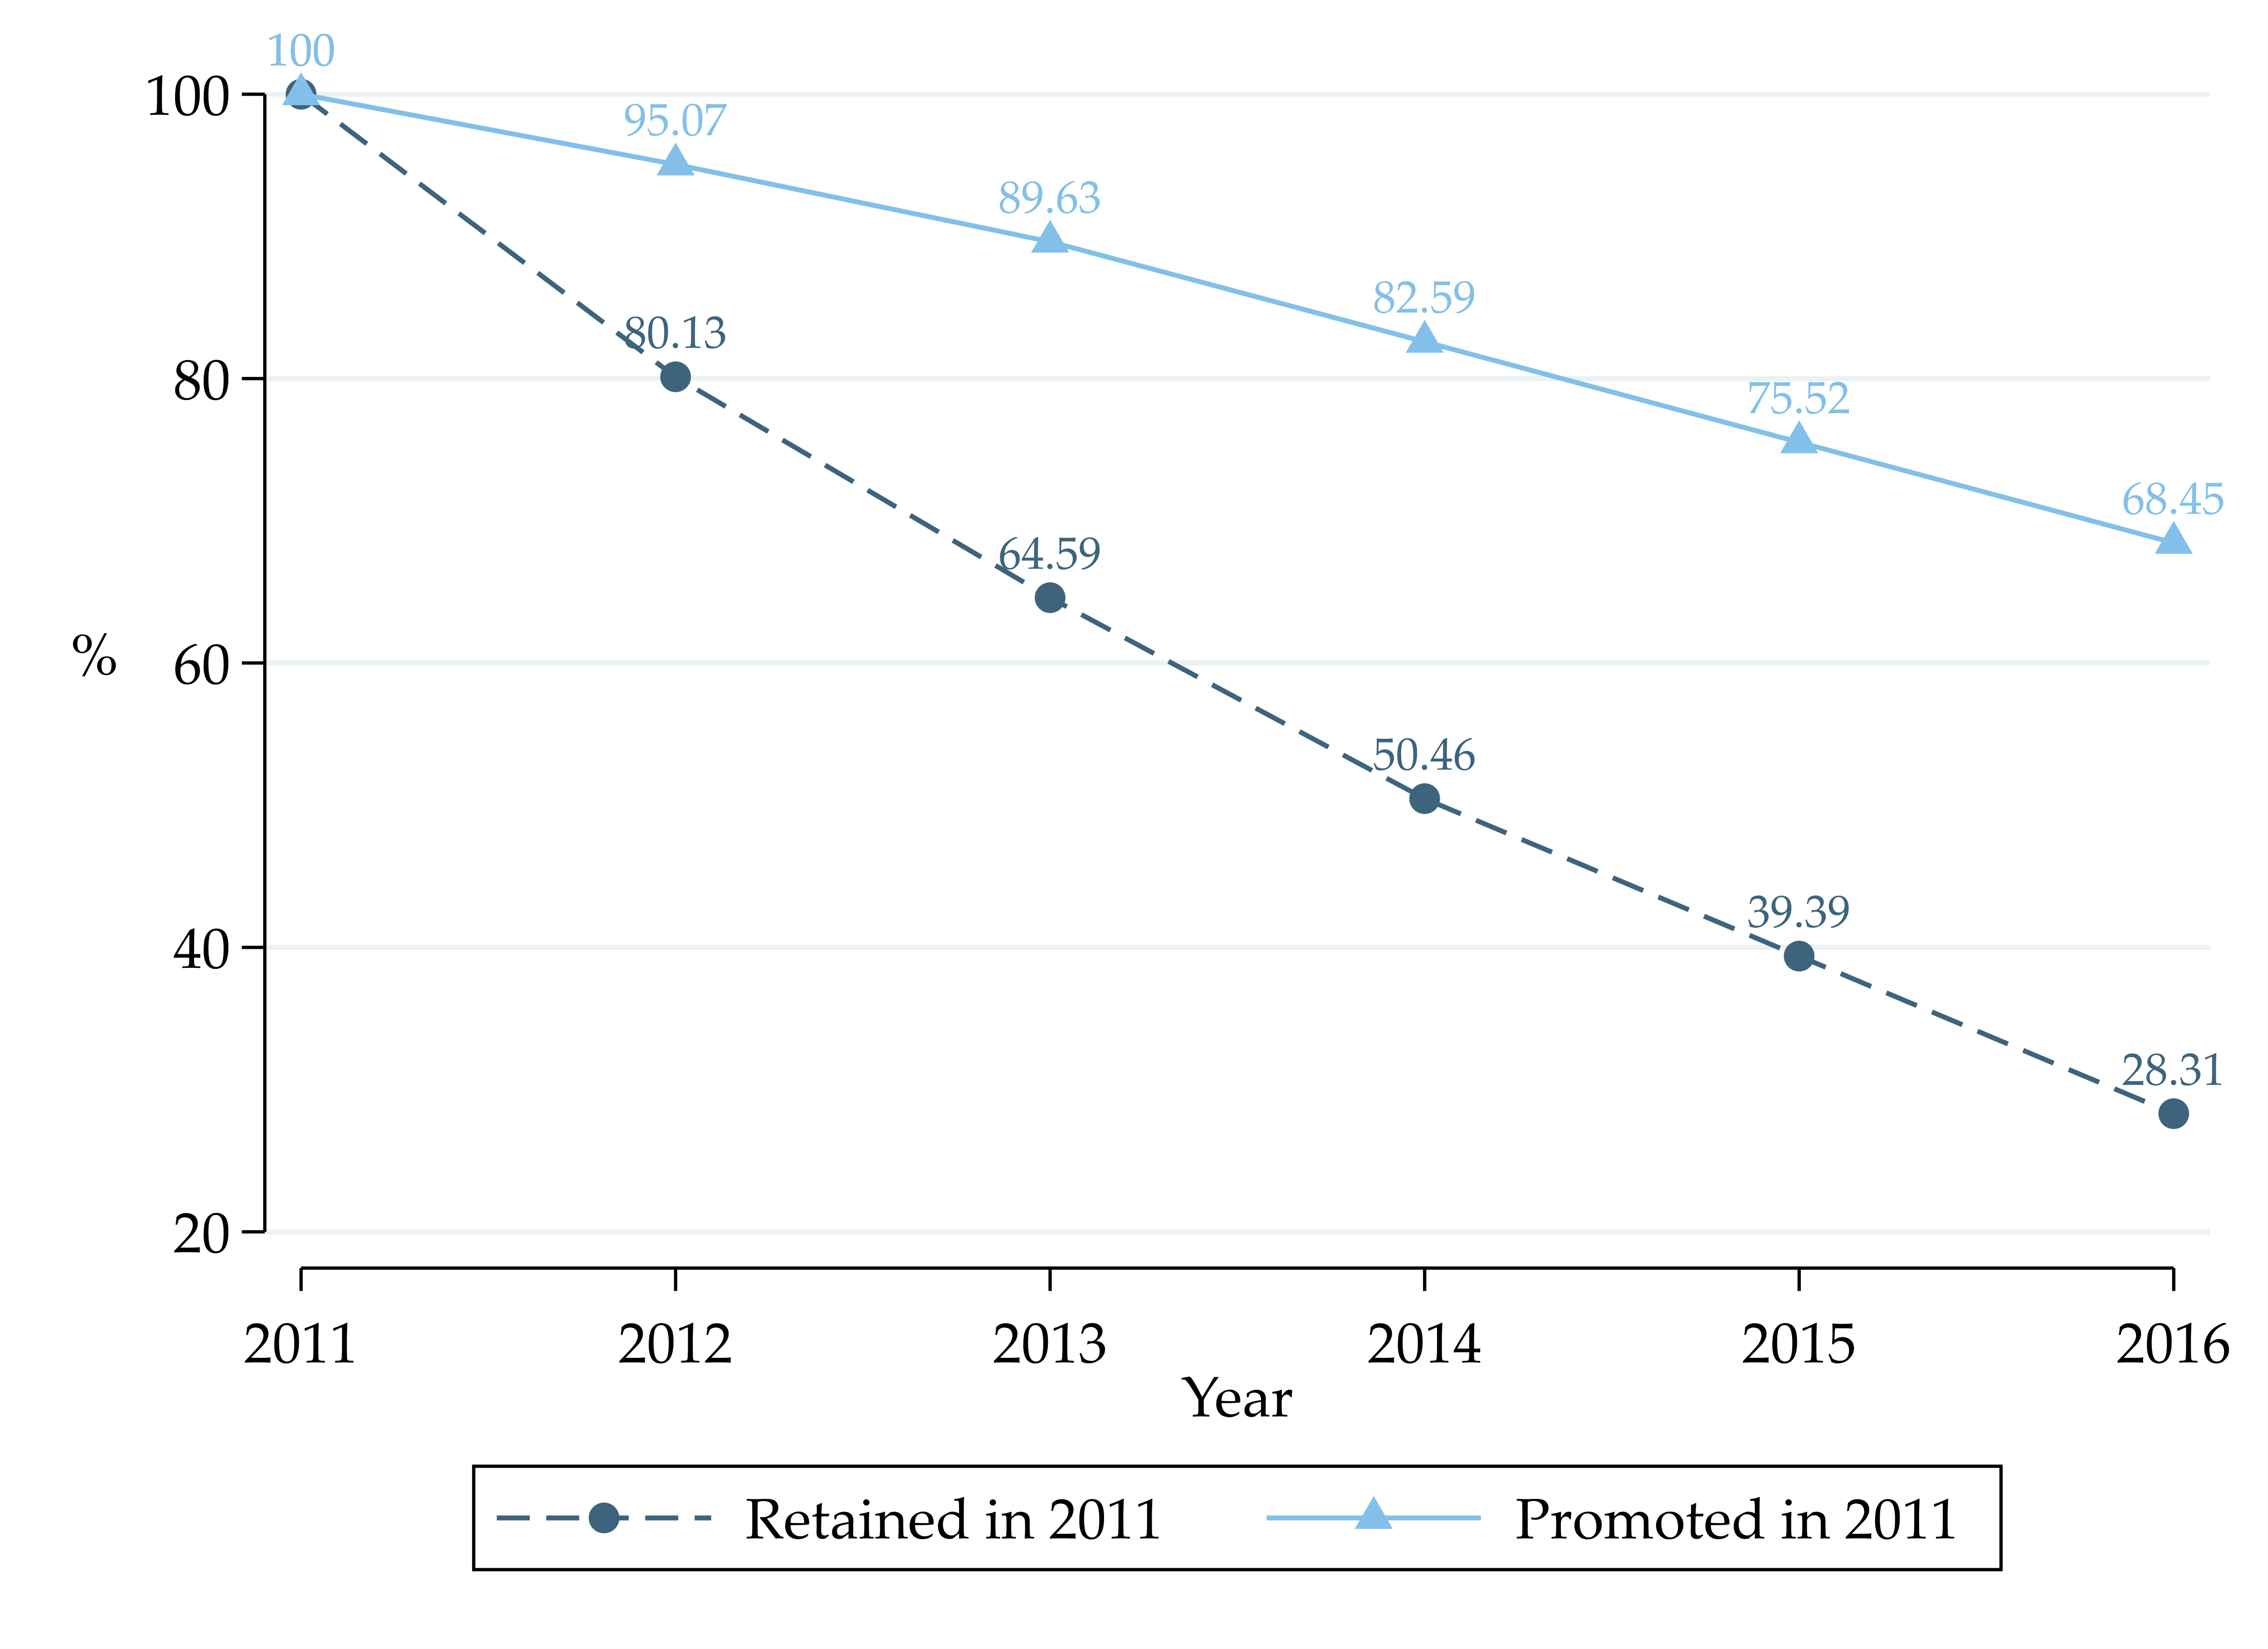
\includegraphics[width=0.8\textwidth]{DataWork/Output/Figures/fig5a-retention_grade6_dropout.png}
		\end{subfigure} 
		
		\begin{subfigure}{\textwidth}
			\caption{Years of Completed Schooling of 2011 6\textsuperscript{th} Graders}
			\label{fig:retention_grade6_education}
			\centering
			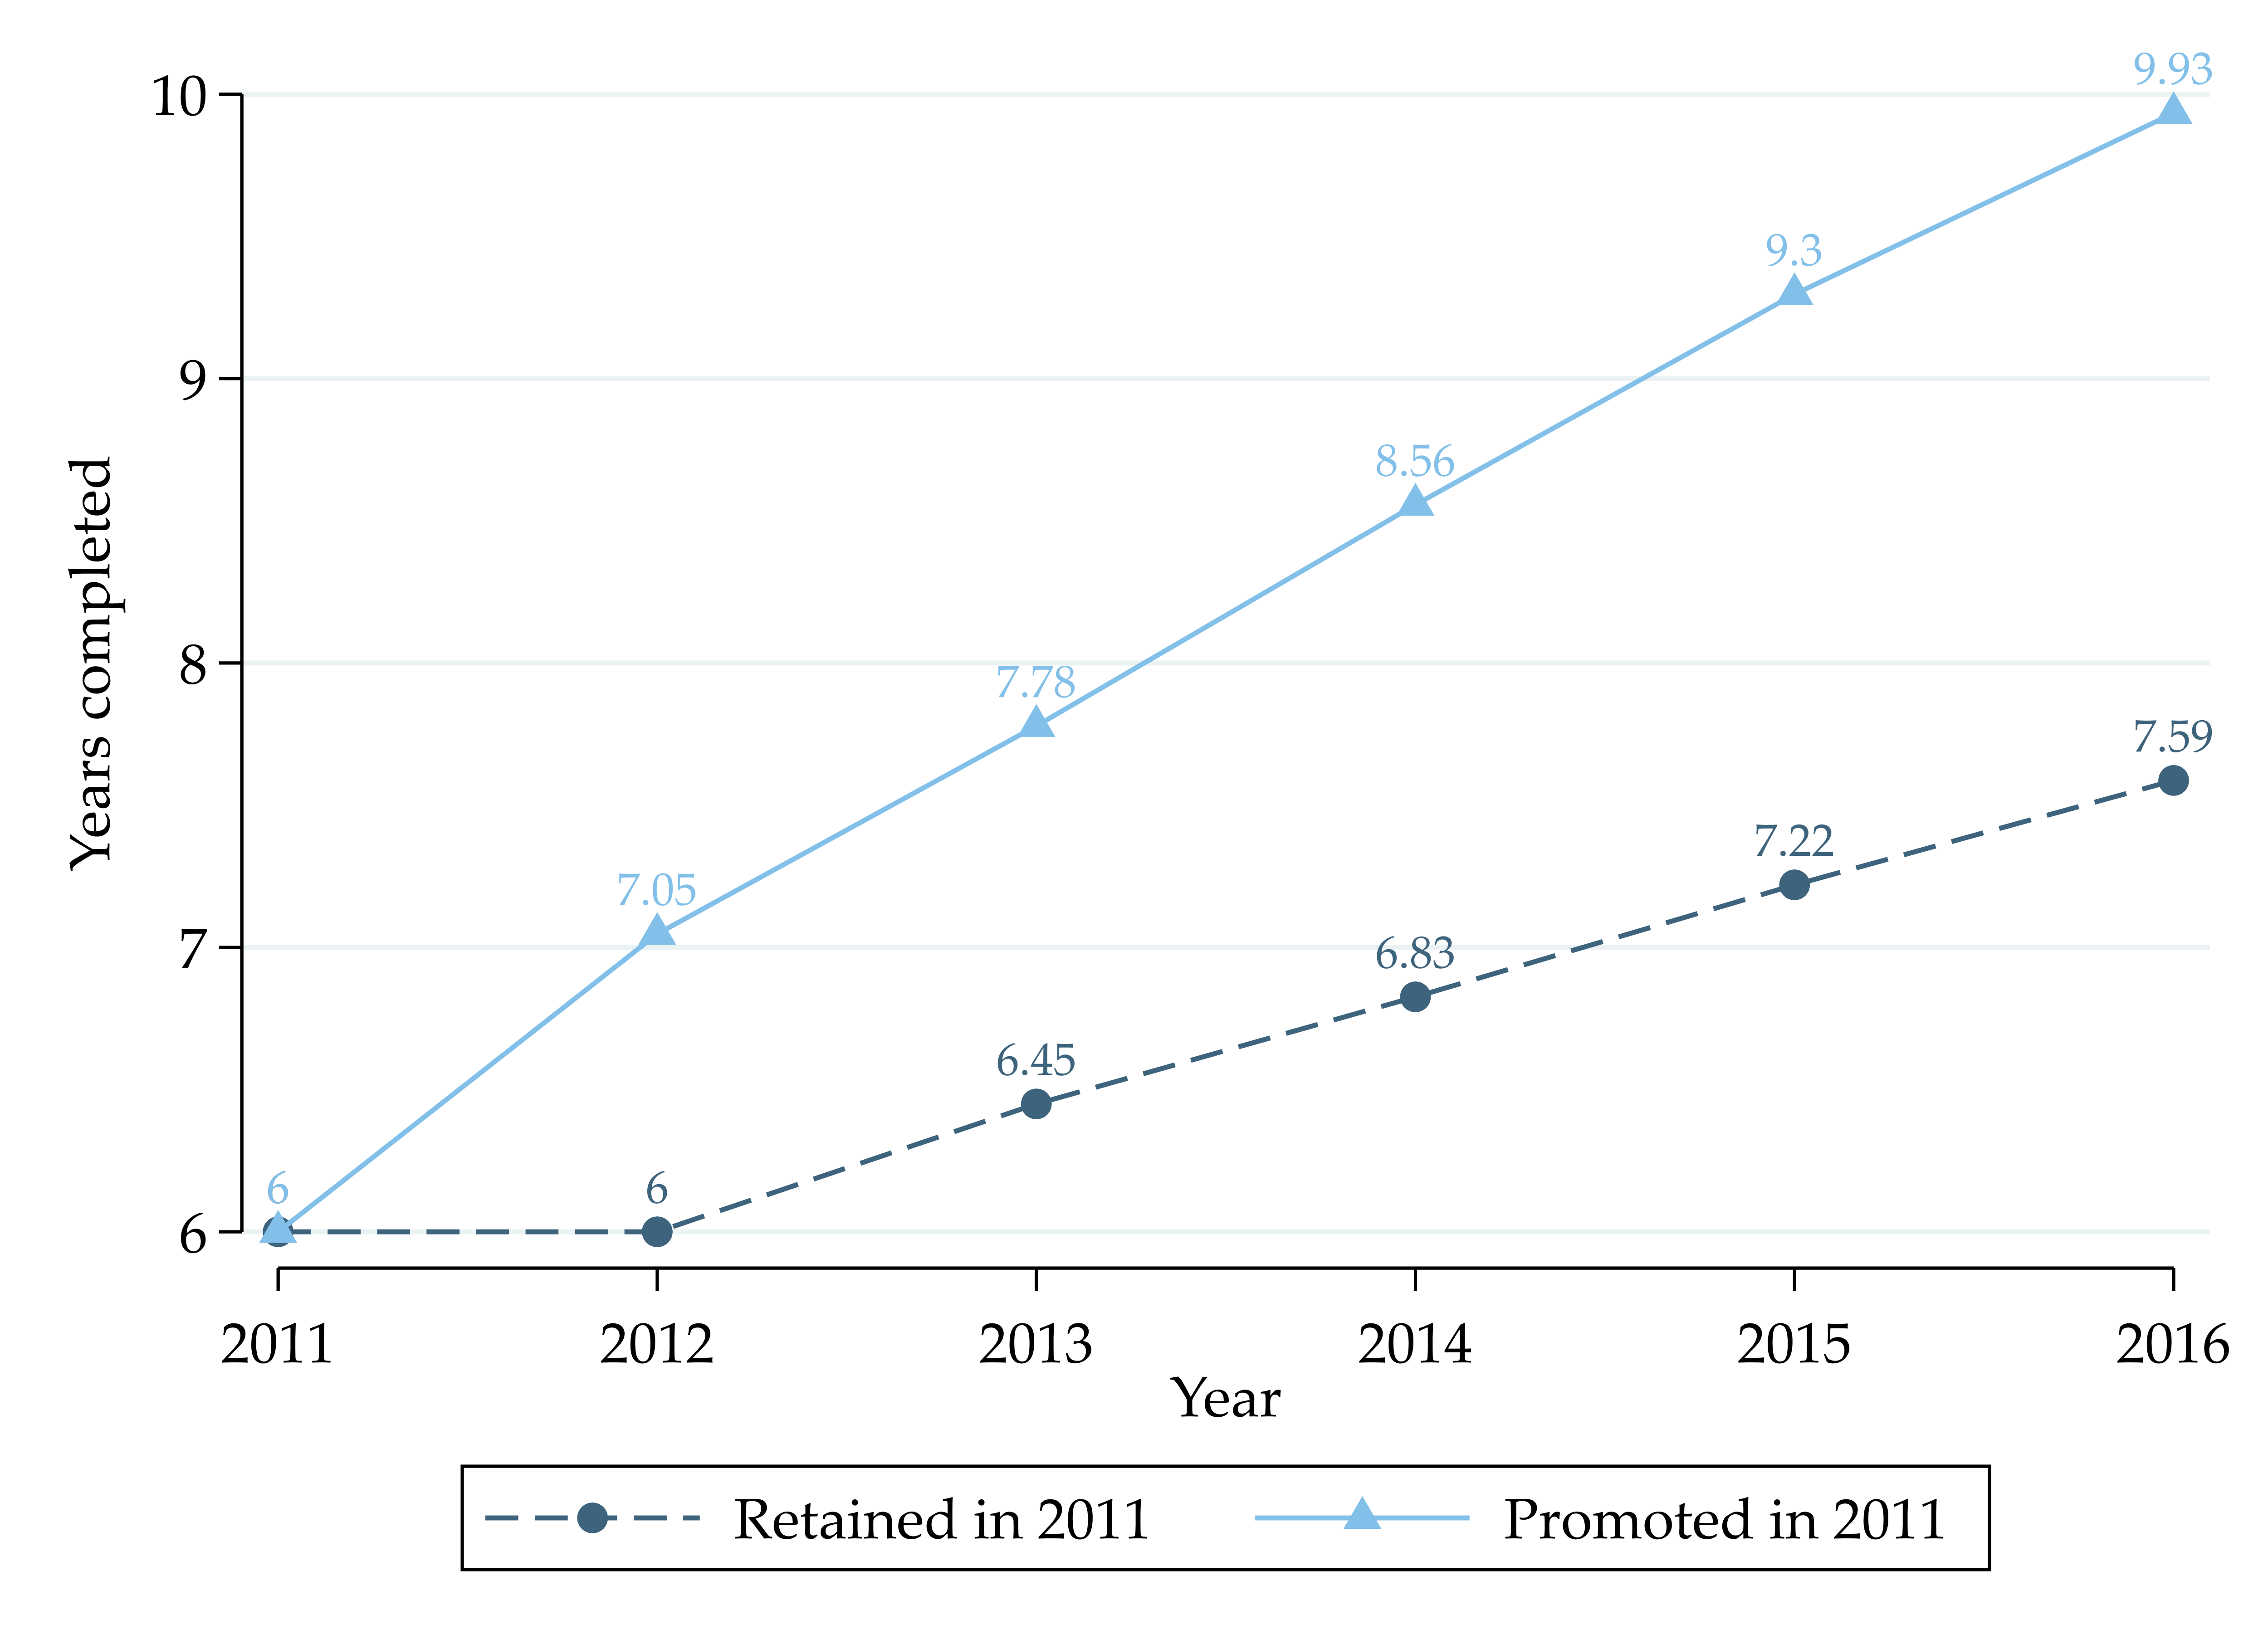
\includegraphics[width=0.8\textwidth]{DataWork/Output/Figures/fig5b-retention_grade6_education.png}
		\end{subfigure}  
		
		\begin{minipage}{0.825\textwidth}
			\small{\textit{Notes:} The points in Panel (a) show the percentage of 6\textsuperscript{th} graders in 2011 who were enrolled in any grade (6\textsuperscript{th} or higher) in the following years, up to 2016. Panel (b) shows the average years of completed schooling of students who were enrolled in 6\textsuperscript{th} grade in 2011 by each following year, up to 2016. The sample is fully representative of students of public schools in Rio Grande do Norte (N = 73,010) and is split between those who were promoted in 2011 and those who were retained in 2011. Data from 2011-2017 censuses.}
		\end{minipage}
	\end{figure}
	
	\section{Potential Mechanisms} \label{sec:mechanism}
	
	The results show that PIP had substantial impact on student learning and progression in Grade 6. In this section we explore the mechanisms through which the intervention may have affected these outcomes. As discussed in Section \ref{sec:pip}, there are three different components of the intervention, namely: 1) teacher autonomy, 2) technical support through mentors, and 3) financial support.
	
	We hypothesize two main channels by which PIP can improve student outcomes: 
	\begin{itemize}
		\item Increasing teacher motivation by providing them with the autonomy and resources to develop their own project with technical support;
		\item Implementation of innovative projects in the schools, increasing students' motivation and skills.
	\end{itemize}
	
	Teacher autonomy over the design and use of the grant likely affects student outcomes through both channels: 1) it may crowding in teacher intrinsic motivation and affect teaching quality as well as 2) lead to better tailored projects. The technical assistance was aimed at ensuring good implementation of projects. Both channels in turn may foster student-teacher interactions, which may strengthen the impacts of the project by developing students' socio-emotional skills. The results presented in the previous section indicate that these elements are particularly relevant in Grade 6, the transition between primary and lower secondary education. 
	
	In this section we explore which of the channels were affected and potential complementarities between project components. However, we cannot tell apart the relative importance of the different components in affecting these channels as the same package was offered to all treatment schools. 
	
	\subsection{Teacher Motivation} \label{sec:turnover}
	
	An important channel through which the PIP might have impacted students' outcomes is by improving teacher motivation. PIP allowed substantial autonomy for teachers to develop a project and provided funding to enable the implementation of the planned activities. In addition to leading to more relevant projects for the teachers, the autonomy in itself may have affected teachers' motivation and engagement with students, which in turn can affect student outcomes. We do not directly observe teachers' motivation in our data. To document whether the PIP might have affected teachers' commitment and motivation, we look at teacher turnover as a proxy.\footnote{To define teacher turnover, we track teachers across years in the school census. The outcome is a dummy of whether a teacher is in the same school in two consecutive years. The dummy is one if a teachers is still teaching in the same school (in any grade) and zero otherwise.} ITT estimates shown in Panel A of Table \ref{tab:turnover_teacherlevel} suggest the project increased the probability of a teacher staying in the same school the following year by 6.4 pp (9.3\% more compared to the control mean of 69.1\%) in 6\textsuperscript{th} grade. The higher teacher turnover in control schools is driven by more teachers leaving to other schools. They do not leave the education system (e.g., due to migration, retirement, or leaving the public system) more than in treatment schools. We interpret this result as suggestive evidence that part of project's success in Grade 6 was achieved by increasing commitment among these teachers. 
	
	Panel B in Table \ref{tab:turnover_teacherlevel} suggests that the results are concentrated in schools with higher teacher turnover rates at baseline. `High teacher turnover' is defined at the grade level as a school having a turnover rate above the sample median of that grade before the intervention.\footnote{To define `high teacher turnover' schools at baseline we calculate the proportion of teachers who leave a school between the 2015 and 2016 school year. `High teacher turnover' is defined as a dummy, which takes the value one if the proportion of teachers leaving that school is above the median turnover distribution for schools treated in that grade} The median for schools treated at 6\textsuperscript{th} grade is 33.33\%.\footnote{Most 5\textsuperscript{th} grade schools have only one teacher and there median turnover rate is zero.} We leverage this finding to document whether teacher turnover is a likely mechanism driving the learning results. We find that the impacts on learning are also concentrated in schools with high teacher turnover at baseline. Impacts on learning for this group approaches 0.28 SD (Table  \ref{tab:het_turnover}).   
	
	\vfill
	
	% Impact on teacher turnover
	\begin{table}[ht!]
		\caption{Impact on Probability of Teacher Staying in the Same School}
		\label{tab:turnover_teacherlevel}
		\centering
		\begin{adjustbox}{max width=\textwidth}
			\begin{tabular}{lDDDD} \hline \hline
				&(1) &(2) &(3) &(4)                                                                                                                                              \\                       
&All &5th &6th &10th                                                                                                                                             \\             \hline
\addlinespace[0.25em] \multicolumn{5}{c}{\textbf{Panel A -- Overall impact}}                             \\[0.25em] \hline
\addlinespace[0.5em]             Treatment   &       0.036         &      -0.064         &       0.064\sym{*}  &       0.033         \\              &     (0.029)         &     (0.065)         &     (0.037)         &     (0.049)         \\    \addlinespace[0.5em] Number of observations&        1882         &         189         &         784         &         909         \\  Number of clusters&         277         &          95         &         104         &          78         \\  \addlinespace[0.5em] Mean dep.\ var.\ control group&       0.709         &       0.761         &       0.691         &       0.714         \\  SD dep.\ var.\ control group&       0.454         &       0.428         &       0.463         &       0.452         \\                                                                                                                                [0.75em] \hline
\addlinespace[0.25em] \multicolumn{5}{c}{\textbf{Panel B -- Impact by turnover at baseline}} \\[0.25em] \hline
\addlinespace[0.5em]                      Treatment   &      -0.016         &                     &       0.014         &      -0.038         \\              &     (0.042)         &                     &     (0.046)         &     (0.064)         \\    Treatment $\times$ High teacher turnover rate at baseline&       0.095\sym{*}  &                     &       0.104         &       0.139         \\              &     (0.058)         &                     &     (0.074)         &     (0.092)         \\    High teacher turnover rate at baseline&      -0.109\sym{***}&                     &      -0.127\sym{**} &      -0.115\sym{*}  \\              &     (0.038)         &                     &     (0.050)         &     (0.058)         \\    \addlinespace[0.5em] Constant&       0.776\sym{***}&                     &       0.756\sym{***}&       0.780\sym{***}\\              &     (0.025)         &                     &     (0.032)         &     (0.036)         \\    \addlinespace[0.75em] \multicolumn{5}{l}{\textit{Total effect on schools with high turnover at baseline:} Treatment $+$ Treatment $\times$ high-turnover dummy} \\ \hspace{10pt} $\sum \hat{\beta}$&       0.079         &                     &       0.118         &       0.101         \\  \hspace{10pt} P-value&       0.048         &                     &       0.043         &       0.131         \\  \addlinespace[0.75em] \multicolumn{5}{l}{\textit{Unconditional mean of the dependent variable in the control group:}} \\ \hspace{10pt} Schools with high turnover at baseline&       0.664         &                     &       0.626         &       0.649         \\  \hspace{10pt} Schools with low turnover at baseline&       0.775         &                     &       0.762         &       0.786         \\                                                                                                                         \hline
\hline \\ [-1.8ex]
				\multicolumn{5}{@{}p{1.12\textwidth}}{\footnotesize \textit{Notes}: \sym{*}Significant at 10\%. \sym{**}Significant at 5\%. \sym{***}Significant at 1\%. Data are from Rio Grande do Norte 2016 and 2017 teacher censuses. Unit of observation: teacher. $\sum \hat{\beta}$ is the sum of the treatment effect with the interaction variable coefficient. The p-value refers to the null hypothesis $\sum \hat{\beta} = 0$. All regressions are linear probability model with strata (i.e., region and grade) fixed effects. Standard errors clustered at the school level in parentheses. Note that the coefficient on the high-turnover dummy at baseline for 5\textsuperscript{th} grade is not identified because the median itself is equal to 0. This is due to the fact that, in most schools, 5\textsuperscript{th} grade has only one teacher, thus the school turnover rate variable is either equal to 0 or 1.}
			\end{tabular} 
		\end{adjustbox}
	\end{table}
	%
	
	% Impact on test scores and learning by teacher turnover
	\begin{table}[ht!]
		\caption{Impact on Student Learning and Progression by Teacher Turnover at Baseline}
		\label{tab:het_turnover}
		\centering
		\begin{adjustbox}{max width=\textwidth}
			\begin{tabular}{lcccc} \hline \hline
				&\multicolumn{1}{c}{\textit{Learning}}   &\multicolumn{3}{c}{\textit{Progression}} \\           
 \cmidrule(lr){2-2}                                       \cmidrule(lr){3-5}                                                        
&(1)                                                                     &(2)    &(3)     &(4)                                         \\           
&Average                                                                 &Passed &Dropped &Retained                        \\           
&test score                                                      &       &out     &                                        \\ \hline
\multicolumn{5}{c}{\textbf{All schools}}                                                                                       \\ \hline
                    Treatment   &      -0.059         &       0.081\sym{**} &       0.006         &      -0.086\sym{***}\\              &     (0.075)         &     (0.037)         &     (0.025)         &     (0.029)         \\    Treatment $\times$ High teacher turnover at baseline&       0.132         &      -0.063         &      -0.023         &       0.087\sym{**} \\              &     (0.093)         &     (0.046)         &     (0.031)         &     (0.035)         \\    High teacher turnover at baseline&      -0.188\sym{***}&       0.046         &       0.016         &      -0.062\sym{**} \\              &     (0.072)         &     (0.034)         &     (0.026)         &     (0.028)         \\    \addlinespace[0.5em] Constant&       0.118\sym{*}  &       0.569\sym{***}&       0.162\sym{***}&       0.269\sym{***}\\              &     (0.066)         &     (0.025)         &     (0.020)         &     (0.023)         \\    \addlinespace[0.75em] Number of observations&       11794         &       16159         &       16169         &       16159         \\  Number of clusters&         228         &         239         &         239         &         239         \\  \addlinespace[0.75em] \multicolumn{5}{l}{\textit{Total effect:} Treatment $+$ Treatment $\times$ High teacher turnover at baseline} \\ \hspace{10pt} $\sum \hat{\beta}$&       0.073         &       0.017         &      -0.018         &       0.000         \\  \hspace{10pt} P-value&       0.176         &       0.541         &       0.328         &       0.982         \\                                                                                                                                                          \hline
\multicolumn{5}{c}{\textbf{6th  grade -- Lower secondary schools}}                                 \\ \hline
                    Treatment   &       0.016         &       0.079\sym{*}  &      -0.025         &      -0.054         \\              &     (0.080)         &     (0.043)         &     (0.027)         &     (0.037)         \\    Treatment $\times$ High teacher turnover at baseline&       0.261\sym{**} &      -0.023         &      -0.043         &       0.066         \\              &     (0.119)         &     (0.058)         &     (0.037)         &     (0.053)         \\    High teacher turnover at baseline&      -0.200\sym{***}&      -0.046         &       0.045         &       0.000         \\              &     (0.063)         &     (0.040)         &     (0.032)         &     (0.034)         \\    \addlinespace[0.5em] Constant&       0.062         &       0.613\sym{***}&       0.115\sym{***}&       0.272\sym{***}\\              &     (0.039)         &     (0.029)         &     (0.024)         &     (0.023)         \\    \addlinespace[0.75em] Number of observations&        4333         &        5261         &        5265         &        5261         \\  Number of clusters&          94         &          98         &          98         &          98         \\  \addlinespace[0.75em] \multicolumn{5}{l}{\textit{Total effect:} Treatment $+$ Treatment $\times$ High teacher turnover at baseline} \\ \hspace{10pt} $\sum \hat{\beta}$&       0.276         &       0.055         &      -0.067         &       0.012         \\  \hspace{10pt} P-value&       0.002         &       0.186         &       0.008         &       0.752         \\  \hline                                                                                                                                           \hline

				\multicolumn{5}{@{}p{0.985\textwidth}}{\footnotesize \textit{Notes}: \sym{*}Significant at 10\%. \sym{**}Significant at 5\%. \sym{***}Significant at 1\%. `Average test score' is the average of standardized test scores in math, Portuguese, human and social science. Student-level data on progression are from Rio Grande do Norte census. Teacher data are from Rio Grande do Norte 2016 and 2017 teacher censuses. Unit of observation: student. $\sum \hat{\beta}$ is the sum of the treatment effect with the interaction variable coefficient. The p-value refers to the null hypothesis $\sum \hat{\beta} = 0$. All regressions are OLS with strata (i.e., region and grade) fixed effects. The coefficient on learning is expressed in terms of standard deviations from the control group. The coefficients on progression are expressed in terms of percentage points. Standard errors clustered at the school level in parentheses.}
			\end{tabular} 
		\end{adjustbox}
	\end{table}
	%
	
	\FloatBarrier
	\clearpage
	\subsection{Implementation of Innovative Projects} \label{sec:innovative_projects}
	
	The impact of implementation of the innovative sub-projects may be due to projects being tailored to school specific needs or they may just good in their own right; the latter would for example mean they would have had the same impact if different sub-projects were rolled out randomly. We are not able to tell these two channels apart. Neither can we separate the impact of implementing the sub-projects from the impacts obtained through increasing teacher motivation.   
	
	We however explore the importance of complementing the teacher motivation with implementing the sub-projects. We do this by testing whether the motivational impacts on 6\textsuperscript{th} grade teachers also spill over to the other grades they teach, where they do not implement the innovative projects. According to census data, 90.43\% of 6\textsuperscript{th} grade teachers teach 7\textsuperscript{th} grade in the treatment (in the control), 81.76\% in 8\textsuperscript{th} grade, and 73.21\% in 9\textsuperscript{th} grade.\footnote{The percentage is balanced between treatment and control schools.} Panel A Table \ref{tab:spillover_other_grades} reports teacher turn-over in the remaining grades of 6\textsuperscript{th} grade school only. We find a significant increase (at the 5\% level) in the probability of a teacher staying in the same school also in 7\textsuperscript{th} grade (7.8 pp). Coefficients for 8\textsuperscript{th} and 9\textsuperscript{th} grade are smaller and not precisely estimated.
	
	We compare student level outcomes for the same 6\textsuperscript{th} grade schools, in the remaining lower-secondary grades. We only have access to data on student progression in other grades, the standardized test was not implemented in 7\textsuperscript{th} grade. The results on student progression rates suggest that the impact of the PIP on teacher commitment did not spill over to students of more advanced grades.\footnote{The results with grade level data from SIGEduc are very similar. See Online Appendix.} The lack of spillovers suggests that even though the project may have affected teacher motivation, this alone was not sufficient to also affect student outcomes in other grades: positive results in 6\textsuperscript{th} grade are likely driven by the combination of increased motivation with the other project components. These results are in line with recent evidence on complementarities between school inputs (in our case, the project activities and materials) and teacher incentives (or motivation) \citep{mbiti2019inputs}. 
	
	% Spillover to other grades
	\clearpage
	\null
	\vfill
	\begin{table}[ht!]
		\caption{Spillover to Other Grades in 6\textsuperscript{th} Grade Treated Schools}
		\label{tab:spillover_other_grades}
		\centering
		\begin{adjustbox}{max width=\textwidth}
			\begin{tabular}{lCCCC} \hline \hline
				&(1) &(2) &(3) &(4)                                                                                                                     \\         
&6th &7th &8th &9th                                                                                                                     \\ \hline  
\multicolumn{5}{c}{\textbf{Panel A -- Teacher level}}                                                   \\ [0.25em]
&\multicolumn{4}{c}{\textit{Probability of teacher staying in the same school}} \\ \hline  
           Treatment   &       0.064\sym{*}  &       0.078\sym{**} &       0.044         &       0.049         \\              &     (0.037)         &     (0.037)         &     (0.037)         &     (0.039)         \\    Number of observations&         784         &         792         &         759         &         682         \\  Number of clusters&         104         &         103         &          99         &          93         \\  Mean dep.\ var.\ control group&       0.691         &       0.697         &       0.691         &       0.688         \\  SD dep.\ var.\ control group&       0.463         &       0.460         &       0.463         &       0.464         \\  \hline                                                                                                                       \\ \hline  
\multicolumn{5}{c}{\textbf{Panel B -- Student level}}                                                   \\ [0.25em]
&\multicolumn{4}{c}{\textit{Probability of student being promoted}}                     \\ \hline  
           Treatment   &       0.070\sym{**} &       0.014         &      -0.005         &       0.010         \\              &     (0.031)         &     (0.032)         &     (0.029)         &     (0.036)         \\    Number of observations&        5490         &        4465         &        3294         &        2883         \\  Number of clusters&         104         &         103         &          99         &          93         \\  Mean dep.\ var.\ control group&       0.587         &       0.669         &       0.809         &       0.778         \\  SD dep.\ var.\ control group&       0.492         &       0.471         &       0.393         &       0.416         \\  \hline
&\multicolumn{4}{c}{\textit{Probability of student dropping out}}                       \\ \hline  
           Treatment   &      -0.043\sym{**} &      -0.029         &      -0.013         &      -0.038\sym{*}  \\              &     (0.018)         &     (0.018)         &     (0.018)         &     (0.022)         \\    Number of observations&        5494         &        4473         &        3303         &        2889         \\  Number of clusters&         104         &         103         &          99         &          93         \\  Mean dep.\ var.\ control group&       0.135         &       0.136         &       0.114         &       0.151         \\  SD dep.\ var.\ control group&       0.342         &       0.343         &       0.317         &       0.358         \\   \hline
&\multicolumn{4}{c}{\textit{Probability of student being retained}}                     \\ \hline  
           Treatment   &      -0.027         &       0.015         &       0.018         &       0.028         \\              &     (0.028)         &     (0.027)         &     (0.017)         &     (0.021)         \\    Number of observations&        5490         &        4465         &        3294         &        2883         \\  Number of clusters&         104         &         103         &          99         &          93         \\  Mean dep.\ var.\ control group&       0.277         &       0.195         &       0.077         &       0.071         \\  SD dep.\ var.\ control group&       0.448         &       0.396         &       0.266         &       0.257         \\  \hline                                                                                                                              \hline  
                                                                                                                                                                \\ [-1.8ex]
				\multicolumn{5}{@{}p{0.925\textwidth}}{\footnotesize \textit{Notes}: \sym{*}Significant at 10\%. \sym{**}Significant at 5\%. \sym{***}Significant at 1\%. Data are from Rio Grande do Norte 2016 and 2017 teacher and student censuses. Unit of observation: teacher in the first panel and student in the other panels. Sample: schools treated at 6\textsuperscript{th} grade. All regressions are linear probability model with strata (i.e., region) fixed effects. Standard errors clustered at the school level in parentheses.}
			\end{tabular} 
		\end{adjustbox}
	\end{table}
	\vfill
	% 
	
	\subsection{Socio-Emotional Skills}
	
	Another potential pathway for PIP having caused improved learning outcomes is through building student's socio-emotional skills. Several studies have shown the link between socio-emotional skills and learning outcomes (e.g., \citealp{heckman2001importance}; \citealp{almlund2011personality}; \citealp{lee2012effect}; \citealp{segal2013misbehavior}). Throughout the development of the projects, schools were encouraged to design an intervention that would change student-teacher interactions, and engage students by exposing them to learning opportunities outside the classroom, moving away from the traditional lecture-based teaching. As a consequence, resulting projects may have directly affected student socio-emotional skills. In addition, increasing teacher motivation and commitment may provide an indirect channel to improve socio-emotional skills.
	
	Table \ref{tab:socio_studentlevel} shows the ITT estimates on each of the Big Five personality traits. The indicators are standardized and the coefficients can be interpreted in terms of standard deviations. Pooling all grades, we find that the project had a positive and statistically significant effect on conscientiousness and extroversion.\footnote{The same robustness checks used for estimating the impact on learning outcomes can be seen in the Online Appendix.} However, in line with previous results, these are driven by the impact of PIP on 6\textsuperscript{th} graders. Among the Big Five, the trait of `conscientiousness' is commonly associated with acquisition of cognitive skills (\citealp{poropat2009meta}; \citealp{ivcevic2014predicting}). It encompasses traits such as self-control, organization, responsibility and perseverance. 
	
	% Impact on socio-emotional skills
	\vspace{20pt}
	\begin{table}[ht!]
		\caption{Impact on Socio-Emotional Skills}
		\label{tab:socio_studentlevel}
		\centering
		\begin{adjustbox}{max width=\textwidth}
			\begin{tabular}{lcccccc} \hline \hline
				&(1)                   &(2)                       &(3)          &(4)             &(5)          \\               
&Agreeableness &Conscientiousness &Extraversion &Neuroticism &Openness \\ \hline
\multicolumn{6}{c}{\textbf{All schools}}                                                       \\ \hline
           Treatment   &       0.048         &       0.115\sym{**} &       0.116\sym{**} &       0.037         &       0.058         \\              &     (0.056)         &     (0.054)         &     (0.054)         &     (0.047)         &     (0.054)         \\    Number of observations&        3560         &        3560         &        3560         &        3558         &        3560         \\  Number of clusters&         235         &         235         &         235         &         235         &         235         \\  Mean dep.\ var.\ control group&       4.413         &       4.331         &       4.199         &       4.007         &       4.105         \\  SD dep.\ var.\ control group&       0.975         &       1.053         &       0.777         &       0.738         &       0.970         \\     \hline
\multicolumn{6}{c}{\textbf{5th  grade -- Primary schools}}                     \\ \hline
           Treatment   &       0.023         &       0.094         &       0.049         &      -0.019         &      -0.061         \\              &     (0.097)         &     (0.095)         &     (0.097)         &     (0.073)         &     (0.094)         \\    Number of observations&        1296         &        1296         &        1296         &        1294         &        1296         \\  Number of clusters&          85         &          85         &          85         &          85         &          85         \\  Mean dep.\ var.\ control group&       4.468         &       4.359         &       4.287         &       4.040         &       4.193         \\  SD dep.\ var.\ control group&       1.049         &       1.108         &       0.851         &       0.738         &       0.997         \\  \hline
\multicolumn{6}{c}{\textbf{6th  grade -- Lower secondary schools}}     \\ \hline
           Treatment   &       0.078         &       0.173\sym{*}  &       0.208\sym{**} &       0.058         &       0.139         \\              &     (0.099)         &     (0.098)         &     (0.097)         &     (0.092)         &     (0.097)         \\    Number of observations&        1270         &        1270         &        1270         &        1270         &        1270         \\  Number of clusters&          87         &          87         &          87         &          87         &          87         \\  Mean dep.\ var.\ control group&       4.390         &       4.265         &       4.156         &       3.971         &       3.950         \\  SD dep.\ var.\ control group&       1.090         &       1.176         &       0.858         &       0.770         &       1.089         \\  \hline
\multicolumn{6}{c}{\textbf{10th grade -- Upper secondary schools}}     \\ \hline
           Treatment   &       0.042         &       0.069         &       0.085         &       0.082         &       0.110         \\              &     (0.091)         &     (0.080)         &     (0.079)         &     (0.075)         &     (0.080)         \\    Number of observations&         994         &         994         &         994         &         994         &         994         \\  Number of clusters&          63         &          63         &          63         &          63         &          63         \\  Mean dep.\ var.\ control group&       4.378         &       4.387         &       4.152         &       4.017         &       4.212         \\  SD dep.\ var.\ control group&       0.663         &       0.761         &       0.514         &       0.692         &       0.701         \\  \hline \hline \\ [-1.8ex]

				\multicolumn{6}{@{}p{1.175\textwidth}}{\footnotesize \textit{Notes}: \sym{*}Significant at 10\%. \sym{**}Significant at 5\%. \sym{***}Significant at 1\%. Unit of observation: student. All regressions are OLS with strata (i.e., region and grade) fixed effects. Standard errors clustered at the school level in parentheses. The coefficient are expressed in terms of standard deviations from the control group, while mean and standard deviation of the dependent variable refer to the raw values in the control group.}
			\end{tabular}
		\end{adjustbox}
	\end{table}
	
	\subsection{Understanding Heterogeneous Impacts by Grade}
	
	We presented the results to the mentors in a focus group discussion to shed light on what may be driving differences in impacts across grades. First, we found that mentors had more experience with teaching and implementing projects in lower grades, which may have resulted in the technical assistance being better tailored to these grades. Second, mentors stated that the project filled a clear gap faced by 6\textsuperscript{th} graders who experience a significant transition between levels of education. The key difference between these levels is that students in primary education have a single teacher, which allows for a close student-teacher relationship. These ties are weaker in lower secondary education, as students have multiple teachers (at least 5). The potential negative impact of this transition is well documented in the US and has been recently investigated in Brazil (\citealp{bedard2005middle}; \citealp{cook2006should}; \citealp{hanewald2013transition}; \citealp{dos2017mais}). \cite{dos2017mais} evaluate the impact of a pilot in municipal schools in Rio de Janeiro, Brazil, which expanded primary school to include  6\textsuperscript{th} grade. They find that having the 6\textsuperscript{th} grade in the primary school increases learning by 0.16 SD, and suggestive evidence that strengthening of student-teacher relationship mediated some of the effect on learning.  
	
	We compare administrative data to assess whether project implementation varied across the three grades. All treatment schools received similar levels of support from the SEEC team: all had an approved sub-project and were assigned a mentor who visited them regularly. Here we focus on the implementation of the planned activities by the schools throughout the year. We report three measures of implementation: i) obtaining the clearance certificate, which is a necessary requirement for schools to receive funding from any state level educational program\footnote{We indeed find that obtaining the clearance certificate is what most predicts rate of implementation (Table \ref{tab:predict_implementation}. We find that being assigned to receive the PIP increases the likelihood of schools obtaining the clearance certificate by 41 pp. This impact does not differ by grade (Table \ref{tab:clearance_certificate}).}; ii) percentage of project funds received by the end of the school year; and iii) whether a school implemented at least 70\% of the planned activities included in the work plan. We observe substantial difference in rates of implementation across the three grades (Figure \ref{fig:implementation_byGrade}). Each of the indicators shows higher rates of implementation in 6\textsuperscript{th} grade.\footnote{We do not observe any significant correlation between school characteristics at baseline and implementation (Table \ref{tab:predict_implementation}), however it is likely that implementation is endogenous to unobserved school quality and our outcomes of interest, therefore we refrain from comparing schools with high rates of implementation with low rates of implementation as these provide biased results.} 
	
	Taken together, Grade 6 schools may have perceived the project as being particularly relevant to smooth shocks observed around the transition from primary to lower secondary education. This may have led to better implementation in this grade. 
	
	\begin{figure}[ht!]
		\caption{Implementation by Grade}
		\label{fig:implementation_byGrade}
		\centering
		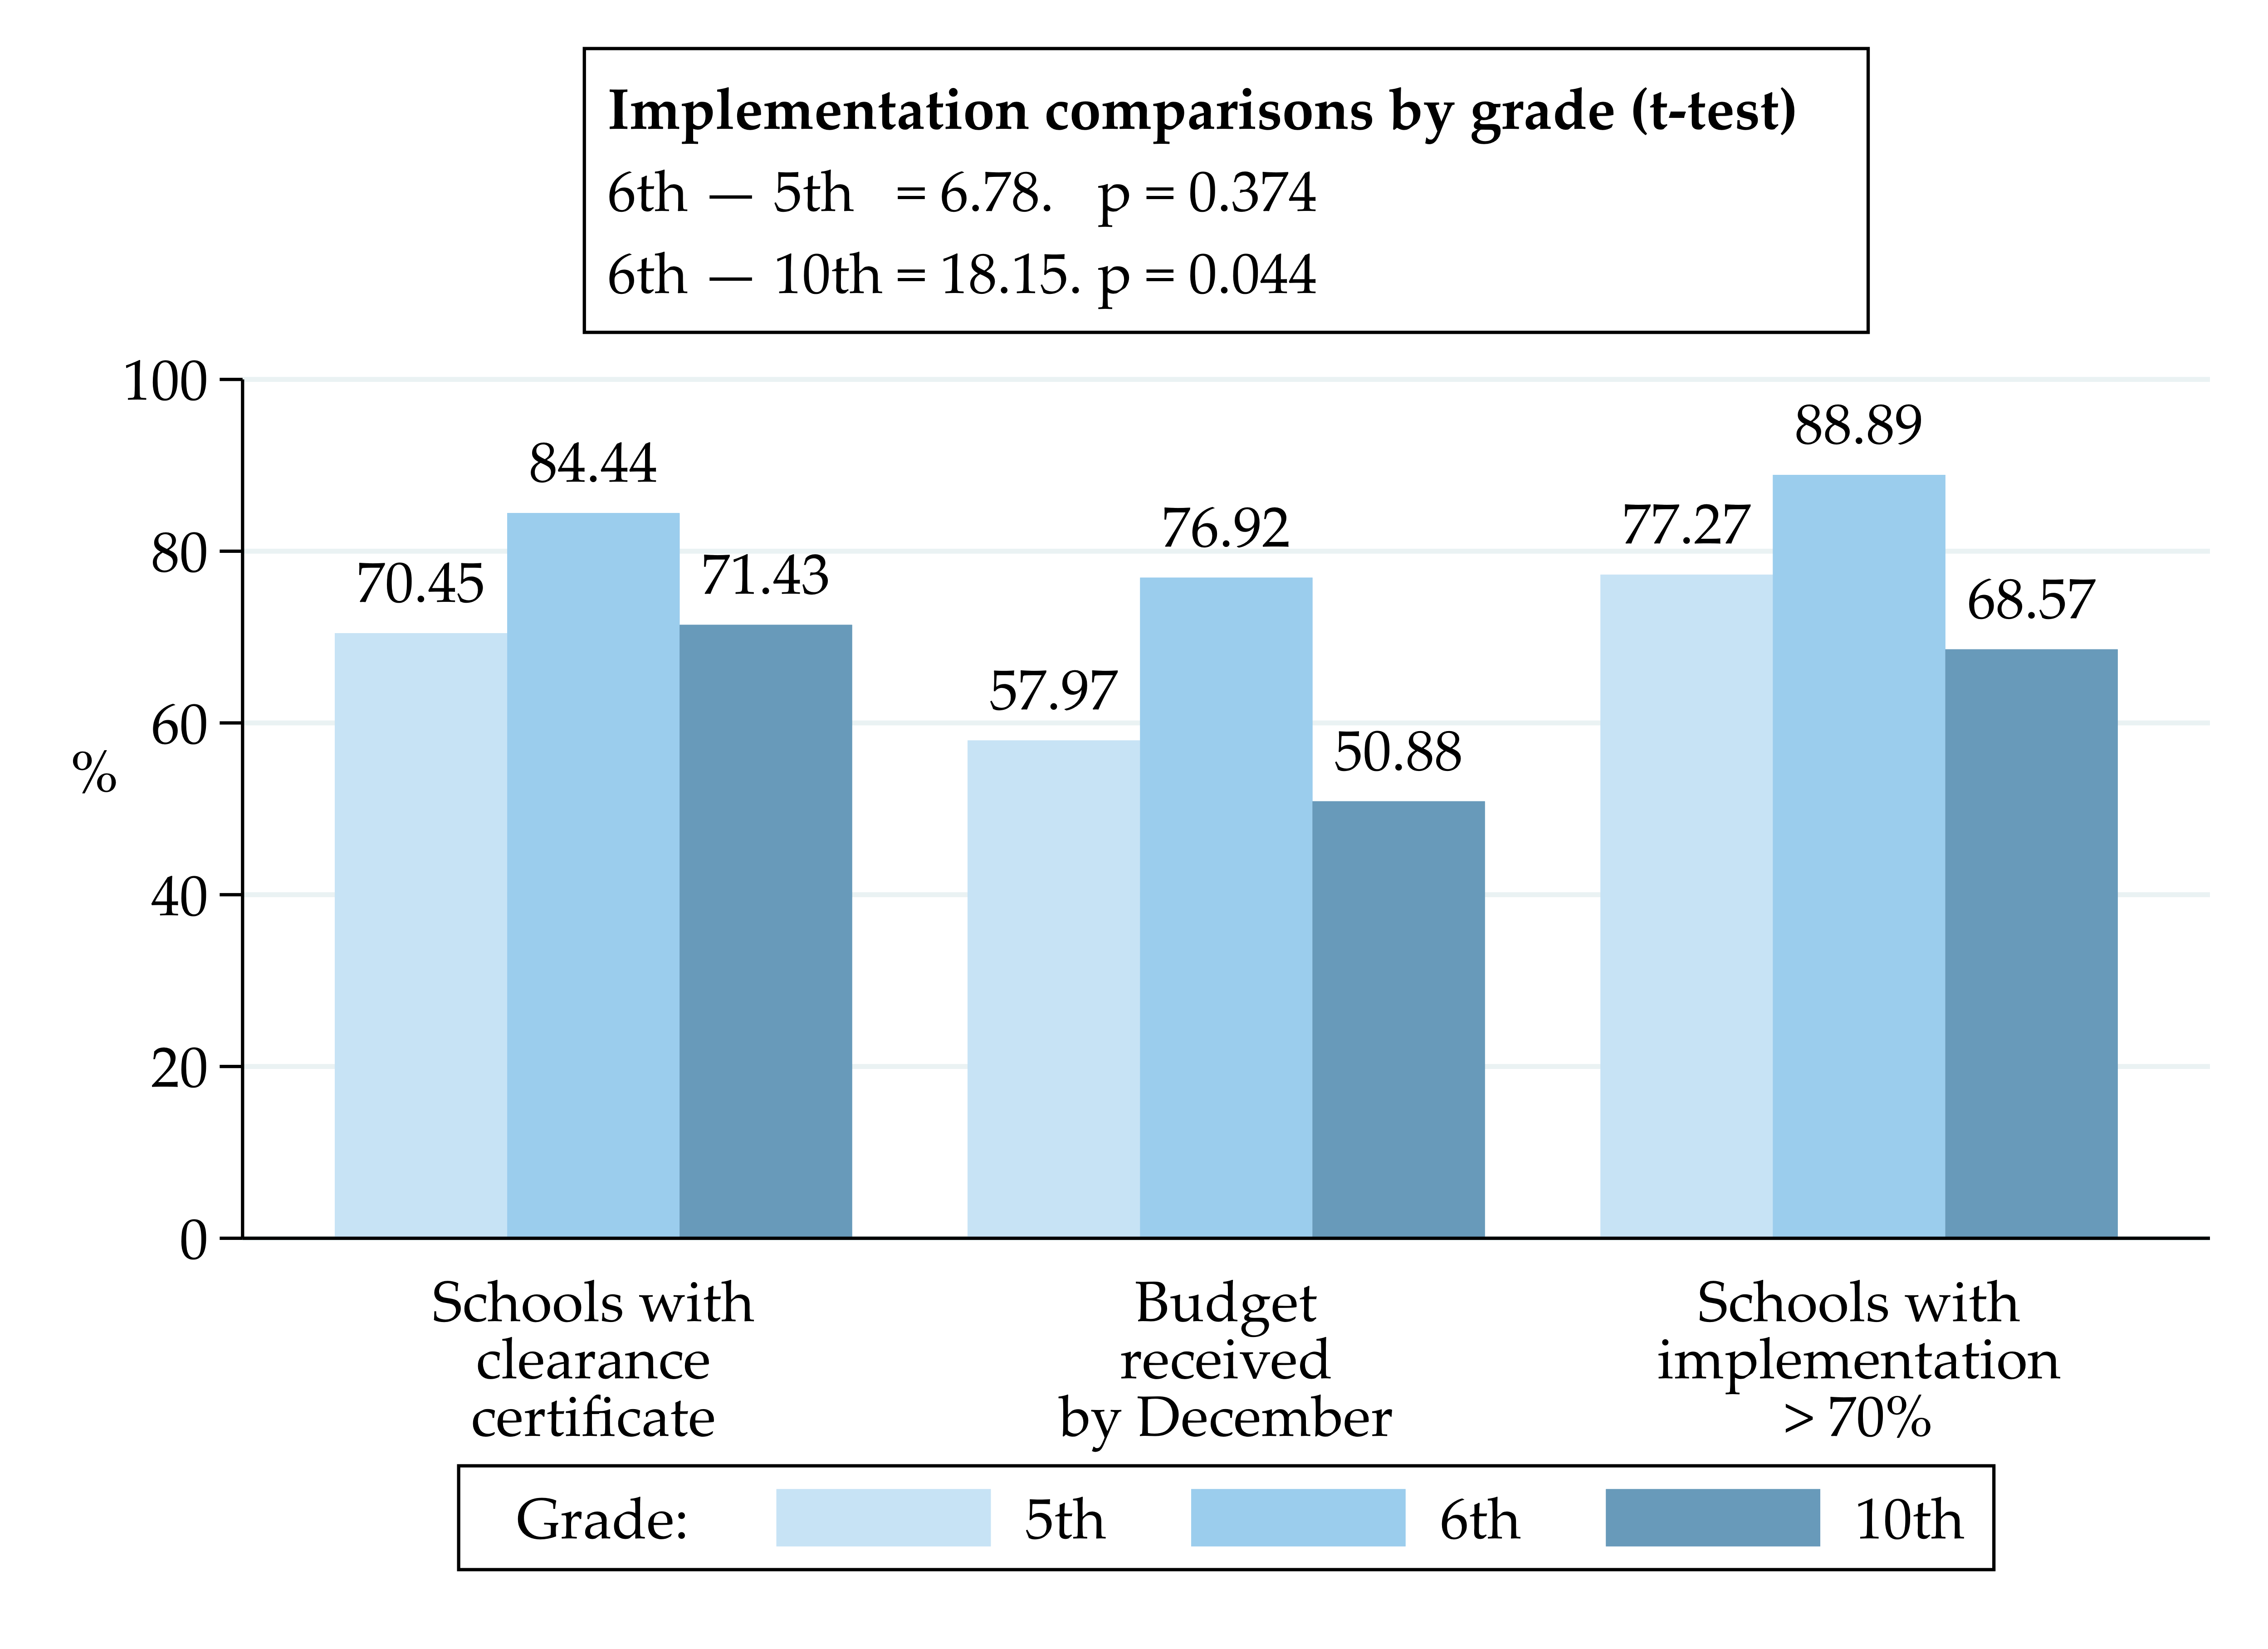
\includegraphics[width=14cm]{DataWork/Output/Figures/fig6-implementation_byGrade.png}
		\begin{minipage}{0.825\textwidth}
			\small{\textit{Notes:} `Implementation' is defined as the ratio of the number of activities that were implemented over the number of planned activities described in the work plan. Data are from State Secretary of Education. Sample: schools treated.}
		\end{minipage}
	\end{figure}
	\FloatBarrier
	
	\clearpage
	
	\section{Policy Analysis} \label{sec:policy}
	
	In this section we use the main results on learning and progression to produce back-of-the- envelope estimates for the impact of the program on school quality indicators and individuals' expected earnings
	
	\subsubsection*{Quality of Education} 
	
	Figure \ref{fig:itt_ProvaBrasil} shows that if students retain their learning gains over time, the impact of the PIP would suffice to close half of the knowledge gap between RN and the country's average by the end of Grade 9. 
	
	A top priority of state secretariats of education in Brazil is to show improvement in the Education Development Index. The index is computed as a geometric mean between grade passing rate and a simple average of math and Portuguese scores in the SAEB test.\footnote{See Appendix \ref{sec:ideb} for a detailed description of the index construction. As PIP was not implemented in all school grades, but only on 5\textsuperscript{th}, 6\textsuperscript{th} and 10\textsuperscript{th} grades, we need to make additional assumptions to compute an index applying the IDEB scale.} The index is re-scaled to vary from 0 to 5. Figure \ref{fig:itt_IDEB} shows the distribution of \textit{IDEB} across Brazilian states. We use the ITT estimates to compute the counterfactual distribution of \textit{IDEB} for RN. The strategy is described in more detail in Appendix \ref{sec:ideb}. ITT estimates suggest that the PIP would help RN state schools move upwards in the ranking by at least two positions.
	
	\subsubsection*{Expected Returns to Education} 
	
	We expect the intervention to impact labor market outcomes of the 6\textsuperscript{th} graders in the long-term through two channels: first via learning gains among those that stayed in school (productivity channel), and second via higher probability of remaining in school conditional on passing grade 6 (a combination of productivity effects with signaling or diploma effects). The first channel focuses on the improved quality of education, while the second reflects extra years of education among more knowledgeable students.
	
	Using the ITT effects of the PIP on learning as being approximately equal to 0.5 extra year of schooling, a back-of-the-envelop calculation suggests a NPV of 29,148.97 Brazilian Reais (BRL) -- or 7,287.24 US\$. The second channel is through the increase in student years of schooling conditional on passing Grade 6. Using school census data for RN between 2011 and 2017, we estimate that students that passed Grade 6 in 2011 had about 1.7 years of schooling in 2017 than students that failed Grade 6 in 2011. Given the PIP impacts on repetition rates in Grade 6 (23\%), we estimate that, on average, the 6\textsuperscript{th} graders receive about 0.4 extra years of schooling. A back-of-the-envelop calculation points to a NPV of 23,319.18 BRL (or 5,829.79 US\$). The full effect on expected earnings would then range from 7 to 13 thousand dollars or 28 to 52 Brazilian minimum wages. The data and methodology used for the calculations are described in Appendix \ref{sec:NPV}. 
	
	
	\section{Conclusion} \label{sec:conclude}
	
	The state schools of Rio Grande do Norte, one of the poorest states in Brazil, rank at the bottom of the Brazilian Development Education Index. To change this reality, the Secretariat of Education of RN designed an education policy to increase students' learning and reduce dropout rates, which mainly affect 6\textsuperscript{th} and 10\textsuperscript{th} grades. The program consisted of three key components: teacher autonomy to develop a work plan to tackle problems locally identified; technical assistance from supervisors assigned by the SEE to support teachers during the diagnostic and development of the work plan stages; and funding for schools to buy the pedagogical material necessary to implement the activities described in the work plan. 
	
	The results found in this paper suggest that the PIP had meaningful impacts on 6\textsuperscript{th} graders, a crucial school grade in the transition from primary to lower-secondary education. Given the budget allocated to basic education in Brazil and the challenges faced by public authorities to improve student learning, the experience in RN suggests that large impacts on school quality can be achieved in the short run, mostly through the reallocation of available inputs. Taking stock of the impacts it looks like that the complementary approach used by the PIP to tackle both incentive and supply-side constraints was key to secure high returns to treated schools and students. 
	
	The results have direct policy implications as they show that it is possible to obtain meaningful improvements in the quality of public education by combining teacher autonomy to increase motivation with technical assistance to strengthen local capacity. 
	
	
	
	%%%%%%%%%%%%%%%%%%%%%%%%%%%% BIBLIOGRAPHY %%%%%%%%%%%%%%%%%%%%%%%%%%%
	
	\clearpage
	\bibliography{references}
	
	%%%%%%%%%%%%%%%%%%%%%%%%%%%% APPENDIX TABLES AND FIGURES %%%%%%%%%%%%%%%%%%%%%%%%%%%
	\clearpage
	\appendix
	
	\section{Supplementary Figures and Tables}
	\setcounter{figure}{0}
	\setcounter{table}{0}
	\renewcommand{\thefigure}{A\arabic{figure}}
	\renewcommand{\thetable}{A\arabic{table}}
	\label{app:tables_figures}
	
	% IDEB by Participation and Treatment
	\null
	\vfill
	\begin{figure}[ht!]
		\caption{IDEB by Participation to Socio-Emotional Test and Treatment}
		\label{fig:predict_participation}
		\centering
		
		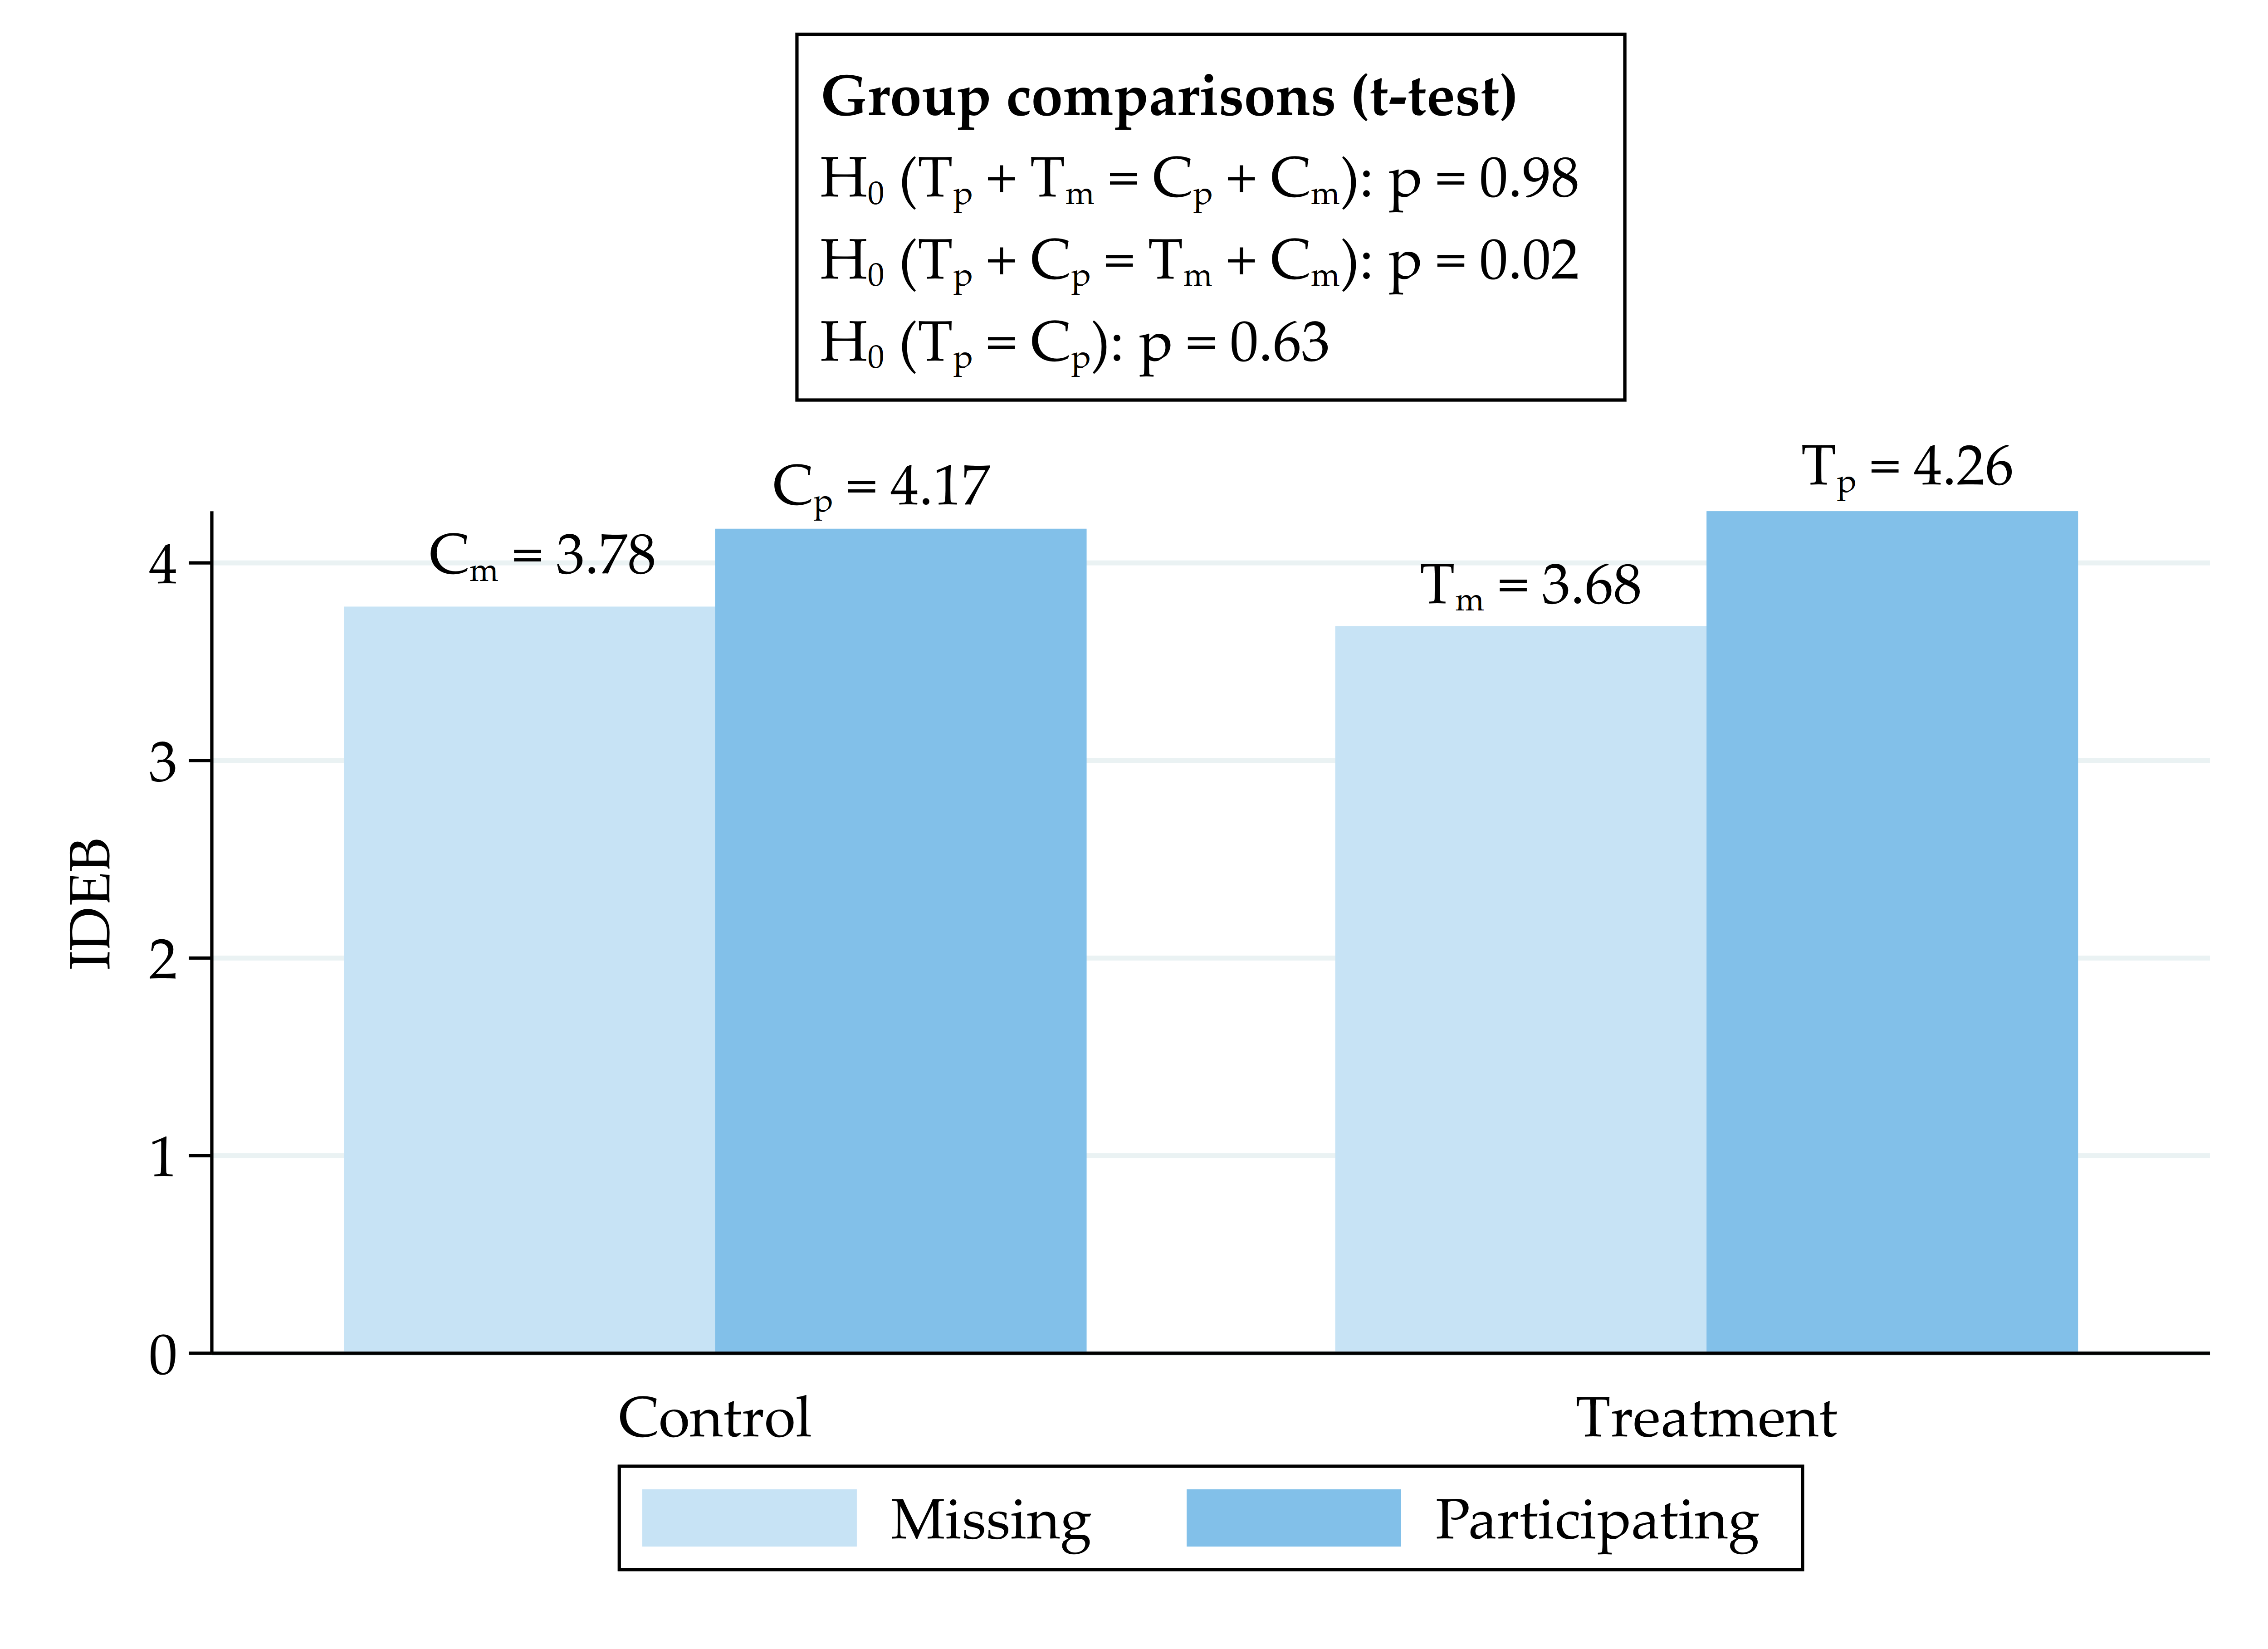
\includegraphics[width=14cm]{DataWork/Output/Figures/figA1_predict_participation.png}
		
		\noindent
		\justifying
		\small{\textit{Notes:} The bars show the unconditional means of the school IDEB by participation in the socio-emotional test and by treatment assignment, as described in \ref{sec:balance}. We regress IDEB on these 4 categories so that:
			\begin{equation*}
			IDEB_s = \beta_1 \cdot T_{m_s} + \beta_2 \cdot T_{p_s} + \beta_3 \cdot C_{m_s} + \beta_4 \cdot C_{p_s} + \varepsilon_s
			\end{equation*}
			Therefore, we run three different group comparisons -- namely treated schools vs.\ control; participating schools vs.\ missing schools; treated vs.\ control among participating schools -- by testing the null hypotheses that $\beta_2$ + $\beta_4$ = $\beta_1$ + $\beta_3$, $\beta_2$ + $\beta_1$ = $\beta_4$ + $\beta_2$, $\beta_2$ = $\beta_4$, respectively, through standard t-tests. IDEB data refer to 2015 and are from \textit{Instituto Nacional de Estudos e Pesquisas Educacionais Anísio Teixeira} (INEP).}
	\end{figure}
	\vfill
	
	\begin{figure}[ht!]
		
		\caption{Quantile Treatment Effect on Average Test Score  in 6\textsuperscript{th} Grade}
		\label{fig:qreg_media_grade6}
		\centering
		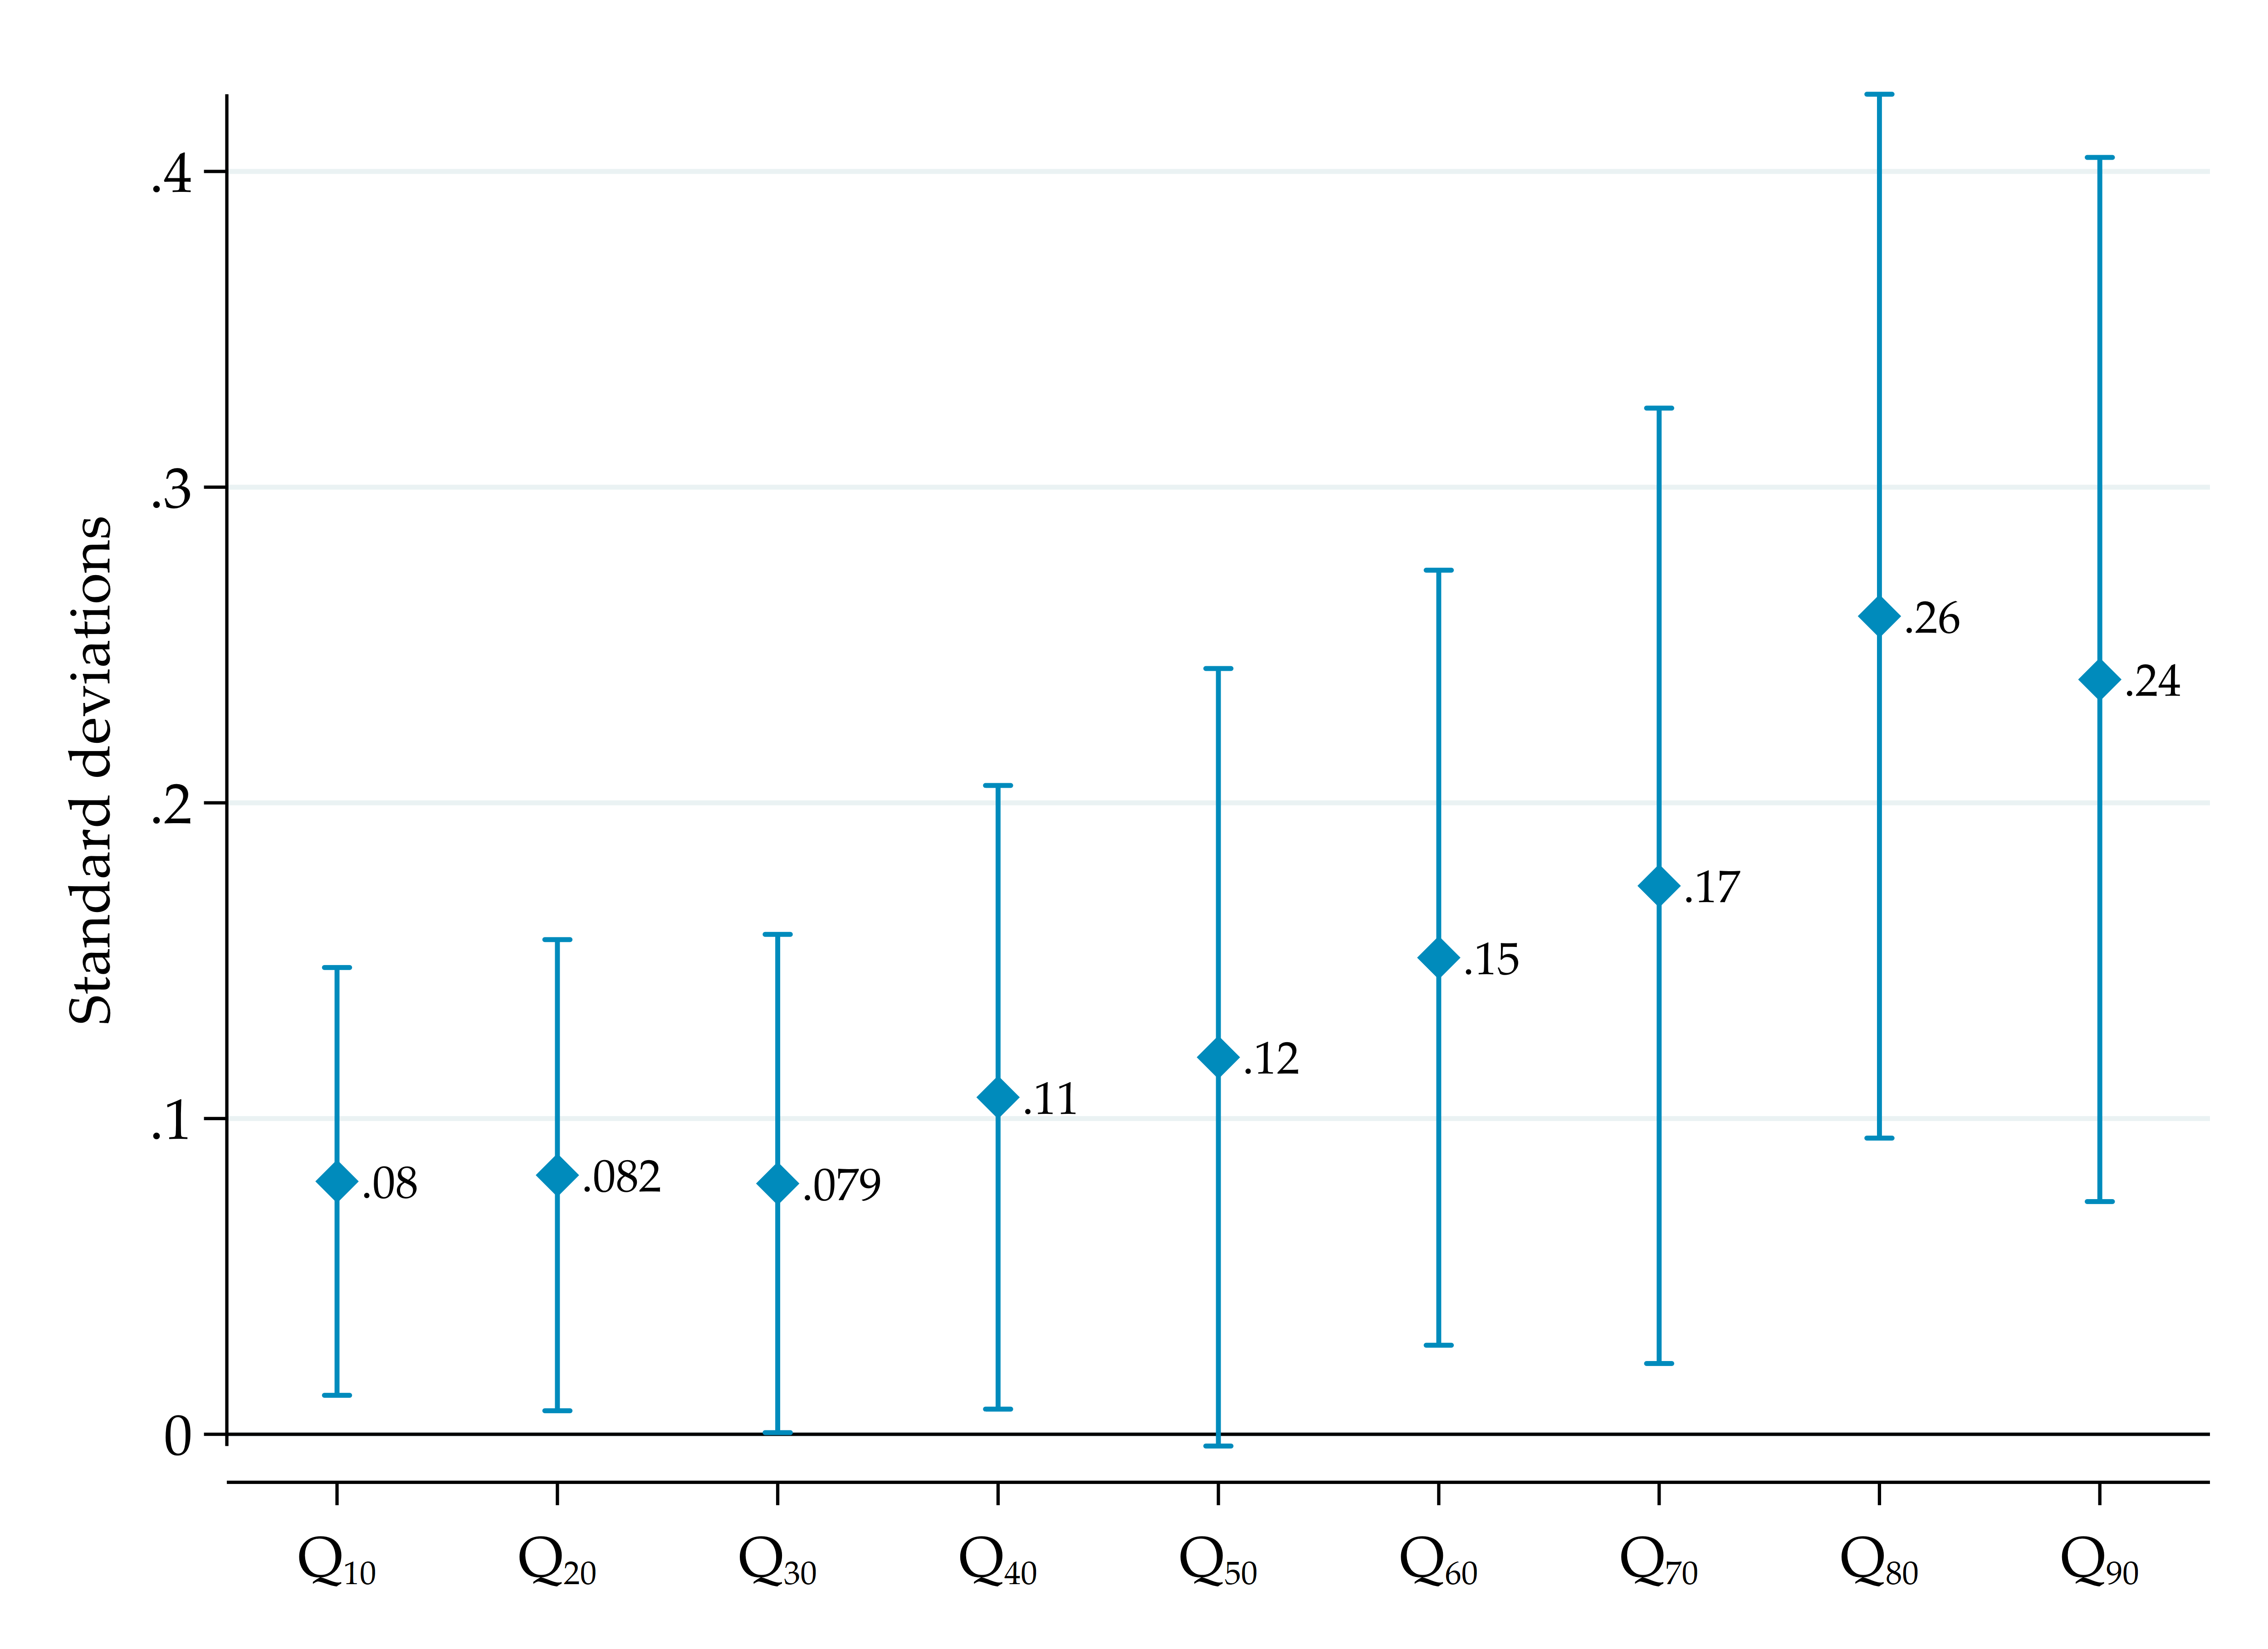
\includegraphics[width=14cm]{DataWork/Output/Figures/figA2-qreg_media_grade6.png}
		
		\begin{minipage}{0.825\textwidth}
			\small{\textit{Notes:} Point estimates of quantile regressions with strata (i.e., region) fixed effects and standard errors clustered at the school level. Confidence intervals are 90\%. Sample: schools treated at 6\textsuperscript{th} grade.}
		\end{minipage}
	\end{figure}
	
	\begin{figure}[ht!]
		\centering
		\caption{Impact on Average Test Score by Gender in 6\textsuperscript{th} Grade}
		\captionsetup[subfigure]{position=top,justification=centering}
		\label{fig:grade6_byGender}
		
		\begin{subfigure}{\textwidth}
			\caption{Distribution}
			\label{fig:kdensity_grade6_byGender}
			\centering
			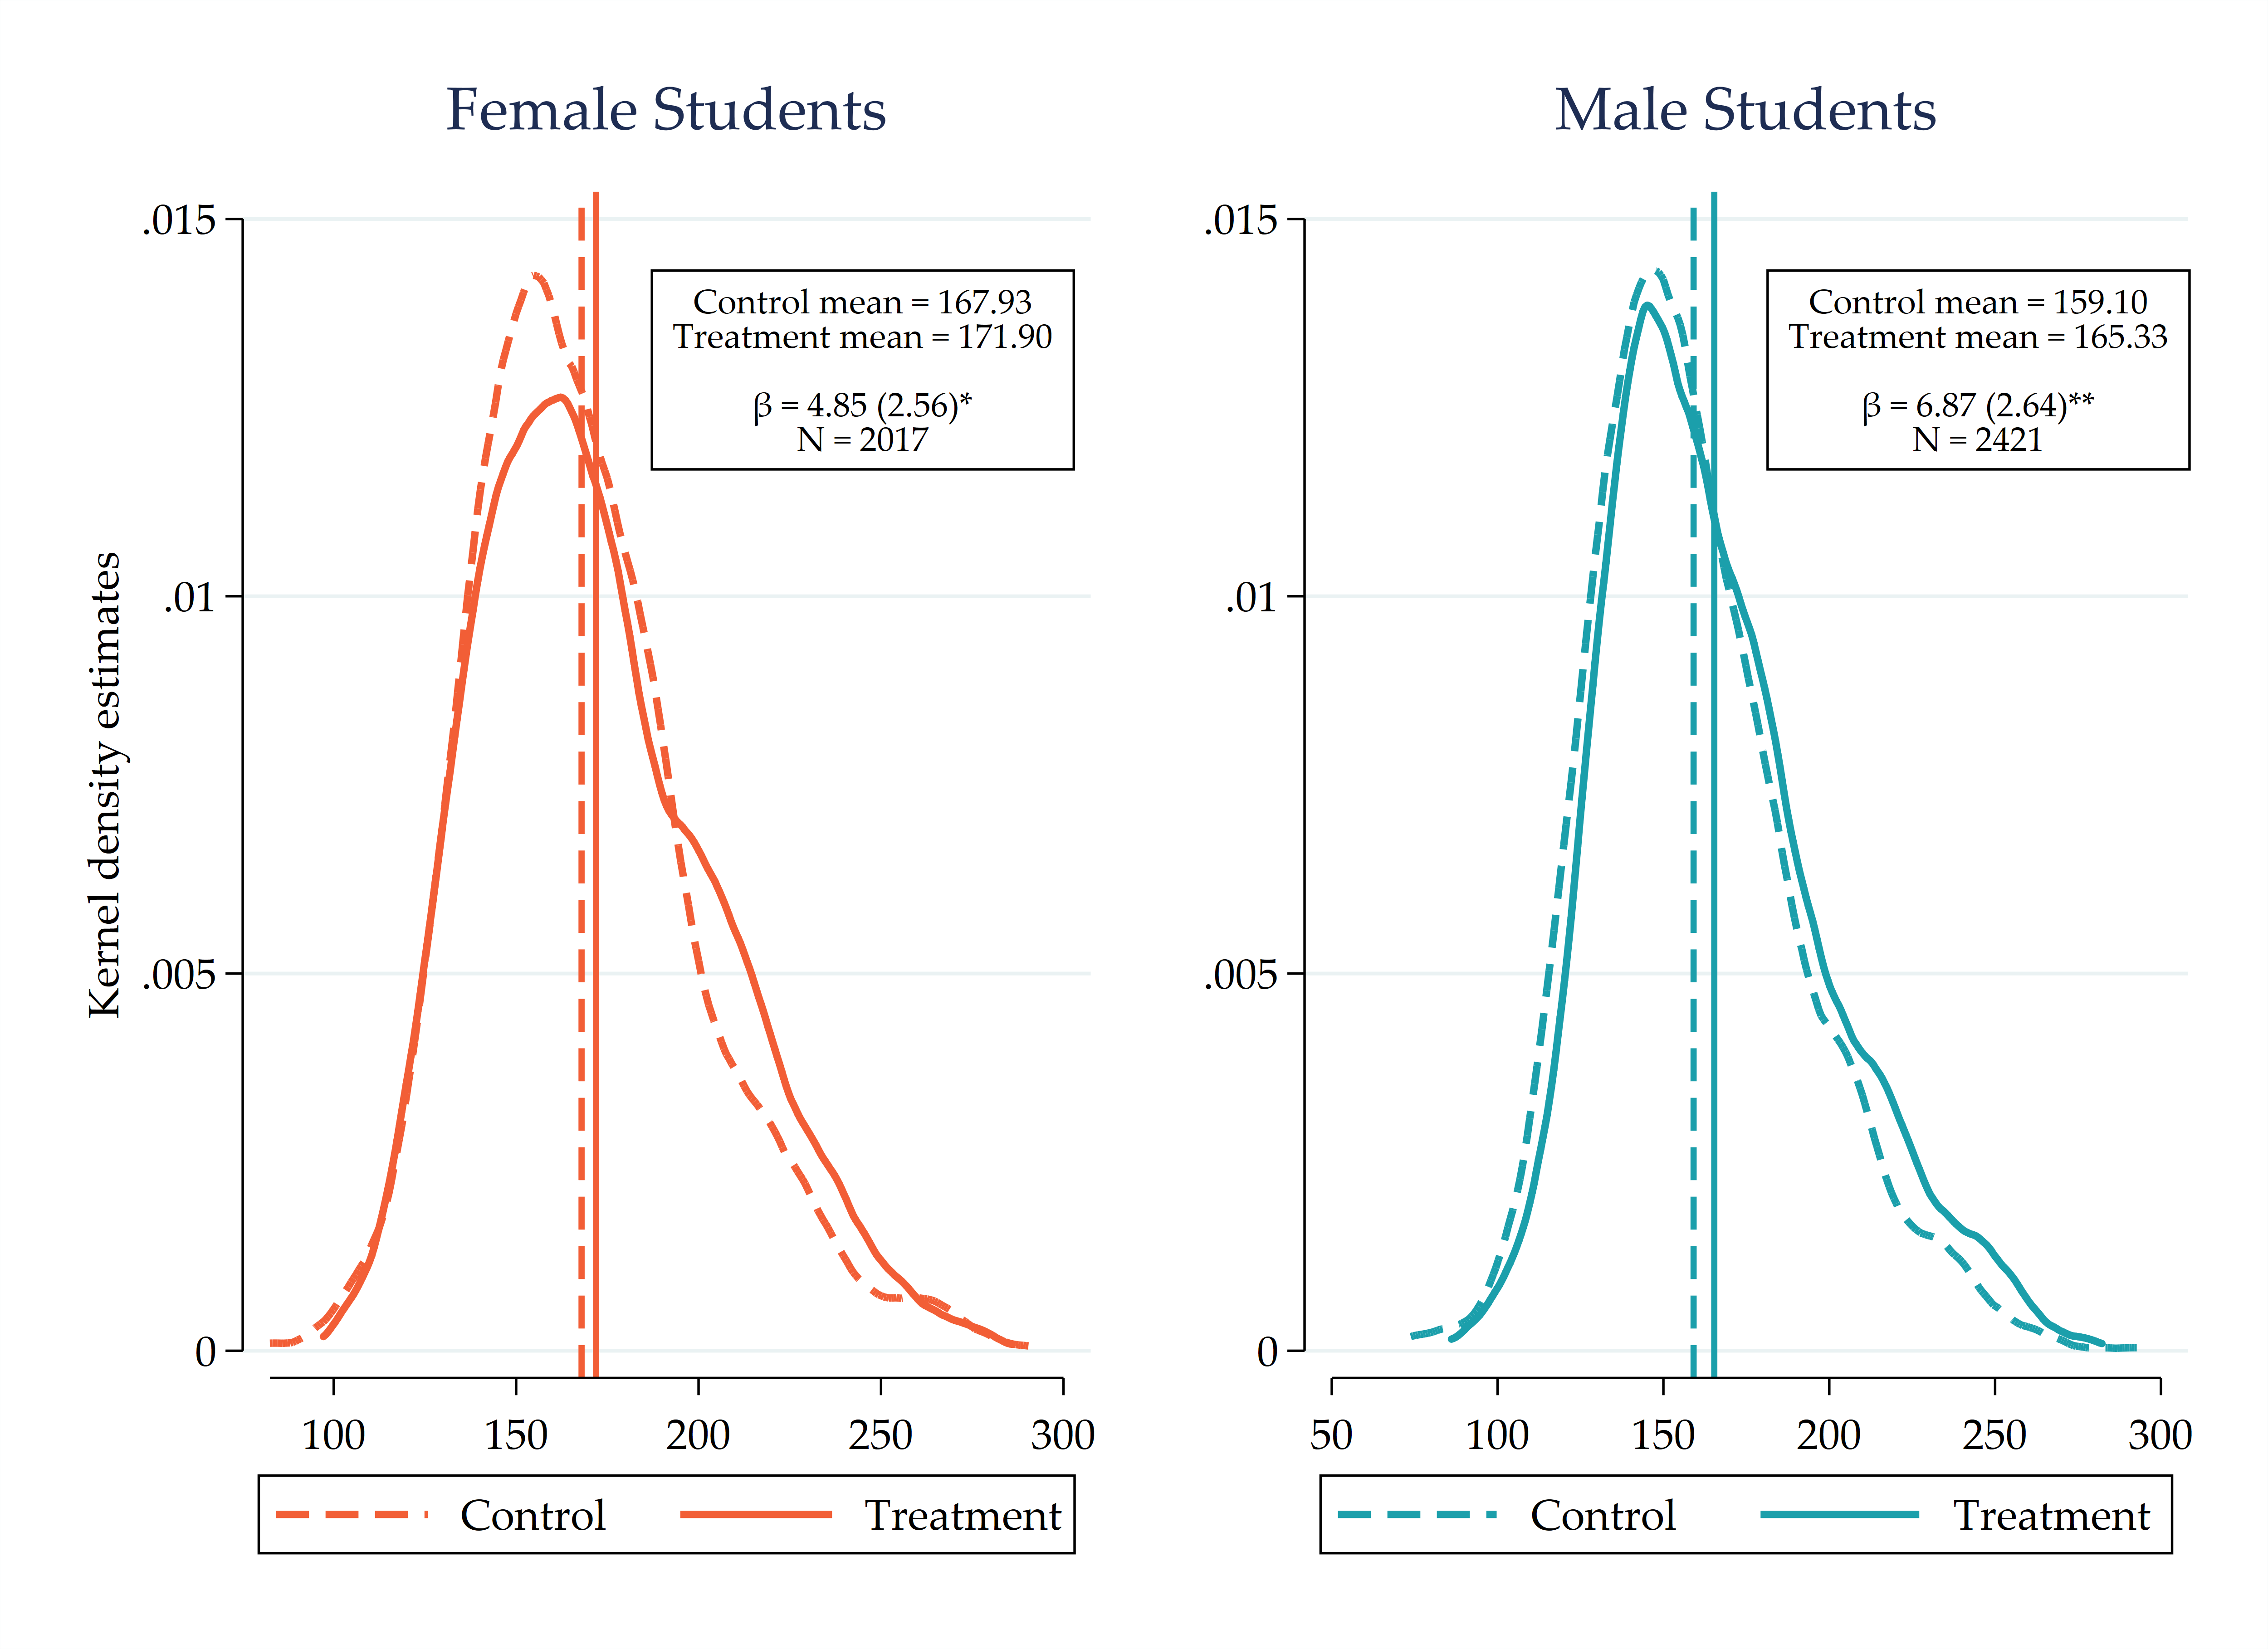
\includegraphics[width=14cm]{DataWork/Output/Figures/figA3a-kdensity_grade6_byGender.png}
		\end{subfigure}
		
		\begin{subfigure}{\textwidth}
			\caption{Quantile Treatment Effect}
			\label{fig:qreg_media_grade6_byGender}
			\centering
			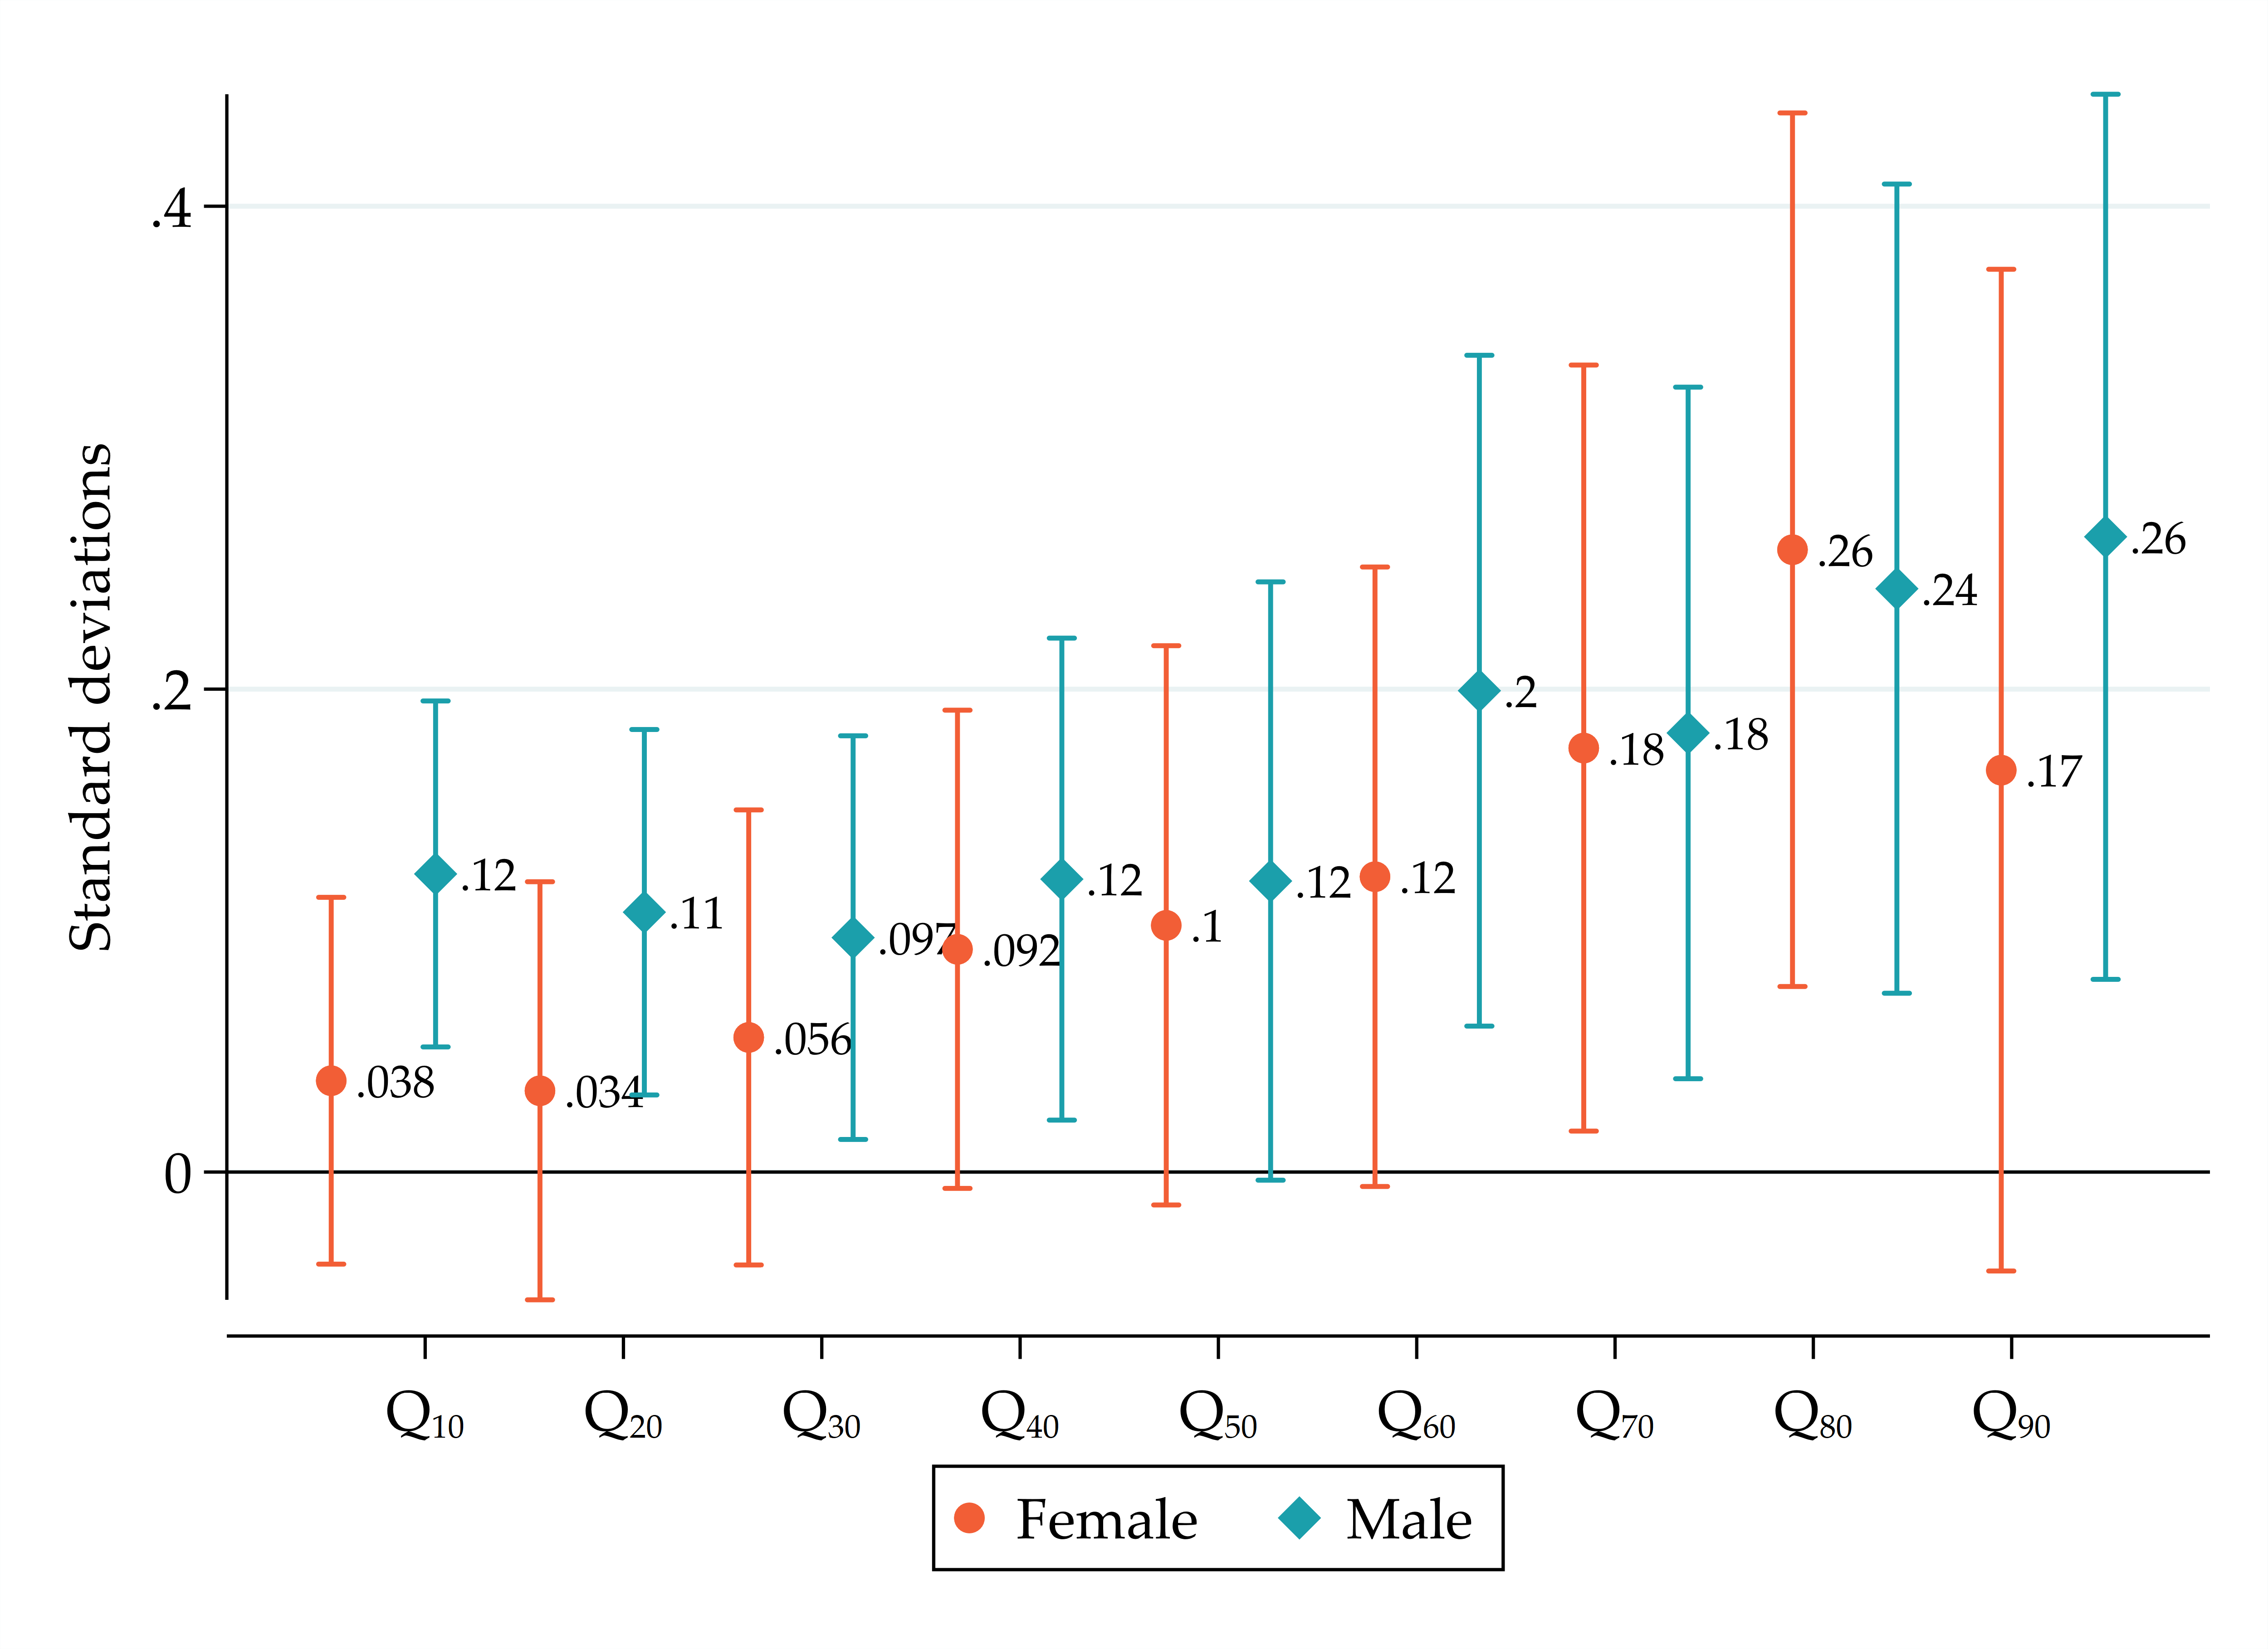
\includegraphics[width=14cm]{DataWork/Output/Figures/figA3b-qreg_media_grade6_byGender.png}
		\end{subfigure}
		
		\begin{minipage}{0.85\textwidth}
			\small{\textit{Notes:} Average test score is the average of standardized test scores in math, Portuguese, human and social science (range 0-400). Sample: schools treated at 6\textsuperscript{th} grade. Kernel densities are computed using Epanechnikov kernel function. Treatment effects in (a) are estimated through regressions with strata (i.e., region and grade) fixed effects and standard errors clustered at the school level. ** and * indicate significance at the 5 and 10 percent critical level. In (b), we plot point estimates of quantile regressions with 90\% confidence intervals. Quantile treatment effects are expressed in terms of standard deviations from the control group.}
		\end{minipage}
	\end{figure}
	
	% Figures for Policy Analysis
	\begin{figure}[ht!]
		\centering
		\caption{Learning Gains in 6\textsuperscript{th} Grade Rescaled to SAEB -- Projection over Time}
		\captionsetup[subfigure]{position=top,justification=centering}
		\label{fig:itt_ProvaBrasil}
		
		\begin{subfigure}{\textwidth}
			\centering
			\caption{Math}
			\label{fig:itt_ProvaBrasil_MT}
			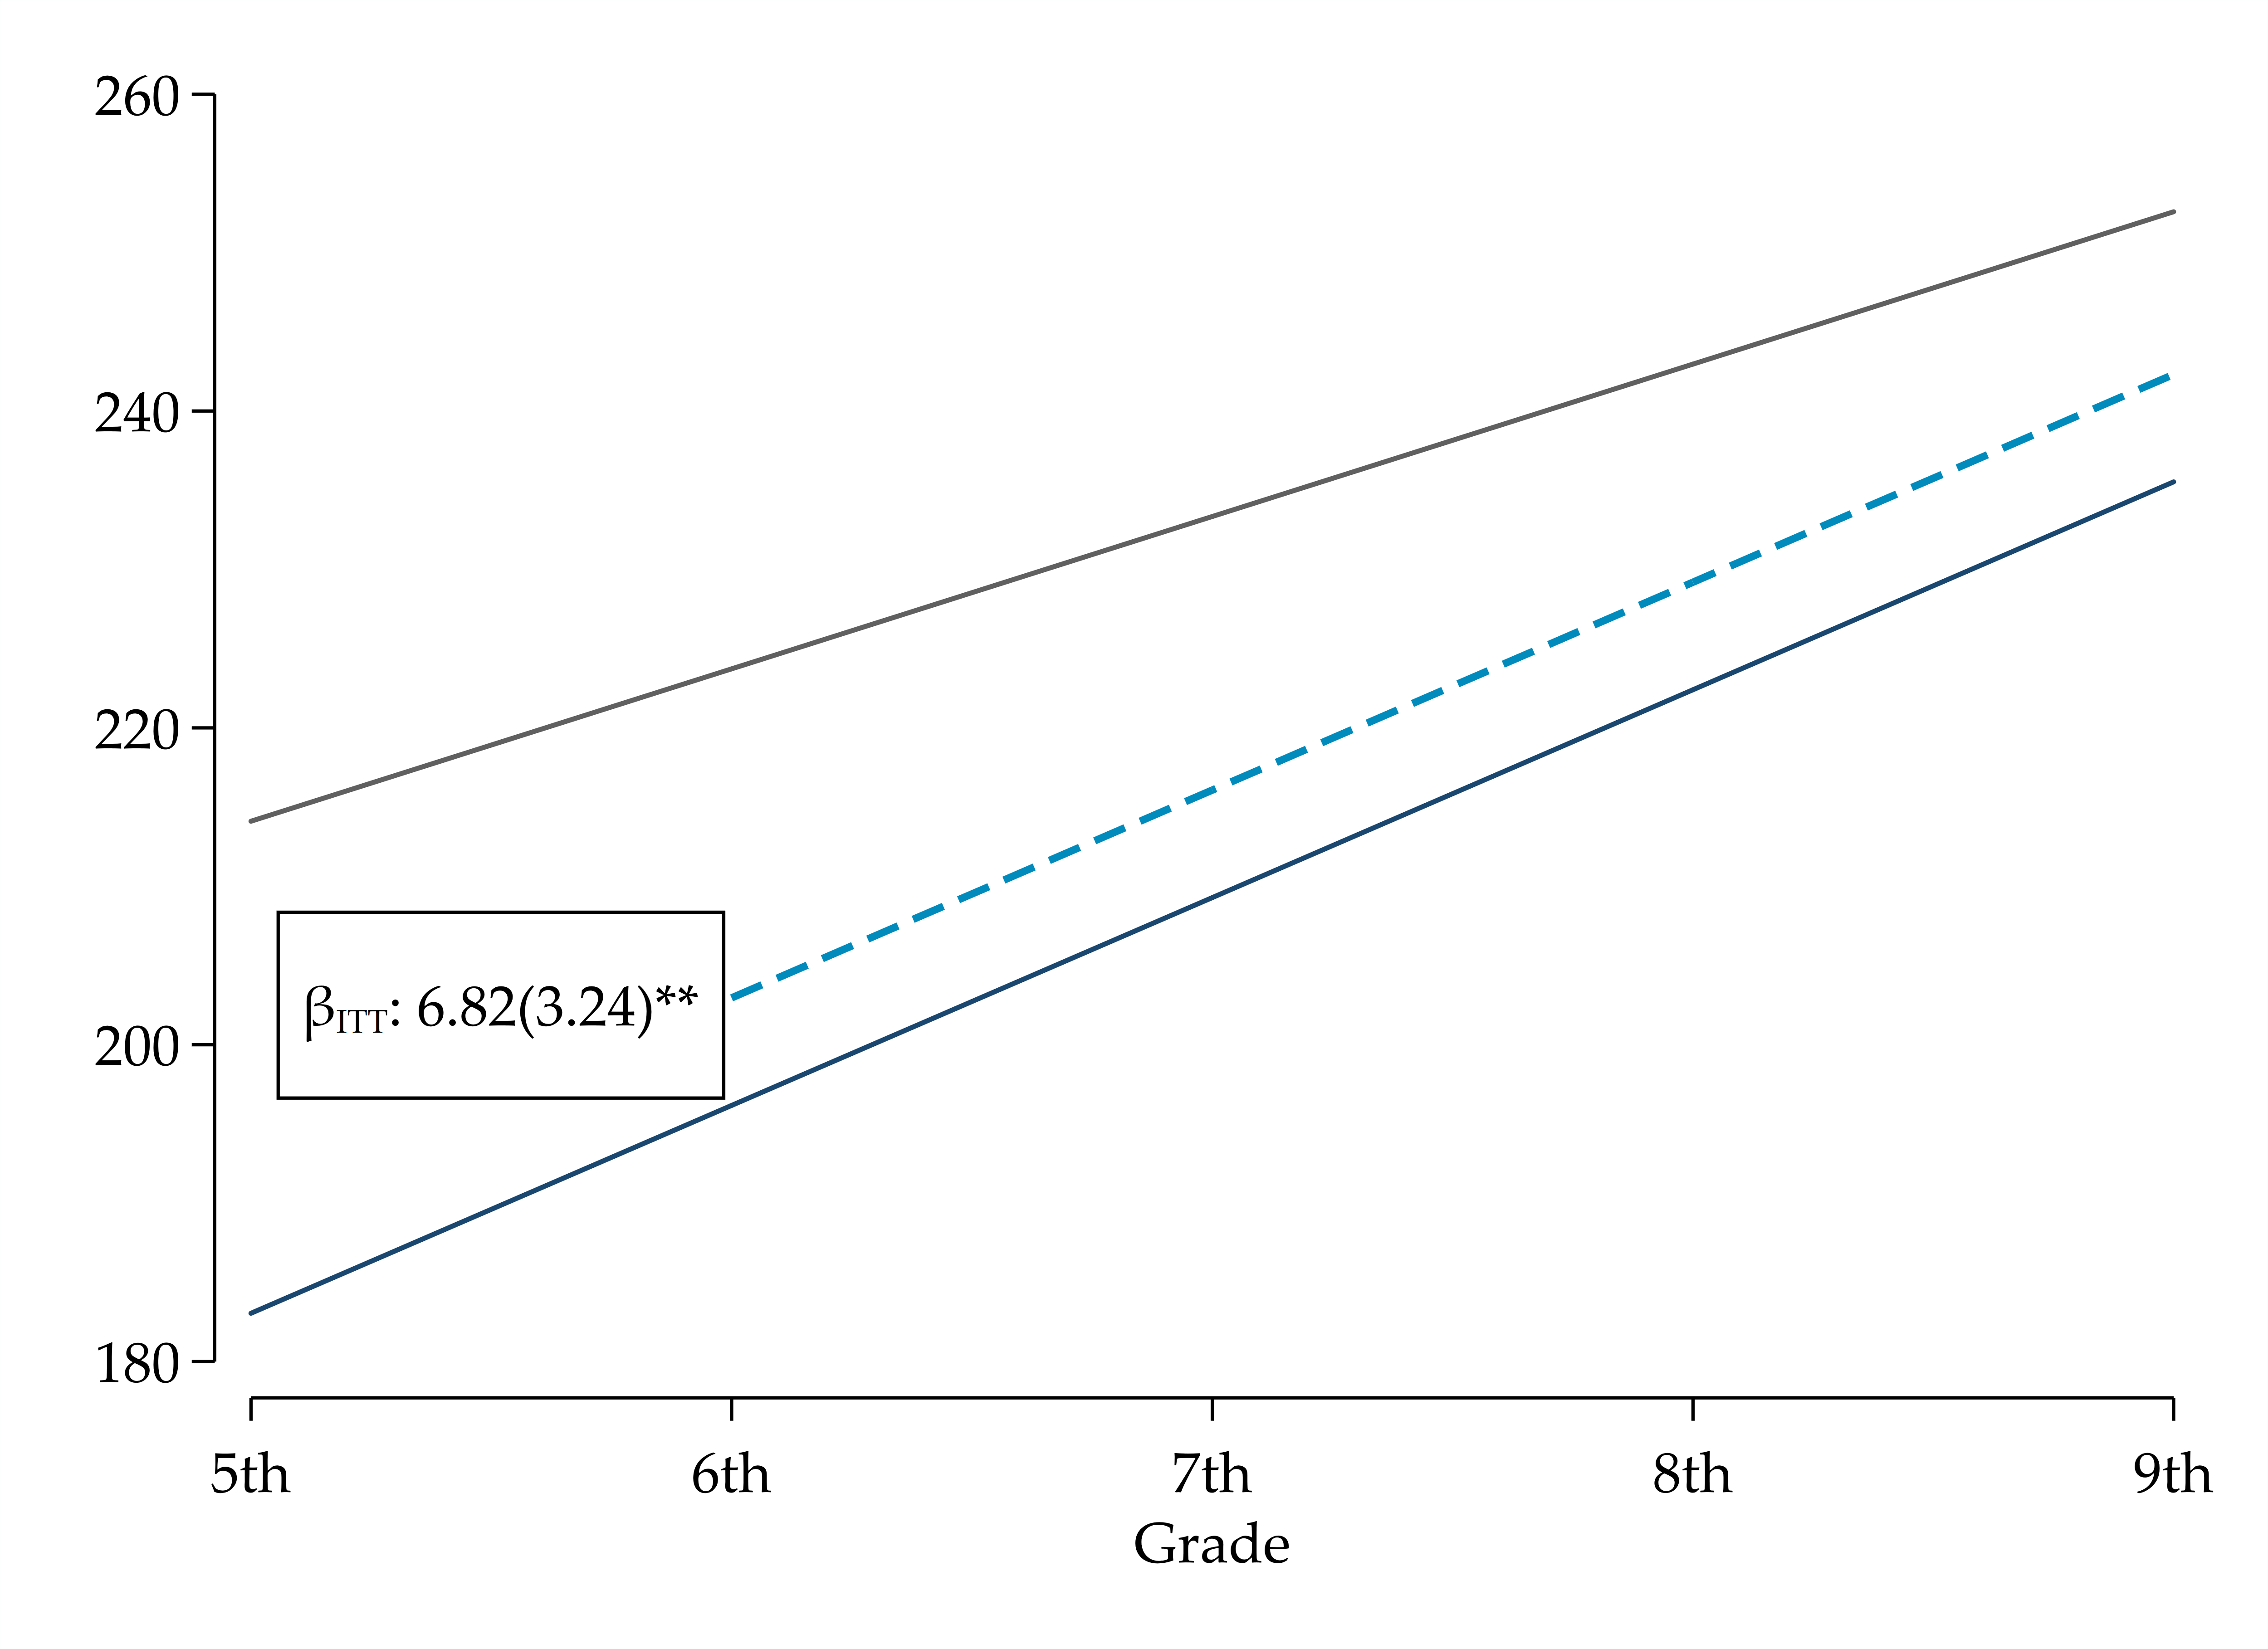
\includegraphics[width=13cm, height=8.75cm]{DataWork/Output/Figures/figA4a-itt_ProvaBrasil_MT.png}
		\end{subfigure}
		\begin{subfigure}{\textwidth}
			\centering
			\caption{Portuguese}
			\label{fig:itt_ProvaBrasil_PT}
			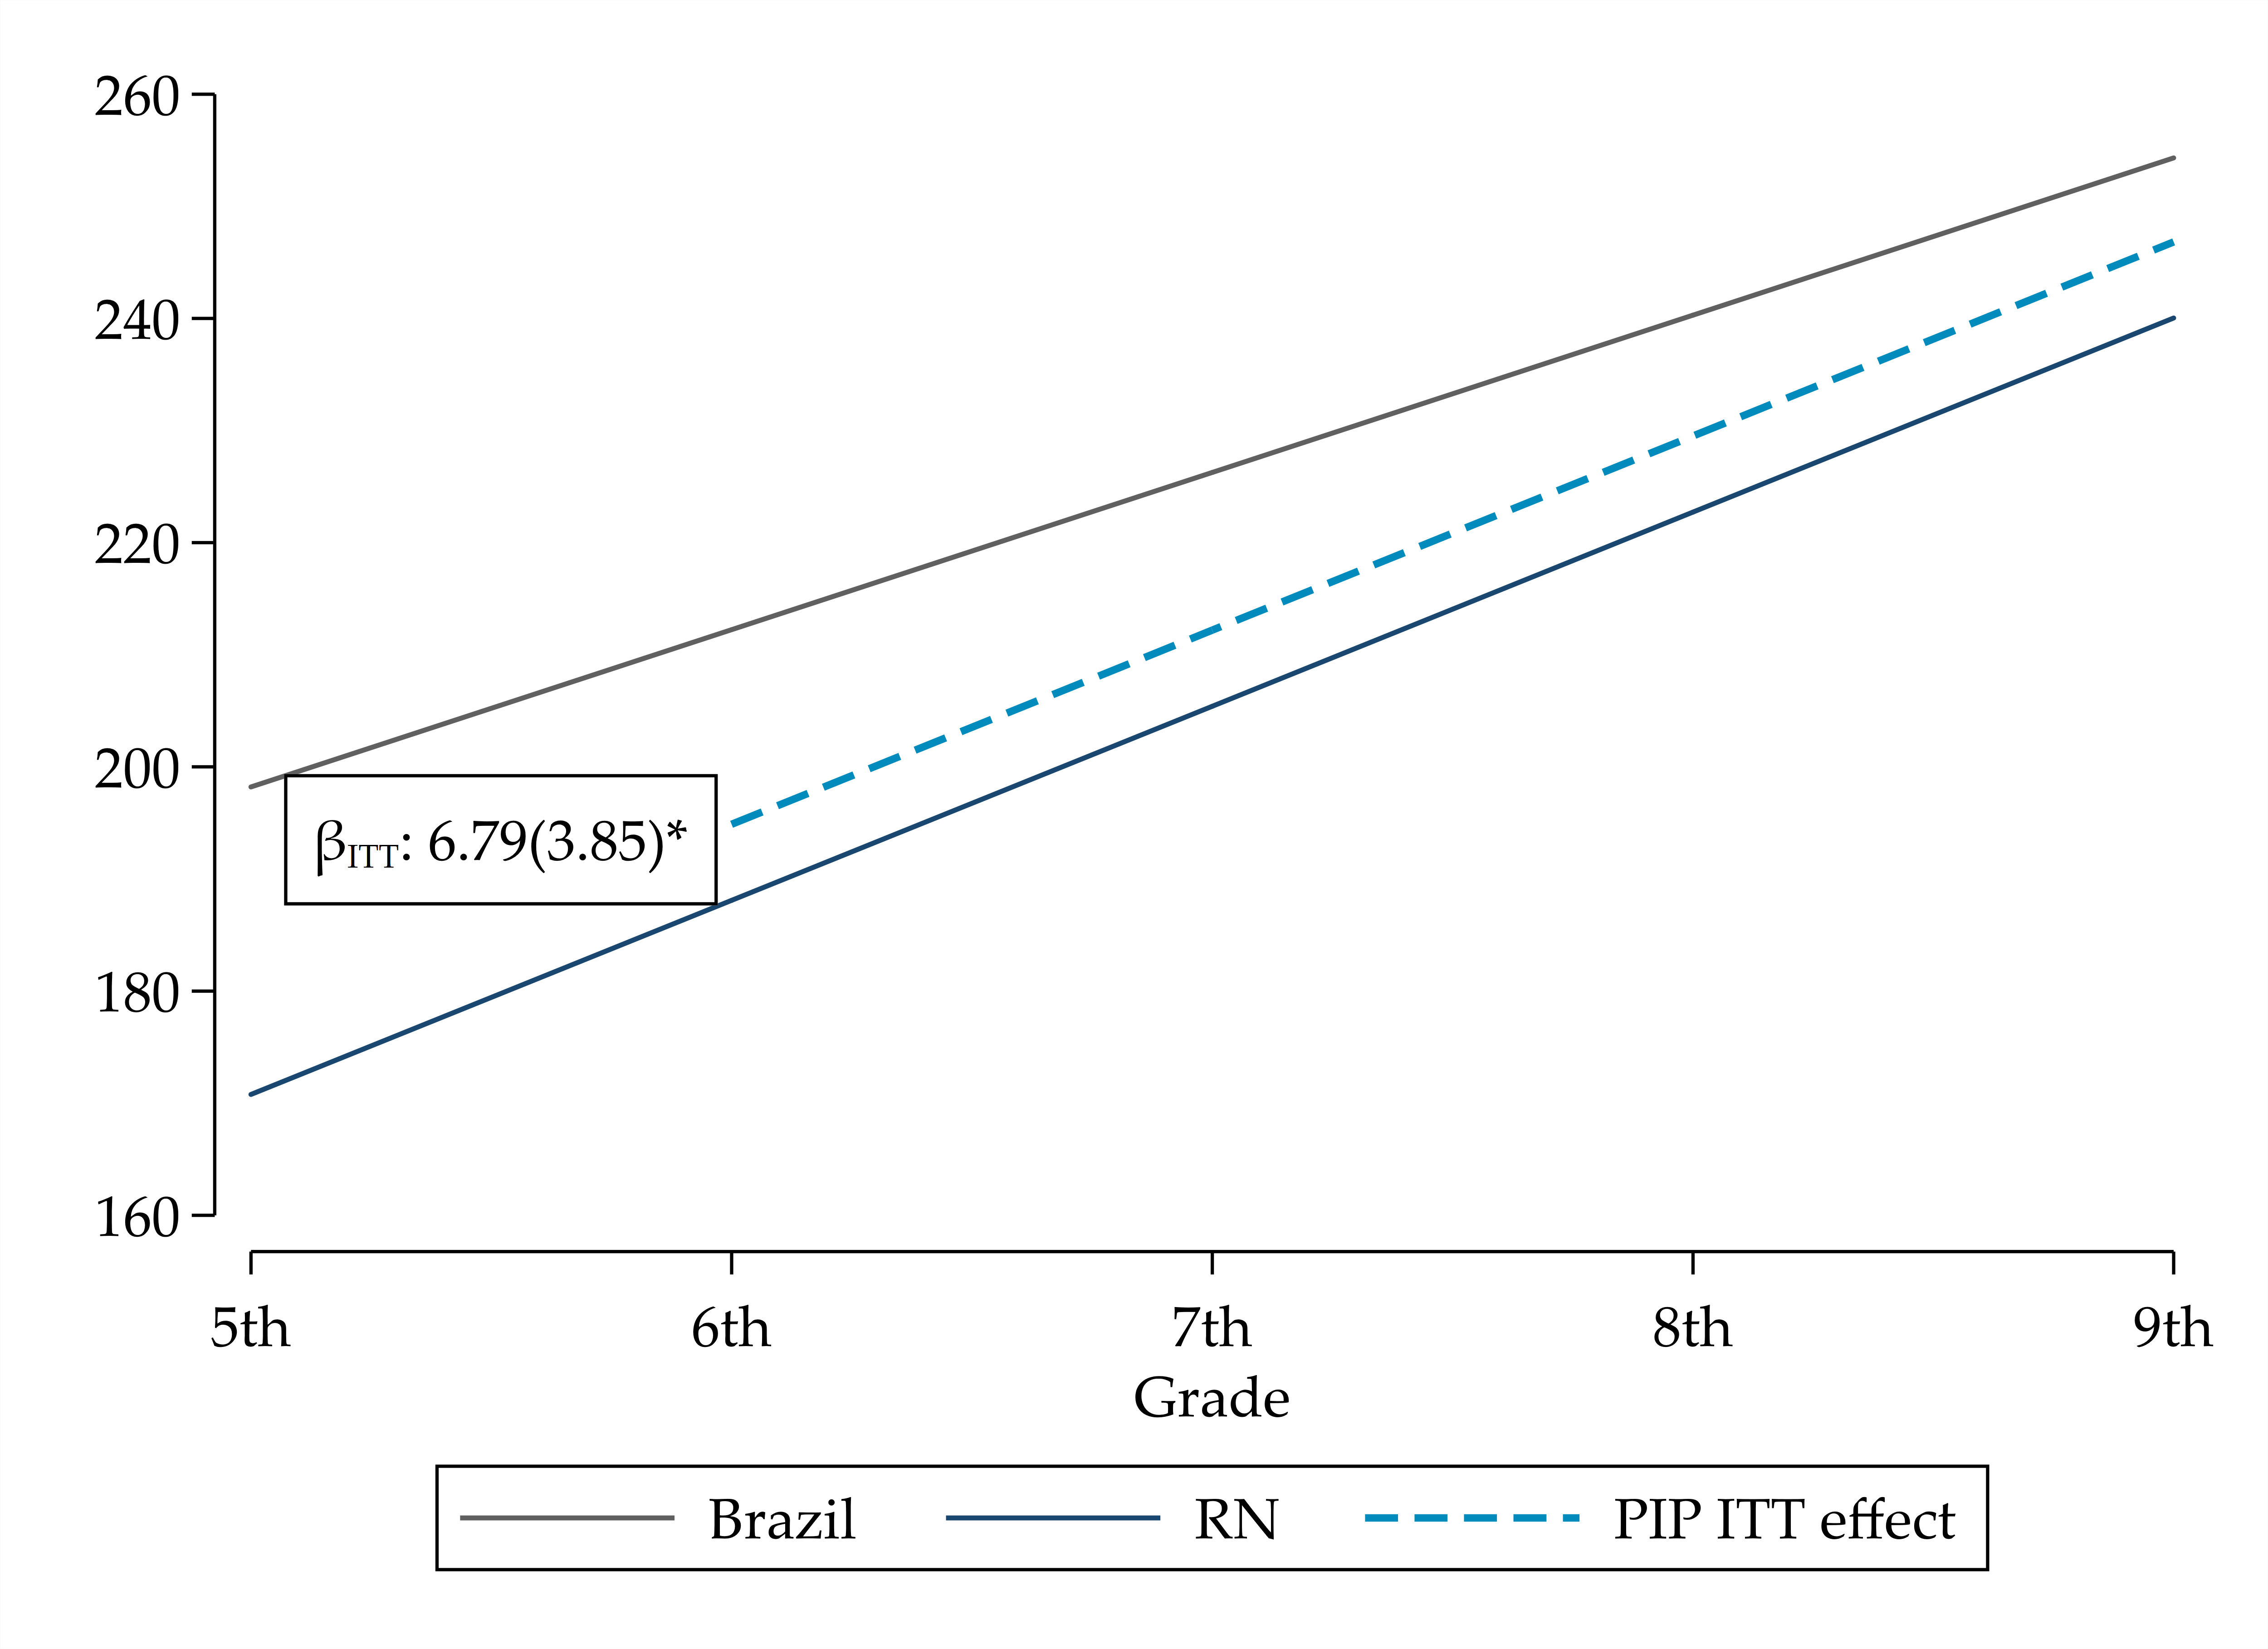
\includegraphics[width=13cm]{DataWork/Output/Figures/figA4b-itt_ProvaBrasil_LT.png}
		\end{subfigure}
		
		\begin{minipage}{0.825\textwidth}
			\small{\textit{Notes:} We use data from \textit{Instituto Nacional de Estudos e Pesquisas Educacionais Anísio Teixeira} (INEP) for state public schools in Rio Grande do Norte and Brazil. In particular, we use the average for the cohort who was in 5\textsuperscript{th} grade in 2013 and 9\textsuperscript{th} grade in 2017. The points in 6\textsuperscript{th}, 7\textsuperscript{th}, and 8\textsuperscript{th} grades are linear interpolation. The PIP intent-to-treat effect on 6\textsuperscript{th} graders is estimated through OLS with strata (i.e., region and grade) fixed effects and standard errors clustered at the school level. **, and * indicate significance at the 5, and 10 percent critical level.}
		\end{minipage}
		
	\end{figure}
	
	\vfill
	\begin{figure}[ht!]
		\centering
		\caption{Learning Gains in 6\textsuperscript{th} Grade Rescaled to \textit{IDEB} -- Comparison with Other Brazilian States}
		
		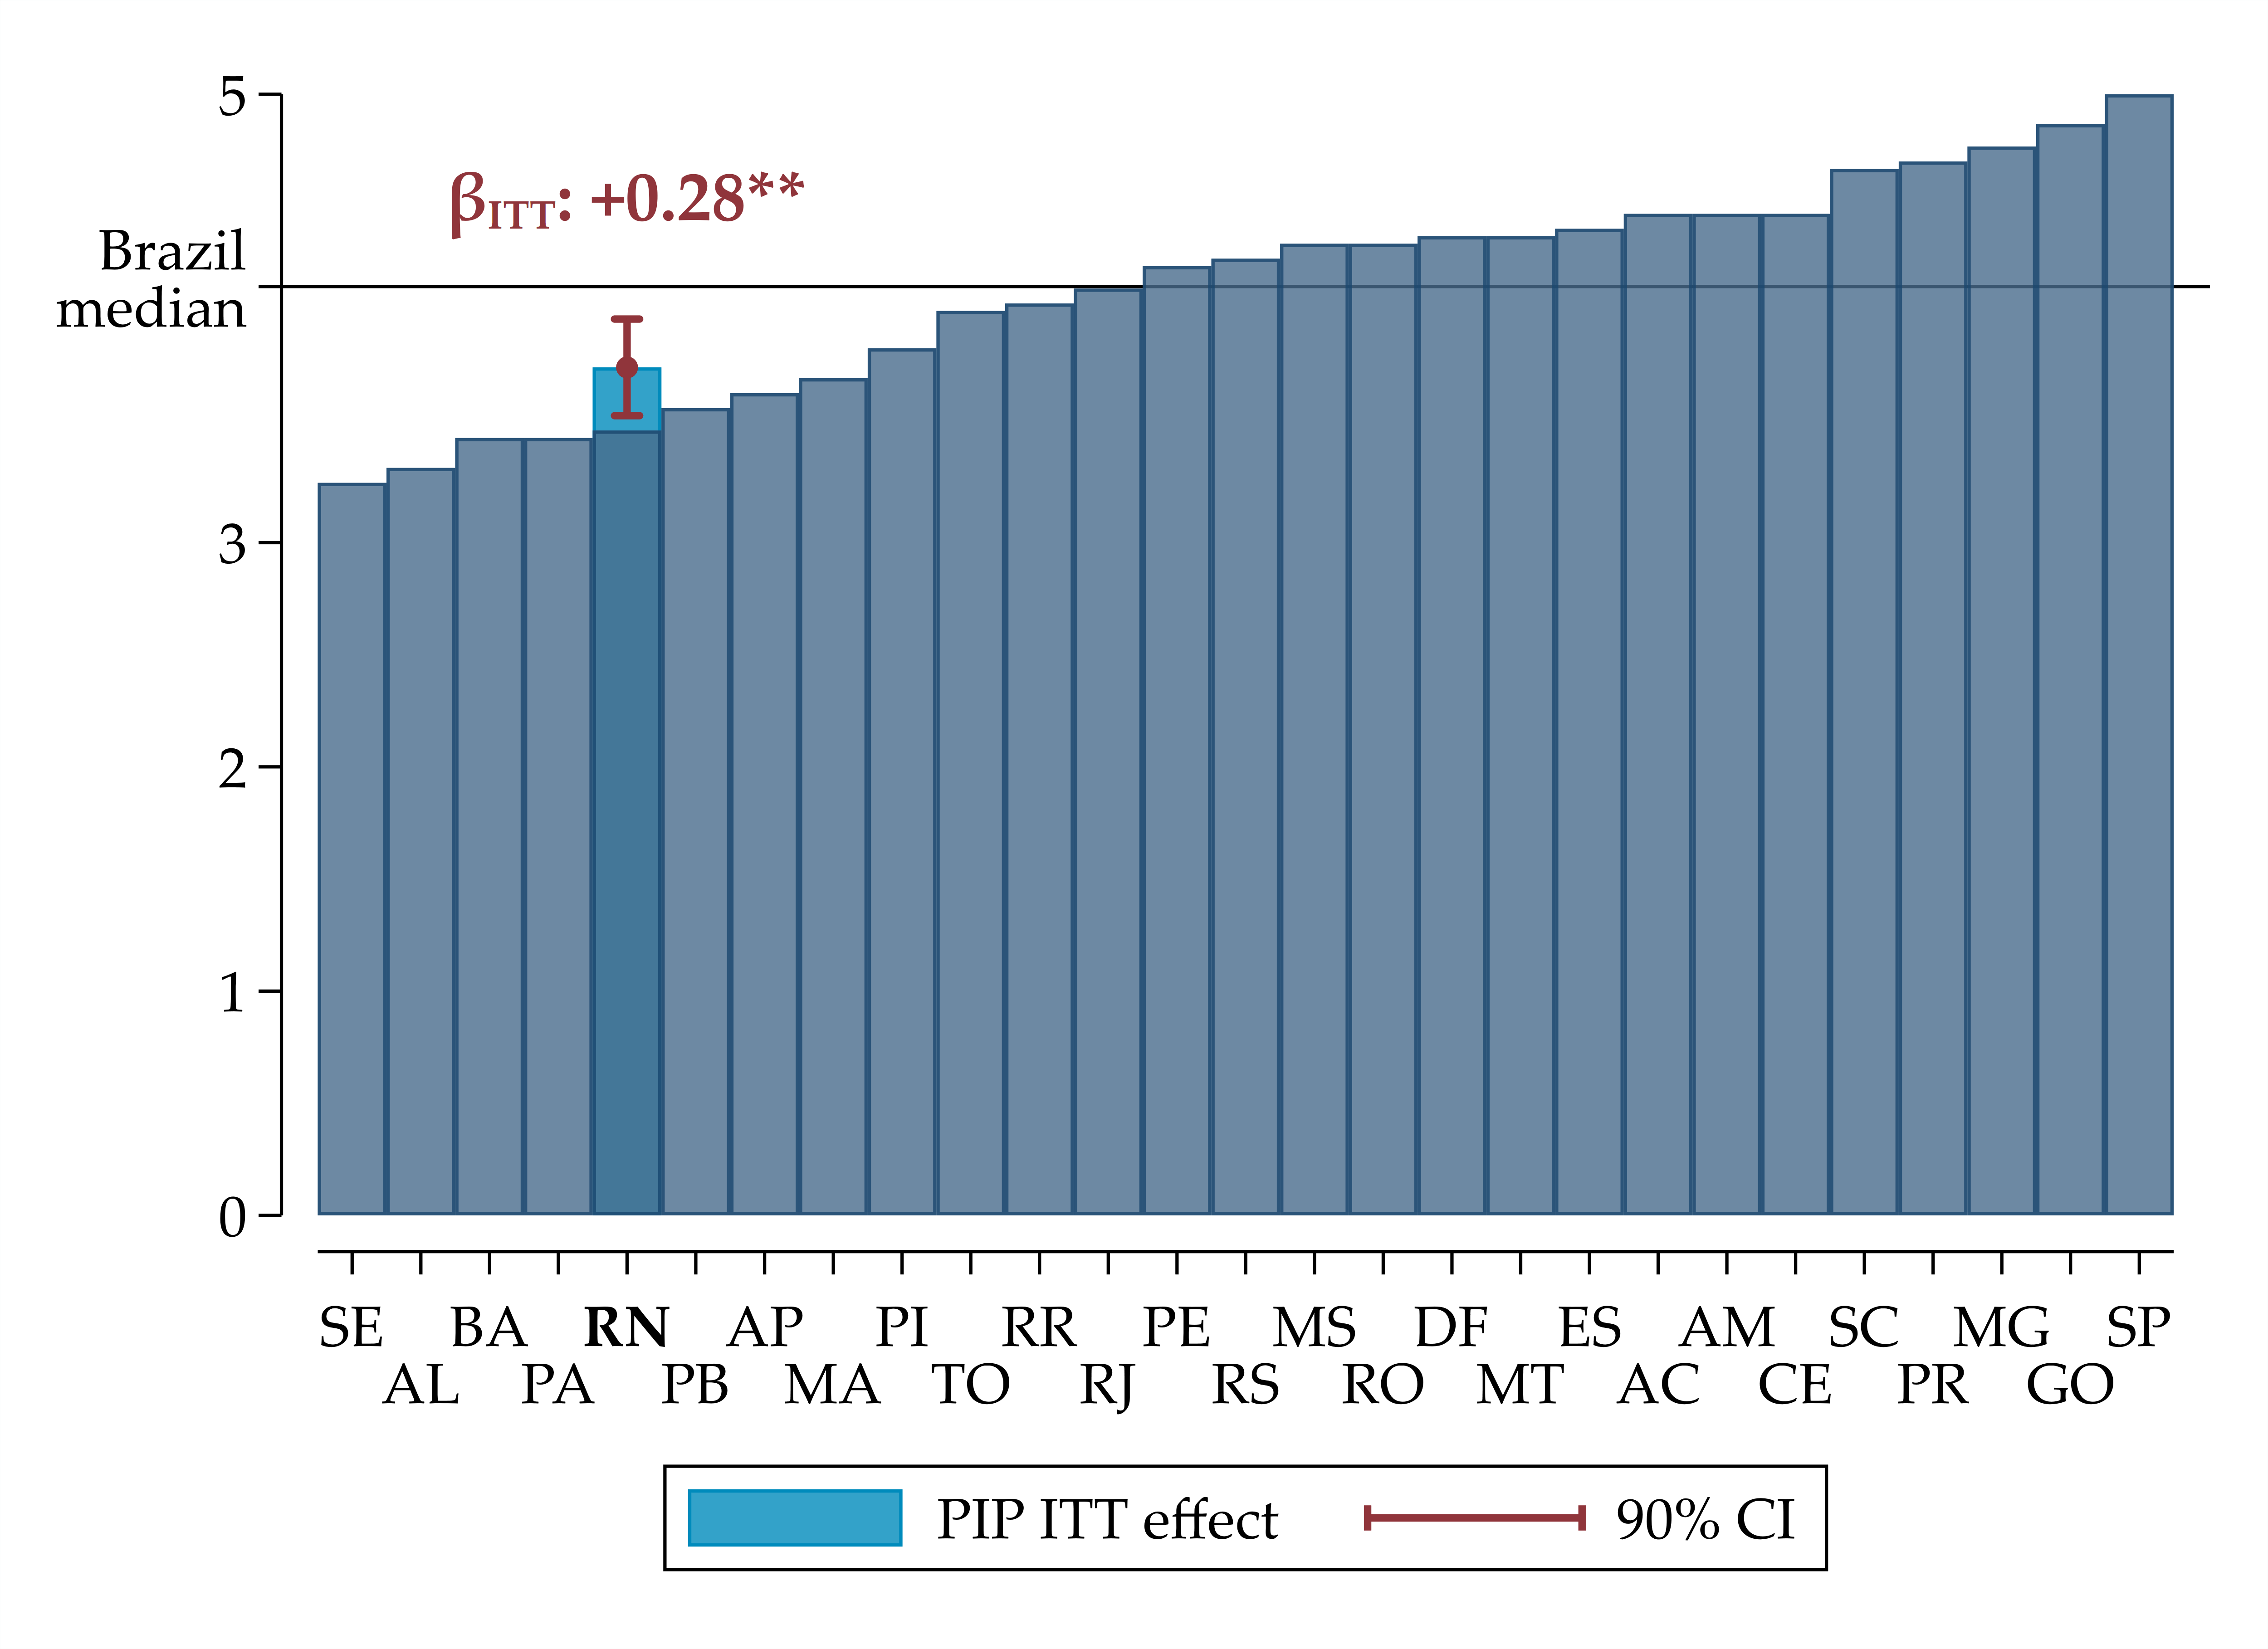
\includegraphics[width=14cm]{DataWork/Output/Figures/figA5-itt_IDEB.png}
		\label{fig:itt_IDEB}
		
		\begin{minipage}{0.825\textwidth}
			\small{\textit{Notes:} We use data from \textit{Instituto Nacional de Estudos e Pesquisas Educacionais Anísio Teixeira} (INEP) for state public schools. The bars show average IDEB by state in 2015. The PIP intent-to-treat effect on 6\textsuperscript{th} graders is estimated through OLS with strata (i.e., region and grade) fixed effects and robust standard errors. ** indicate significance at the 5 percent critical level. See \ref{sec:ideb} for the methodology we follow to compute IDEB for our grades of interest.}
		\end{minipage}
		
	\end{figure}
	\vfill
	
	\clearpage
	
	% Balance in participation in tests
	\begin{table}[ht!]
		\caption{Balance in Socio-Emotional and Proficiency Test Participation}
		\label{tab:baltab_participation}
		\centering
		\begin{adjustbox}{totalheight=\textheight} 
			\begin{tabular}{lcccccccc} \hline \hline
				
                                        & (1) & (2)     & (3) & (4)     & (5) & (6)       & (7)     & (8)         \\[1.5ex]            
\textit{Variable}   &     & Total   &     & Control &     & Treatment & T-test  & RI      \\                           
\hspace{1em} Sample &  N  & Mean/SE &  N  & Mean/SE &  N  & Mean/SE   & P-value & P-value \\[1.5ex] \hline 
\addlinespace[0.5ex] \multicolumn{9}{c}{\textbf{Panel A -- Socio-emotional tests}}        \\[0.5ex] \hline 
                                 \addlinespace[0.5em] \textit{Participating schools}         \\[1em] \hspace{1em} All schools & 280 & 0.839 & 154 & 0.779 & 126 & 0.913 & 0.002 & 0.003 \\    &  & (0.022) &  & (0.034) &  & (0.025) &  &  \\  \hspace{1em} 5th grade & 97 & 0.876 & 52 & 0.827 & 45 & 0.933 & 0.125 & 0.151 \\   &  & (0.034) &  & (0.053) &  & (0.038) &  &  \\  \hspace{1em} 6th grade & 105 & 0.829 & 59 & 0.780 & 46 & 0.891 & 0.124 & 0.149 \\   &  & (0.037) &  & (0.054) &  & (0.046) &  &  \\  \hspace{1em} 10th grade & 78 & 0.808 & 43 & 0.721 & 35 & 0.914 & 0.025 & 0.038 \\   &  & (0.045) &  & (0.069) &  & (0.048) &  &  \\  \textit{Percentage of test takers} \\[1em] \hspace{1em} All schools & 235 & 0.549 & 120 & 0.530 & 115 & 0.570 & 0.180 & 0.184 \\   &  & (0.015) &  & (0.021) &  & (0.021) &  &  \\  \hspace{1em} 5th grade & 85 & 0.578 & 43 & 0.547 & 42 & 0.610 & 0.209 & 0.210 \\   &  & (0.024) &  & (0.030) &  & (0.036) &  &  \\  \hspace{1em} 6th grade & 87 & 0.545 & 46 & 0.539 & 41 & 0.551 & 0.823 & 0.826 \\   &  & (0.024) &  & (0.034) &  & (0.033) &  &  \\  \hspace{1em} 10th grade & 63 & 0.517 & 31 & 0.492 & 32 & 0.541 & 0.392 & 0.412 \\   &  & (0.031) &  & (0.048) &  & (0.042) &  &  \\                                                                                                                                                                   [1.8ex] \hline 
\addlinespace[0.5ex] \multicolumn{9}{c}{\textbf{Panel B -- Proficiency tests}}                    \\[0.5ex] \hline 
                                 \addlinespace[0.5em] \textit{Participating schools}     \\[1em] \hspace{1em} All schools & 280 & 0.943 & 154 & 0.942 & 126 & 0.944 & 0.941 & 1.000 \\    &  & (0.014) &  & (0.019) &  & (0.020) &  &  \\  \hspace{1em} 5th grade & 97 & 0.948 & 52 & 0.942 & 45 & 0.956 & 0.888 & 0.906 \\   &  & (0.023) &  & (0.033) &  & (0.031) &  &  \\  \hspace{1em} 6th grade & 105 & 0.943 & 59 & 0.949 & 46 & 0.935 & 0.698 & 0.688 \\   &  & (0.023) &  & (0.029) &  & (0.037) &  &  \\  \hspace{1em} 10th grade & 78 & 0.936 & 43 & 0.930 & 35 & 0.943 & 0.289 & 0.467 \\   &  & (0.028) &  & (0.039) &  & (0.040) &  &  \\  \textit{Percentage of test takers} \\[1em] \hspace{1em} All schools & 264 & 0.696 & 145 & 0.699 & 119 & 0.691 & 0.775 & 0.778 \\   &  & (0.015) &  & (0.019) &  & (0.023) &  &  \\  \hspace{1em} 5th grade & 92 & 0.408 & 49 & 0.418 & 43 & 0.396 & 0.256 & 0.264 \\   &  & (0.008) &  & (0.009) &  & (0.013) &  &  \\  \hspace{1em} 6th grade & 99 & 0.853 & 56 & 0.840 & 43 & 0.870 & 0.245 & 0.264 \\   &  & (0.013) &  & (0.018) &  & (0.019) &  &  \\  \hspace{1em} 10th grade & 73 & 0.845 & 40 & 0.848 & 33 & 0.841 & 0.720 & 0.723 \\   &  & (0.016) &  & (0.022) &  & (0.025) &  &  \\                                                                                                                                              [1.8ex]  \hline \hline \\[-1.5ex]


				\multicolumn{9}{@{}p{1.06\textwidth}}{\textit{Notes}: `\textit{Participating schools}' is a dummy for schools which had at least one test taker. `\textit{Percentage of test takers}' is defined as the percentage of students who took the test for each school in the sample, conditional on the school being a `participating school'. Robust standard errors (SE) in parentheses. Strata (i.e., region) fixed effects are included in all the estimated regressions. We show both standard p-values and p-values computed using randomization inference (RI) with 10,000 repetitions for the whole sample and each grade.} 
			\end{tabular}
		\end{adjustbox}
	\end{table}
	
	\begin{table}[ht!]
		\caption{Balance Table on Subsample of Schools with Socio-Emotional Test Takers}
		\label{tab:baltab_socio_schoollevel}
		\centering
		\begin{adjustbox}{max width=\textwidth}
			\begin{tabular}{lcccccccc} \hline \hline
				                  & \multicolumn{5}{c}{\textbf{All schools}}                                      & 5th Grade    & 6th Grade    & 10th Grade   \\                       
                        \cmidrule(lr){2-6} \cmidrule(lr){7-7} \cmidrule(lr){8-8} \cmidrule(lr){9-9}                                                                    \\[-2ex]              
                  & (1)                  & (2)         & (3)                   & (4)           & (5)          & (6)              & (7)          & (8)                  \\                               
                  &                      &             &                               &                       & T-test       & T-test           & T-test       & T-test               \\                               
                  &                      & Control &                           & Treatment & P-value      & P-value      & P-value      & P-value              \\                               
 Variable & N/[Clusters] & Mean/SE &  N/[Clusters] & Mean/SE   & [RI p-value] & [RI p-value] & [RI p-value] & [RI p-value] \\ \hline \\[-2ex]
\multicolumn{9}{c}{\textbf{Panel A -- School characteristics}}                                                                                                                         \\[0.5ex] \hline 
                                   \addlinespace[0.75ex] Has access to internet & 120 & 0.917 & 115 & 0.957 & 0.227 & 0.182 & 0.501 & 0.947 \\    &  & (0.025) &  & (0.019) & [0.288] & [0.373] & [0.680] & [1.000] \\  Has library & 120 & 0.642 & 115 & 0.661 & 0.839 & 0.853 & 0.602 & 0.179 \\   &  & (0.044) &  & (0.044) & [0.879] & [1.000] & [0.662] & [0.359] \\  Has sciences lab & 120 & 0.125 & 115 & 0.174 & 0.243 & N/A & 0.636 & 0.137 \\   &  & (0.030) &  & (0.035) & [0.254] & [1.000] & [1.000] & [0.203] \\  Located in urban area & 120 & 1.175 & 115 & 1.113 & 0.179 & 0.173 & 0.747 & 0.438 \\   &  & (0.035) &  & (0.030) & [0.249] & [0.267] & [0.783] & [0.500] \\  Distance to Natal (km) & 117 & 143.815 & 114 & 148.243 & 0.739 & 0.895 & 0.681 & 0.732 \\   &  & (10.416) &  & (10.806) & [0.742] & [0.896] & [0.678] & [0.736] \\  Number of employees & 120 & 30.100 & 115 & 28.904 & 0.365 & 0.609 & 0.502 & 0.691 \\   &  & (1.269) &  & (1.161) & [0.366] & [0.617] & [0.499] & [0.688] \\  Number of students & 120 & 379.800 & 115 & 360.304 & 0.419 & 0.956 & 0.607 & 0.449 \\   &  & (22.390) &  & (24.342) & [0.430] & [0.957] & [0.602] & [0.462] \\  Number of classes & 120 & 15.425 & 115 & 14.096 & 0.160 & 0.600 & 0.234 & 0.426 \\   &  & (0.787) &  & (0.815) & [0.164] & [0.605] & [0.230] & [0.442] \\  Students per class & 120 & 24.107 & 115 & 24.721 & 0.352 & 0.325 & 0.275 & 0.587 \\   &  & (0.572) &  & (0.540) & [0.352] & [0.326] & [0.268] & [0.581] \\ \hline \\[-2ex]                                                                                                                                                                                                                          
\multicolumn{9}{c}{\textbf{Panel B -- Grades assigned to the intervention}}                                                                                            \\[0.5ex] \hline 
                       \addlinespace[0.75ex] Passing rate & 120 & 71.697 & 114 & 73.711 & 0.333 & 0.511 & 0.277 & 0.885 \\    &  & (1.630) &  & (1.600) & [0.327] & [0.513] & [0.267] & [0.885] \\  Drop-out rate & 120 & 7.428 & 114 & 8.026 & 0.715 & 0.355 & 0.869 & 0.332 \\   &  & (0.848) &  & (0.953) & [0.717] & [0.360] & [0.869] & [0.324] \\  Retention rate & 120 & 20.876 & 114 & 18.263 & 0.195 & 0.668 & 0.249 & 0.567 \\   &  & (1.371) &  & (1.316) & [0.186] & [0.671] & [0.248] & [0.559] \\ \hline \\[-2ex]                                                                                                                                                                                                              
\multicolumn{9}{c}{\textbf{Panel C -- Teacher characteristics}}                                                                                                                        \\[0.5ex] \hline 
                           \addlinespace[0.75ex] Age & 783 & 40.553 & 780 & 40.010 & 0.343 & 0.342 & 0.920 & 0.320 \\    & [119] & (0.381) & [115] & (0.392) & [0.364] & [0.340] & [0.920] & [0.337] \\  Gender (male $= 1$) & 783 & 0.466 & 780 & 0.513 & 0.096 & 0.927 & 0.086 & 0.381 \\   & [119] & (0.019) & [115] & (0.020) & [0.120] & [0.929] & [0.098] & [0.418] \\  White & 548 & 0.487 & 528 & 0.532 & 0.215 & 0.867 & 0.357 & 0.332 \\   & [112] & (0.027) & [101] & (0.024) & [0.235] & [0.869] & [0.380] & [0.338] \\  Has completed tertiary education & 783 & 0.948 & 780 & 0.941 & 0.545 & 0.063 & 0.862 & 0.657 \\   & [119] & (0.009) & [115] & (0.010) & [0.552] & [0.060] & [0.867] & [0.660] \\  Has specialization and/or master & 783 & 0.405 & 780 & 0.400 & 0.889 & 0.903 & 0.123 & 0.115 \\   & [119] & (0.022) & [115] & (0.020) & [0.893] & [0.898] & [0.135] & [0.124] \\ \hline \\[-2ex]                                                                                                                                                                                                        
\multicolumn{9}{c}{\textbf{Panel D -- Student characteristics}}                                                                                                                        \\[0.5ex] \hline 
                         \addlinespace[0.75ex] Age & 7656 & 12.592 & 8011 & 12.407 & 0.091 & 0.224 & 0.228 & 0.608 \\    & [116] & (0.294) & [112] & (0.292) & [0.100] & [0.238] & [0.259] & [0.618] \\  Gender (male $= 1$) & 7657 & 0.515 & 8012 & 0.516 & 0.847 & 0.761 & 0.526 & 0.345 \\   & [116] & (0.008) & [112] & (0.008) & [0.859] & [0.761] & [0.534] & [0.389] \\  White & 4903 & 0.341 & 5405 & 0.341 & 0.403 & 0.332 & 0.763 & 0.942 \\   & [113] & (0.023) & [110] & (0.026) & [0.427] & [0.366] & [0.786] & [0.951] \\  Receives \textit{Bolsa Família} & 7657 & 0.303 & 8012 & 0.306 & 0.964 & 0.665 & 0.412 & 0.790 \\   & [116] & (0.026) & [112] & (0.025) & [0.964] & [0.672] & [0.423] & [0.779] \\      
\hline \hline \\[-2ex]
				\multicolumn{9}{@{}p{1.525\textwidth}}{\textit{Notes}: For school and grade level comparisons we use data from the 2015 Rio Grande do Norte school census (\textit{Instituto Nacional de Estudos e Pesquisas Educacionais Anísio Teixeira} -- INEP) and progression rates from \textit{Sistema Integrado de Gestão da Educação} (SIGEduc) portal. At the teacher and student level, we compare socio-demographics at the beginning of the year of the intervention, i.e., 2016, from that year Rio Grande do Norte school census. Teacher data regard only those teachers who taught in the classes involved in the project, and not from other grades. Student data regard students enrolled in those grades at the beginning of the school year. The sample is restricted to schools that had at least one socio-emotional test taker. Standard errors (SE) are robust in Panel A and B, and clustered at the school level in Panel C and D. Strata (i.e., region and grade) fixed effects are included in all the estimated regressions. We show both standard p-values and p-values computed using randomization inference (RI) with 10,000 repetitions for the whole sample and for each grade.}
			\end{tabular}
		\end{adjustbox}
	\end{table}
	
	\begin{table}[ht!]
		\caption{Balance Table on Subsample of Schools with Proficiency Test Takers}
		\label{tab:baltab_proficiencia_media_schoollevel}
		\centering
		\begin{adjustbox}{max width=\textwidth}
			\begin{tabular}{lcccccccc} \hline \hline
				                  & \multicolumn{5}{c}{\textbf{All schools}}                                      & 5th Grade    & 6th Grade    & 10th Grade   \\                       
                        \cmidrule(lr){2-6} \cmidrule(lr){7-7} \cmidrule(lr){8-8} \cmidrule(lr){9-9}                                                                    \\[-2ex]               
                  & (1)                  & (2)         & (3)                   & (4)           & (5)          & (6)              & (7)          & (8)                  \\                               
                  &                      &             &                               &                       & T-test       & T-test           & T-test       & T-test               \\                               
                  &                      & Control &                           & Treatment & P-value      & P-value      & P-value      & P-value              \\                               
 Variable & N/[Clusters] & Mean/SE &  N/[Clusters] & Mean/SE   & [RI p-value] & [RI p-value] & [RI p-value] & [RI p-value] \\ \hline \\[-2ex]
\multicolumn{9}{c}{\textbf{Panel A -- School characteristics}}                                                                                                                         \\[0.5ex] \hline 
                                   \addlinespace[0.75ex] Has access to internet & 145 & 0.917 & 119 & 0.958 & 0.146 & 0.124 & 0.401 & 0.835 \\    &  & (0.023) &  & (0.018) & [0.205] & [0.201] & [0.469] & [1.000] \\  Has library & 145 & 0.669 & 119 & 0.647 & 0.821 & 0.822 & 0.224 & 0.046 \\   &  & (0.039) &  & (0.044) & [0.893] & [0.839] & [0.285] & [0.071] \\  Has sciences lab & 145 & 0.145 & 119 & 0.160 & 0.530 & N/A & 0.722 & 0.415 \\   &  & (0.029) &  & (0.034) & [0.650] & [1.000] & [1.000] & [0.465] \\  Located in urban area & 145 & 1.159 & 119 & 1.118 & 0.378 & 0.219 & 0.929 & 0.563 \\   &  & (0.030) &  & (0.030) & [0.463] & [0.279] & [1.000] & [0.749] \\  Distance to Natal (km) & 143 & 150.530 & 118 & 141.074 & 0.966 & 0.627 & 0.987 & 0.625 \\   &  & (9.630) &  & (10.785) & [0.967] & [0.623] & [0.988] & [0.616] \\  Number of employees & 145 & 29.669 & 119 & 29.462 & 0.984 & 0.862 & 0.682 & 0.666 \\   &  & (1.194) &  & (1.245) & [0.984] & [0.868] & [0.678] & [0.670] \\  Number of students & 145 & 367.324 & 119 & 377.429 & 0.700 & 0.695 & 0.831 & 0.872 \\   &  & (19.942) &  & (25.575) & [0.699] & [0.700] & [0.828] & [0.866] \\  Number of classes & 145 & 14.814 & 119 & 14.647 & 0.895 & 0.744 & 0.700 & 0.766 \\   &  & (0.700) &  & (0.858) & [0.900] & [0.747] & [0.688] & [0.767] \\  Students per class & 145 & 24.401 & 119 & 24.867 & 0.439 & 0.284 & 0.148 & 0.222 \\   &  & (0.523) &  & (0.517) & [0.440] & [0.299] & [0.154] & [0.228] \\ \hline \\[-2ex]                                                                                                                                                                                                                           
\multicolumn{9}{c}{\textbf{Panel B -- Grades assigned to the intervention}}                                                                                            \\[0.5ex] \hline 
                       \addlinespace[0.75ex] Passing rate & 145 & 69.765 & 118 & 72.897 & 0.147 & 0.279 & 0.065 & 0.599 \\    &  & (1.459) &  & (1.551) & [0.146] & [0.301] & [0.062] & [0.594] \\  Drop-out rate & 145 & 8.179 & 118 & 8.051 & 0.919 & 0.325 & 0.083 & 0.123 \\   &  & (0.804) &  & (0.966) & [0.917] & [0.316] & [0.094] & [0.129] \\  Retention rate & 145 & 22.057 & 118 & 19.052 & 0.112 & 0.380 & 0.215 & 0.543 \\   &  & (1.224) &  & (1.291) & [0.109] & [0.400] & [0.216] & [0.545] \\ \hline \\[-2ex]                                                                                                                                                                                                                                    
\multicolumn{9}{c}{\textbf{Panel C -- Teacher characteristics}}                                                                                                                        \\[0.5ex] \hline 
                           \addlinespace[0.75ex] Age & 973 & 40.276 & 815 & 40.124 & 0.838 & 0.275 & 0.817 & 0.952 \\    & [144] & (0.343) & [119] & (0.376) & [0.847] & [0.258] & [0.820] & [0.952] \\  Gender (male $= 1$) & 973 & 0.479 & 815 & 0.514 & 0.288 & 0.741 & 0.212 & 0.586 \\   & [144] & (0.016) & [119] & (0.020) & [0.291] & [0.741] & [0.224] & [0.595] \\  White & 675 & 0.474 & 543 & 0.523 & 0.150 & 0.869 & 0.475 & 0.202 \\   & [138] & (0.023) & [105] & (0.024) & [0.164] & [0.876] & [0.517] & [0.200] \\  Has completed tertiary education & 973 & 0.935 & 815 & 0.937 & 0.737 & 0.140 & 0.942 & 0.198 \\   & [144] & (0.010) & [119] & (0.010) & [0.742] & [0.146] & [0.948] & [0.221] \\  Has specialization and/or master & 973 & 0.400 & 815 & 0.385 & 0.882 & 0.811 & 0.140 & 0.140 \\   & [144] & (0.020) & [119] & (0.020) & [0.885] & [0.799] & [0.156] & [0.151] \\      \hline \\[-2ex]                                                                                                                                                                                                                            
\multicolumn{9}{c}{\textbf{Panel D -- Student characteristics}}                                                                                                                        \\[0.5ex] \hline 
                        \addlinespace[0.75ex]  Age & 9201 & 12.770 & 8518 & 12.333 & 0.050 & 0.209 & 0.024 & 0.954 \\    & [137] & (0.273) & [115] & (0.278) & [0.063] & [0.261] & [0.037] & [0.958] \\  Gender (male $= 1$) & 9203 & 0.515 & 8519 & 0.515 & 0.669 & 0.947 & 0.169 & 0.278 \\   & [137] & (0.008) & [115] & (0.008) & [0.679] & [0.949] & [0.187] & [0.287] \\  White & 6025 & 0.337 & 5552 & 0.318 & 0.343 & 0.493 & 0.662 & 0.614 \\   & [134] & (0.018) & [114] & (0.023) & [0.373] & [0.510] & [0.686] & [0.670] \\  Receives \textit{Bolsa Família} & 9203 & 0.317 & 8519 & 0.311 & 0.959 & 0.524 & 0.262 & 0.828 \\   & [137] & (0.025) & [115] & (0.024) & [0.959] & [0.525] & [0.275] & [0.856] \\      
\hline \hline \\[-2ex]

				\multicolumn{9}{@{}p{1.525\textwidth}}{\textit{Notes}: For school and grade level comparisons we use data from the 2015 Rio Grande do Norte school census (\textit{Instituto Nacional de Estudos e Pesquisas Educacionais Anísio Teixeira} -- INEP) and progression rates from \textit{Sistema Integrado de Gestão da Educação} (SIGEduc) portal. At the teacher and student level, we compare socio-demographics at the beginning of the year of the intervention, i.e., 2016, from that year Rio Grande do Norte school census. Teacher data regard only those teachers who taught in the classes involved in the project, and not from other grades. Student data regard students enrolled in those grades at the beginning of the school year. The sample is restricted to schools that had at least one proficiency-test taker. Standard errors (SE) are robust in Panel A and B, and clustered at the school level in Panel C and D. Strata (i.e., region and grade) fixed effects are included in all the estimated regressions. We show both standard p-values and p-values computed using randomization inference (RI) with 10,000 repetitions for the whole sample and for each grade.}
			\end{tabular}
		\end{adjustbox}
	\end{table}
	\FloatBarrier
	
	\begin{table}[ht!]
		\caption{Impact on Student Progression Rates -- Heterogeneity by Gender}
		\label{tab:promotion_het_gender}
		\centering
		\begin{adjustbox}{max width=\textwidth}
			\begin{tabular}{lcccc} \hline \hline
				&(1) &(2) &(3) &(4)                                                                                                                                      \\                           
&All &5th &6th &10th                                                                                                                                     \\             \hline
\addlinespace[0.25em] \multicolumn{5}{c}{\textbf{Probability of student passing}}        \\[0.25em] \hline
\addlinespace[0.25em]                   Treatment   &       0.034         &       0.016         &       0.068\sym{*}  &       0.023         \\              &     (0.023)         &     (0.025)         &     (0.035)         &     (0.042)         \\    Treatment $\times$ Male student&       0.021         &      -0.005         &      -0.002         &       0.041\sym{*}  \\              &     (0.015)         &     (0.031)         &     (0.028)         &     (0.021)         \\    Male student&      -0.109\sym{***}&      -0.055\sym{**} &      -0.109\sym{***}&      -0.128\sym{***}\\              &     (0.011)         &     (0.023)         &     (0.019)         &     (0.014)         \\    \addlinespace[0.5em] Constant&       0.658\sym{***}&       0.821\sym{***}&       0.645\sym{***}&       0.593\sym{***}\\              &     (0.017)         &     (0.019)         &     (0.022)         &     (0.030)         \\    \addlinespace[0.75em] \multicolumn{5}{l}{\textit{Total effect on male students:} Treatment $+$ Treatment $\times$ male student} \\ \hspace{10pt} $\sum \hat{\beta}$&       0.055         &       0.011         &       0.067         &       0.065         \\  \hspace{10pt} P-value&       0.019         &       0.757         &       0.047         &       0.136         \\                                                                                                                    [0.75em] \hline
\addlinespace[0.25em] \multicolumn{5}{c}{\textbf{Probability of student dropping out}}   \\[0.25em] \hline
\addlinespace[0.25em]                   Treatment   &      -0.001         &       0.002         &      -0.049\sym{**} &       0.026         \\              &     (0.015)         &     (0.015)         &     (0.021)         &     (0.027)         \\    Treatment $\times$ Male student&      -0.015         &       0.000         &       0.012         &      -0.031         \\              &     (0.012)         &     (0.018)         &     (0.020)         &     (0.020)         \\    Male student&       0.050\sym{***}&       0.022\sym{*}  &       0.029\sym{**} &       0.072\sym{***}\\              &     (0.008)         &     (0.012)         &     (0.014)         &     (0.014)         \\    \addlinespace[0.5em] Constant&       0.141\sym{***}&       0.072\sym{***}&       0.120\sym{***}&       0.189\sym{***}\\              &     (0.010)         &     (0.011)         &     (0.017)         &     (0.017)         \\    \addlinespace[0.75em] \multicolumn{5}{l}{\textit{Total effect on male students:} Treatment $+$ Treatment $\times$ male student} \\ \hspace{10pt} $\sum \hat{\beta}$&      -0.016         &       0.002         &      -0.037         &      -0.005         \\  \hspace{10pt} P-value&       0.323         &       0.891         &       0.071         &       0.866         \\                                                                                                                         [0.75em] \hline
\addlinespace[0.25em] \multicolumn{5}{c}{\textbf{Probability of student being retained}} \\[0.25em] \hline
\addlinespace[0.25em]                   Treatment   &      -0.033\sym{*}  &      -0.018         &      -0.019         &      -0.049         \\              &     (0.018)         &     (0.019)         &     (0.033)         &     (0.030)         \\    Treatment $\times$ Male student&      -0.006         &       0.005         &      -0.011         &      -0.010         \\              &     (0.014)         &     (0.024)         &     (0.025)         &     (0.022)         \\    Male student&       0.059\sym{***}&       0.033\sym{*}  &       0.080\sym{***}&       0.057\sym{***}\\              &     (0.010)         &     (0.019)         &     (0.018)         &     (0.015)         \\    \addlinespace[0.5em] Constant&       0.201\sym{***}&       0.108\sym{***}&       0.235\sym{***}&       0.217\sym{***}\\              &     (0.014)         &     (0.015)         &     (0.018)         &     (0.024)         \\    \addlinespace[0.75em] \multicolumn{5}{l}{\textit{Total effect on male students:} Treatment $+$ Treatment $\times$ male student} \\ \hspace{10pt} $\sum \hat{\beta}$&      -0.039         &      -0.014         &      -0.030         &      -0.060         \\  \hspace{10pt} P-value&       0.033         &       0.581         &       0.306         &       0.076         \\                                                                                                                                         \hline
\hline \\[-1.8ex]
				\multicolumn{5}{@{}p{0.8\textwidth}}{\footnotesize \textit{Notes}: \sym{*}Significant at 10\%. \sym{**}Significant at 5\%. \sym{***}Significant at 1\%. Data are from Rio Grande do Norte census. Unit of observation: student. All regressions are OLS with strata (i.e., region and grade) fixed effects. Standard errors clustered at the school level in parentheses.}
			\end{tabular} 
		\end{adjustbox}
	\end{table}
	
	%
	\clearpage
	\null
	\vfill
	\begin{table}[ht!]
		\caption{Impact on Student Progression Rates -- Heterogeneity by Passing Rate at Baseline}
		\label{tab:promotion_het}
		\centering
		\begin{adjustbox}{max width=\textwidth}
			\begin{tabular}{lcccccccc} \hline \hline
				&\multicolumn{4}{c}{\textit{Grade level}} &\multicolumn{4}{c}{\textit{Student level}} \\
                                               \cmidrule(lr){2-5}  \cmidrule(lr){6-9}                                    
&                                              (1) &(2) &(3) &(4)  &(5) &(6) &(7) &(8)  \\                       
&                                              All &5th &6th &10th &All &5th &6th &10th \\             \hline
\addlinespace[0.25em] &\multicolumn{8}{c}{\textbf{Passing}}     \\[0.25em] \hline
\addlinespace[0.25em]                   Treatment   &        4.30\sym{*}  &        3.26         &        5.42         &        3.72         &        5.29\sym{**} &        5.22         &        5.25         &        5.10         \\              &      (2.54)         &      (4.02)         &      (4.65)         &      (4.67)         &      (2.64)         &      (4.38)         &      (3.86)         &      (4.38)         \\    Treatment $\times$ High passing rate at baseline&       -0.44         &       -1.60         &        1.61         &       -1.34         &       -3.11         &       -7.04         &        0.87         &       -3.22         \\              &      (3.25)         &      (4.77)         &      (6.01)         &      (6.16)         &      (3.84)         &      (5.14)         &      (5.40)         &      (7.38)         \\    High passing rate at baseline&       14.79\sym{***}&       11.11\sym{***}&       15.33\sym{***}&       18.24\sym{***}&       16.87\sym{***}&       13.00\sym{***}&       14.18\sym{***}&       20.32\sym{***}\\              &      (2.18)         &      (3.43)         &      (3.76)         &      (4.30)         &      (2.55)         &      (3.61)         &      (3.38)         &      (4.76)         \\    \addlinespace[0.5em] Constant&       63.84\sym{***}&       77.49\sym{***}&       56.81\sym{***}&       56.82\sym{***}&       53.26\sym{***}&       72.05\sym{***}&       52.56\sym{***}&       45.85\sym{***}\\              &      (1.63)         &      (2.79)         &      (2.57)         &      (3.21)         &      (1.64)         &      (2.93)         &      (2.07)         &      (2.69)         \\    \addlinespace[0.75em] \multicolumn{9}{l}{\textit{Total effect on schools with high passing rate at baseline:} Treatment $+$ Treatment $\times$ high-promotion dummy} \\ \hspace{10pt} $\sum \hat{\beta}$&       3.863         &       1.653         &       7.033         &       2.383         &       2.187         &      -1.817         &       6.113         &       1.881         \\  \hspace{10pt} P-value&       0.057         &       0.517         &       0.071         &       0.547         &       0.438         &       0.492         &       0.111         &       0.758         \\                                                                   [0.75em] \hline
\addlinespace[0.25em] &\multicolumn{8}{c}{\textbf{Dropout}}     \\[0.25em] \hline
\addlinespace[0.25em]                   Treatment   &       -0.98         &        0.94         &       -2.49         &       -1.14         &        0.40         &       -1.37         &       -4.74\sym{*}  &        4.15         \\              &      (1.28)         &      (1.22)         &      (1.97)         &      (3.32)         &      (2.07)         &      (2.17)         &      (2.79)         &      (3.59)         \\    Treatment $\times$ High passing rate at baseline&        1.65         &       -2.10         &        2.44         &        5.20         &       -2.36         &        2.93         &        1.55         &       -7.46         \\              &      (1.61)         &      (1.55)         &      (2.32)         &      (4.40)         &      (2.52)         &      (2.59)         &      (3.23)         &      (4.69)         \\    High passing rate at baseline&       -4.08\sym{***}&       -0.45         &       -5.23\sym{***}&       -6.75\sym{**} &       -5.69\sym{***}&       -5.59\sym{***}&       -6.18\sym{**} &       -5.43         \\              &      (1.13)         &      (1.13)         &      (1.67)         &      (3.03)         &      (2.05)         &      (1.89)         &      (2.67)         &      (3.94)         \\    \addlinespace[0.5em] Constant&        8.14\sym{***}&        2.32\sym{***}&        9.16\sym{***}&       13.59\sym{***}&       19.04\sym{***}&       11.36\sym{***}&       16.22\sym{***}&       24.43\sym{***}\\              &      (0.95)         &      (0.79)         &      (1.51)         &      (2.52)         &      (1.58)         &      (1.61)         &      (2.26)         &      (2.71)         \\    \addlinespace[0.75em] \multicolumn{9}{l}{\textit{Total effect on schools with high passing rate at baseline:} Treatment $+$ Treatment $\times$ high-promotion dummy} \\ \hspace{10pt} $\sum \hat{\beta}$&       0.672         &      -1.153         &      -0.057         &       4.056         &      -1.951         &       1.556         &      -3.192         &      -3.303         \\  \hspace{10pt} P-value&       0.495         &       0.227         &       0.964         &       0.165         &       0.176         &       0.282         &       0.063         &       0.292         \\                                                                    [0.75em] \hline
\addlinespace[0.25em] &\multicolumn{8}{c}{\textbf{Retention}}   \\[0.25em] \hline
\addlinespace[0.25em]                   Treatment   &       -3.32         &       -4.20         &       -2.93         &       -2.57         &       -5.71\sym{***}&       -3.85         &       -0.53         &       -9.26\sym{***}\\              &      (2.44)         &      (3.78)         &      (4.18)         &      (4.94)         &      (2.11)         &      (3.17)         &      (3.76)         &      (3.07)         \\    Treatment $\times$ High passing rate at baseline&       -1.21         &        3.70         &       -4.05         &       -3.86         &        5.49\sym{*}  &        4.12         &       -2.37         &       10.68\sym{**} \\              &      (3.17)         &      (4.50)         &      (5.50)         &      (6.72)         &      (3.07)         &      (3.78)         &      (5.30)         &      (5.34)         \\    High passing rate at baseline&      -10.71\sym{***}&      -10.67\sym{***}&      -10.10\sym{***}&      -11.49\sym{***}&      -11.18\sym{***}&       -7.37\sym{***}&       -8.02\sym{***}&      -14.89\sym{***}\\              &      (2.08)         &      (3.22)         &      (3.57)         &      (4.21)         &      (1.96)         &      (2.58)         &      (3.00)         &      (3.32)         \\    \addlinespace[0.5em] Constant&       28.02\sym{***}&       20.19\sym{***}&       34.03\sym{***}&       29.59\sym{***}&       27.68\sym{***}&       16.55\sym{***}&       31.22\sym{***}&       29.71\sym{***}\\              &      (1.50)         &      (2.65)         &      (2.50)         &      (2.66)         &      (1.39)         &      (2.11)         &      (2.02)         &      (2.14)         \\    \addlinespace[0.75em] \multicolumn{9}{l}{\textit{Total effect on schools with high passing rate at baseline:} Treatment $+$ Treatment $\times$ high-promotion dummy} \\ \hspace{10pt} $\sum \hat{\beta}$&      -4.536         &      -0.500         &      -6.976         &      -6.439         &      -0.229         &       0.269         &      -2.902         &       1.421         \\  \hspace{10pt} P-value&       0.024         &       0.838         &       0.053         &       0.149         &       0.918         &       0.894         &       0.427         &       0.749         \\                                                                                    \hline
 \hline \\[-1.8ex]
				\multicolumn{9}{@{}p{1.4\textwidth}}{\small \textit{Notes}: \sym{*}Significant at 10\%. \sym{**}Significant at 5\%. \sym{***}Significant at 1\%. School-level data are from \textit{Sistema Integrado de Gestão da Educação} (SIGEduc) and student-level data are from Rio Grande do Norte census. Unit of observation: school and student. All regressions are OLS with strata (i.e., region and grade) fixed effects. Robust standard errors for school-level regressions and standard errors clustered at the school level for student-level regressions in parentheses. Note that the coefficient on the high-turnover dummy at baseline for 5\textsuperscript{th} grade is not identified because the median itself is equal to 0. This is due to the fact that, in most schools, 5\textsuperscript{th} grade has only one teacher, thus the school turnover rate variable is either equal to 0 or 1.}
			\end{tabular} 
		\end{adjustbox}
	\end{table}
	\vfill
	
	% Impact of retention on dropout
	\null
	\vfill
	\begin{table}[ht!]
		\caption{Impact of 6\textsuperscript{th} Grade Retention on Student Achievement}
		\label{tab:retention_grade6_regs}
		\centering
		\begin{adjustbox}{max width=\textwidth}
			\begin{tabular}{lcccccc} \hline \hline
				&\multicolumn{3}{c}{\textbf{Dropout}}&\multicolumn{3}{c}{\textbf{Years of completed schooling}} \\
\cmidrule(lr){2-4} \cmidrule(lr){5-7}
&(1) &(2) &(3) &(4) &(5) &(6) \\ \hline

\addlinespace[0.75em] Retention in 2011&       0.280\sym{***}&       0.292\sym{***}&       0.214\sym{***}&      -2.021\sym{***}&      -2.072\sym{***}&      -1.679\sym{***}\\
            &     (0.007)         &     (0.005)         &     (0.005)         &     (0.035)         &     (0.022)         &     (0.023)         \\

\addlinespace[0.75em] Number of observations&       73010         &       73007         &       72994         &       73010         &       73007         &       72994         \\
Number of clusters&        1154         &        1151         &        2680         &        1154         &        1151         &        2680         \\
Adjusted R-squared&       0.065         &       0.002         &       0.210         &       0.149         &       0.081         &       0.325         \\
\addlinespace[0.75em] School fixed effects&                     &  \checkmark         &  \checkmark         &                     &  \checkmark         &  \checkmark         \\
Class fixed effects&                     &                     &  \checkmark         &                     &                     &  \checkmark         \\
[0.25em] \hline \hline \\ [-1.8ex]

				\multicolumn{7}{@{}p{\textwidth}}{\footnotesize \textit{Notes}: \sym{*}Significant at 10\%. \sym{**}Significant at 5\%. \sym{***}Significant at 1\%. All regressions are OLS. Standard errors clustered at the school -- columns (1), (2), (4), (5) -- or class -- columns (3), (6) -- level in parentheses. The sample is fully representative of 6\textsuperscript{th} grade students of public schools in Rio Grande do Norte. `Dropout' is a dummy variable equal to 1 if the student dropped out in one year between 2011 and 2016, and 0 otherwise. `Years of completed schooling' is taken in the last year in which the student is in the census database. When the student drops out, we consider his/her last grade as its level of completed schooling. Data from 2011-2017 censuses.}
			\end{tabular}
		\end{adjustbox}
	\end{table}
	\vfill
	
	% Drivers of Implementation
	\begin{table}[ht!]
		\caption{Drivers of Implementation}
		\label{tab:predict_implementation}
		\centering
		\begin{adjustbox}{max width=\textwidth}
			\begin{tabular}{lccc} \hline \hline
				&(1) &(2) &(3) \\ \hline

\addlinespace[0.75em] Number of enrolled students in PIP grades&      -0.000         &      -0.000         &      -0.000         \\
            &     (0.001)         &     (0.001)         &     (0.001)         \\

Quality score of expression of interest&       0.003         &       0.003         &       0.004         \\
            &     (0.004)         &     (0.004)         &     (0.003)         \\

School infrastucture index&      -0.055         &      -0.049         &      -0.005         \\
            &     (0.038)         &     (0.037)         &     (0.028)         \\

Distance to Natal (km)&       0.003\sym{**} &       0.003\sym{**} &       0.001         \\
            &     (0.001)         &     (0.001)         &     (0.001)         \\

Promotion rate in 2015&                     &      -0.000         &      -0.000         \\
            &                     &     (0.002)         &     (0.002)         \\

Dropout rate in 2015&                     &       0.004         &       0.002         \\
            &                     &     (0.006)         &     (0.003)         \\

School has clearance certificate&                     &                     &       0.617\sym{***}\\
            &                     &                     &     (0.096)         \\

\addlinespace[0.5em] Number of observations&         123         &         122         &         122         \\
Adjusted R-squared&       0.161         &       0.149         &       0.517         \\
\addlinespace[0.5em] Mean dep.\ var.&       0.826         &       0.825         &       0.825         \\
SD dep.\ var.&       0.340         &       0.341         &       0.341         \\
[0.25em] \hline \hline \\ [-1.8ex]

				\multicolumn{4}{@{}p{0.79\textwidth}}{\footnotesize \textit{Notes}: \sym{*}Significant at 10\%. \sym{**}Significant at 5\%. \sym{***}Significant at 1\%. Data are from 2015 Rio Grande do Norte school census, State Secretary of Education and Culture (SEEC),  and \textit{Sistema Integrado de Gestão da Educação} (SIGEduc). `Implementation' is defined as a school having the ratio of the number of activities that were implemented over the number of planned activities described in the work plan above 70\%. `School infrastructure index' is constructed through principal component analysis of the following dummy variables: whether school has internet, library, science lab, and is located in an urban area. Unit of observation: school. All regressions are OLS with strata (i.e., region and grade) fixed effects. Robust standard errors in parentheses.}
			\end{tabular} 
		\end{adjustbox}
	\end{table}
	
	\begin{table}[ht!]
		\caption{Impact on Probability of School Obtaining the Clearance Certificate}
		\label{tab:clearance_certificate}
		\centering
		\begin{adjustbox}{max width=\textwidth}
			\begin{tabular}{lcccc} \hline \hline
				&(1) &(2) &(3) &(4)  \\               
&All &5th &6th &10th \\ \hline

\addlinespace[0.75em] Treatment&       0.410\sym{***}&       0.393\sym{***}&       0.421\sym{***}&       0.414\sym{***}\\
            &     (0.051)         &     (0.088)         &     (0.083)         &     (0.095)         \\

\addlinespace[0.5em] Number of observations&         278         &          96         &         104         &          78         \\
\addlinespace[0.5em] Mean dep.\ var.\ control group&       0.364         &       0.346         &       0.424         &       0.302         \\
SD dep.\ var.\ control group&       0.483         &       0.480         &       0.498         &       0.465         \\
\addlinespace[1.25em]           \multicolumn{5}{l}{ \textit{Treatment effect comparisons by grade:}                                                      } \\
                                      & &   \multicolumn{2}{c}{ $\reallywidehat{\beta_{6th}} - \reallywidehat{\beta_{5th} } = 0.028$ } \\
                                          & &   \multicolumn{2}{c}{ T-test p-value $= 0.819$                                                                                                 } \\
\addlinespace[0.5em]  & & & \multicolumn{2}{c}{ $\reallywidehat{\beta_{6th}} - \reallywidehat{\beta_{10th}} = 0.007$ } \\
                                          & & & \multicolumn{2}{c}{ T-test p-value $= 0.956$                                                                                                 } \\
[0.25em] \hline \hline \\ [-1.8ex]

				\multicolumn{5}{@{}p{0.825\textwidth}}{\footnotesize \textit{Notes}: \sym{*}Significant at 10\%. \sym{**}Significant at 5\%. \sym{***}Significant at 1\%. Data are from State Secretary of Education and Culture (SEEC). Unit of observation: school. `Treatment effect comparisons by grade' are based on the regression in column (1) with grade interaction terms. All regressions are OLS with strata (i.e., region and grade) fixed effects. Robust standard errors in parentheses.}
			\end{tabular} 
		\end{adjustbox}
	\end{table}
	
	
	%%%%%%%%%%%%%%%%%%%%%% APPENDIX ON BACK OF THE ENVELOPE CALCULATIONS %%%%%%%%%
	
	\clearpage
	\section{Back-of-the-Envelope Estimations} 
	\setcounter{table}{0}
	\setcounter{figure}{0}
	\setcounter{equation}{0}
	\renewcommand{\thetable}{B\arabic{table}}
	\renewcommand{\thefigure}{B\arabic{figure}}
	\renewcommand{\theequation}{B\arabic{equation}}
	
	\subsection{IDEB} \label{sec:ideb}
	
	\subsubsection*{Methodology}
	The Brazilian Education Development Index (\textit{Índice de Desenvolvimento da Educação Básica} -- IDEB) was created by the INEP in 2007 as an indicator that aggregates the two main drivers of education quality: student proficiency as quantified by standardized exams and student attainment as measured by grade passing rates.\footnote{You can find the informative and technical notes (in Portuguese) on how MEC compiles IDEB at \href{http://download.inep.gov.br/educacao_basica/portal_ideb/o_que_e_o_ideb/nota_informativa_ideb.pdf}{http://download.inep.gov.br/educacao\_basica/portal\_ideb/o\_que\_e\_o\_ideb/nota\_informativa\_ideb.pdf} or \href{http://download.inep.gov.br/educacao_basica/portal_ideb/o_que_e_o_ideb/Nota_Tecnica_n1_concepcaoIDEB.pdf}{http://download.inep.gov.br/educacao\_basica/portal\_ideb/o\_que\_e\_o\_ideb/Nota\_Tecnica\_n1\_concepcaoIDEB.pdf}. Our methodological discussion faithfully reflects the contents of these two documents.} Since then, IDEB has been regularly employed to monitor the evolution of Brazilian education system and to compare different state experiences.
	
	In order to have a comparable measure of education learning gains, IDEB uses the national standardized exams in math and Portuguese, known as SAEB. This test is administered to all public and private schools every second year. In particular, students in the last year of primary, middle, and high schools, i.e., 5\textsuperscript{th}, 9\textsuperscript{th}, and 12\textsuperscript{th} grades, are evaluated. SAEB tests are based on IRT so to define a unique scale for all grades and years of the national education system. This is done by including items from the previous grades and years in the test.\footnote{Besides the test, students, teachers and principals are subject to socio-economic and cultural questionnaires, which are used by the MEC to foster the understanding of the tested schools.}
	
	To compute IDEB, SAEB scores are standardized in a scale between between 0 and 10, following the equation
	\begin{equation}
	N_{sj} = \frac{score_{sj} - min_j}{max_j - min_j} \cdot 10
	\end{equation}
	where $j$ is the subject of the test, i.e., either math or Portuguese, and $s$ is the school identifier. $min_j$ and $max_j$ are the inferior and superior limits of subject $j$ in the 1997 SAEB (the first year in which the test was administered nationwide). Namely, these limits were computed by taking the values 3 SDs, $\sigma_{j}$, away from the average, $\mu_{j}$, of the 1997 scores in each discipline
	\begin{equation}
	min_{j} = \mu_{j} - 3 \cdot \sigma_{j}\,;\quad max_{j} = \mu_{j} + 3 \cdot \sigma_{j}
	\end{equation}
	
	Finally, the arithmetic mean of math and Portuguese standardized scores is taken
	\begin{equation} \label{eq:n}
	N_{s} = \frac{N_{s,j=math} +figure N_{s,j=Portuguese}}{2}
	\end{equation}
	
	With regard to student attainment, IDEB uses an indicator of achievement at the school level, $P_s$, which is obtained by taking the inverse of the average of the passing rates of primary, middle, or high school, $T_s$. In mathematical notation,
	\begin{equation} 
	T_s = \frac{\sum_{y=1}^{Y} \frac{1}{p_{sy}}}{Y}
	\end{equation}
	\begin{equation} \label{eq:p}
	P_s = \frac{1}{T_s}
	\end{equation}
	where $y$ is the grade of interest, $Y$ is the total number of grades with positive passing rates in the school $s$, and $p_{sy}$ is the grade-level passing rate. In the absence of dropout, $T_s$ measures the duration time of a certain stage of education for an average student in school $s$. 
	
	Hence, IDEB results from multiplying the two indicators defined in Equation \ref{eq:n} and \ref{eq:p}
	\begin{equation}
	IDEB_s = N_s \cdot P_s
	\end{equation}
	\begin{equation}
	0 \leq N_s \leq 10\,;\; 0 \leq P_s \leq 1\,;\; 0 \leq IDEB_s \leq 10
	\end{equation}
	and is equal to the standardized 0-10 score in SAEB adjusted for the average time (in years) it takes to conclude one grade in that stage of education.
	
	\subsubsection*{Estimation}
	As mentioned in Section \ref{sec:data}, the state standardized tests on which we base our analysis were rescaled to SAEB ITR range allowing one to compute $N_s$, as defined in Equation \ref{eq:n}, for each school in our sample. As we described in the paper, the PIP was implemented in the last year of primary school, i.e., the 5\textsuperscript{th} grade, but not in the last years of middle and high school. This means that we are not able to compute the IDEB for those grades, but we focus on the grade of the intervention.
	
	On the other hand, we use passing rates in the grade of the intervention to calculate $P_s$. Again, as we are looking only at one grade of a stage of education, $P_s$ will be equal to the passing rate (in percentage points) in that grade.
	
	Combining these two variables, we calculate a grade-level measure of IDEB for schools in the treatment and control groups. Therefore, we use this index to estimate the ITT in terms of IDEB points. Namely, we employ the model defined in Equation \ref{eq:OLS}. The results are shown in Table \ref{tab:IDEB_schoollevel}.
	
	In line with the baseline results on standardized test scores and passing rates, the only significant effect is found in 6\textsuperscript{th} grade. The intervention had an ITT of 0.28 IDEB points.
	We take this coefficient to assess how the PIP would move RN across the nation distribution. In order to do so, we compare lower-secondary IDEB in 2015 for all Brazilian states.\footnote{As SAEB tests take place every two years, we are not able to have comparable data from 2016, which was the year in which PIP was actually implemented.} As one can see in Figure \ref{fig:itt_IDEB}, RN was the third worst state in terms of quality of education, after Sergipe and Alagoas. The increase in IDEB caused by PIP, as estimated above, would shift RN from the bottom decile to the third decile according to ITT estimates.\footnote{The results are robust to the inclusion of school-level control variables.}
	
	\hfill
	\begin{table}[ht!]
		\caption{Impact on IDEB}
		\centering
		\label{tab:IDEB_schoollevel}
		\begin{adjustbox}{max width=\textwidth}
			\begin{tabular}{lccc} \hline \hline
				& (1) & (2) & (3)  \\           
& 5th & 6th & 10th \\ \hline

Treatment   &      -0.099         &       0.282\sym{**} &       0.167         \\
            &     (0.208)         &     (0.131)         &     (0.130)         \\

\addlinespace[0.5em] Number of observations&          95         &         104         &          78         \\
Mean dep.\ var.\ control group&       3.606         &       1.649         &       2.062         \\
SD dep.\ var.\ control group&       1.056         &       0.696         &       0.572         \\
[0.25em] \hline \hline \\ [-1.8ex]

				\multicolumn{4}{@{}p{0.625\textwidth}}{\footnotesize \textit{Notes}: \sym{*}Significant at 10\%. \sym{**}Significant at 5\%. \sym{***}Significant at 1\%. Unit of observation: school. Regressions are OLS with strata (i.e., region and grade) fixed effects. Robust standard errors in parentheses.}
			\end{tabular}
		\end{adjustbox}
	\end{table}
	
	\clearpage
	
	\subsection{Net Present Value of Increased Learning} \label{sec:NPV}
	
	Increased learning is associated with long-term labor market returns, assuming that the accumulation in human capital is sustained over time. In this subsection, we follow the method proposed by \citet{evans2019equivalent} to translate the impact of the education intervention in net present value (NPV) of potential increased lifetime earnings. The NPV is defined as
	\begin{equation}
	NPV = \sum_{k=20-\alpha}^{N} \frac{\Delta Y \cdot \beta \cdot w}{(1+i)^k}
	\end{equation}
	
	where $\Delta Y$ is the number of equivalent years of education caused by the intervention, $\beta$ is the return to one year of education, $w$ is the real wage, $i$ is the discount rate, $\alpha$ is the age at which the student was targeted by the intervention, and $N$ is his/her expected work life.
	
	Hence, $\Delta Y \cdot \beta$ represents the predicted wage increase, stemming from the learning improvement. Assuming constant wages over time, this translates into an additional income of $\Delta Y \cdot \beta \cdot w$ for an average worker.\footnote{This is a conservative approach: as we expect wages to grow over time, the actual NPV from the intervention may be higher than the one we estimate hereafter.} As students enter the labor marker only in a later stage (when they are 20 years old), these wage gains are discounted by $k=20-\alpha$ years. Therefore, we sum the yearly increases in NPV across the whole worklife of a student.
	
	We use the 2016 Annual Social Information Report (\textit{Relação Anual de Informações Sociais} -- RAIS) from the Ministry of Labor and Employment to retrieve the average wage in RN (this refers to the formal sector) and, therefore, to estimate the return to education in RN through a conventional Mincerian equation \citep{mincer1974schooling}. Namely, the average wage in 2016 was 24,486.48 BRL, i.e., around 6,000 US\$. In line with recent estimates by \citet{psacharopoulos2018returns}, we find the return to one extra year of education in RN to be around 10\%. The age of 6\textsuperscript{th} graders, who received the intervention, was on average 12 years, and we assume the expected work life to be 40 years (which means an average worker retires when he/she is 60). Finally, the discount rate is taken at 3\%.
	
	Using our ITT estimates, as computed in Section \ref{sec:results}, we find that PIP would increase annual wages by 5\%. This would mean a shift of the median worker to the 6\textsuperscript{th}, or 7\textsuperscript{th}, decile, respectively, in the wage distribution of RN (Figure \ref{fig:kdensity_wage}). Considering the whole worklife, the intervention has a predicted NPV between 29,148.97 and 52,468.15 BRL, i.e., 7,287.24 to 13,117.03 US\$. This is equivalent to about one average annual Brazil income per capita.
	
	\vspace{3em}
	
	\begin{figure}[ht!]
		\centering
		\caption{Learning Gains in 6\textsuperscript{th} Grade Rescaled to Annual Wage}
		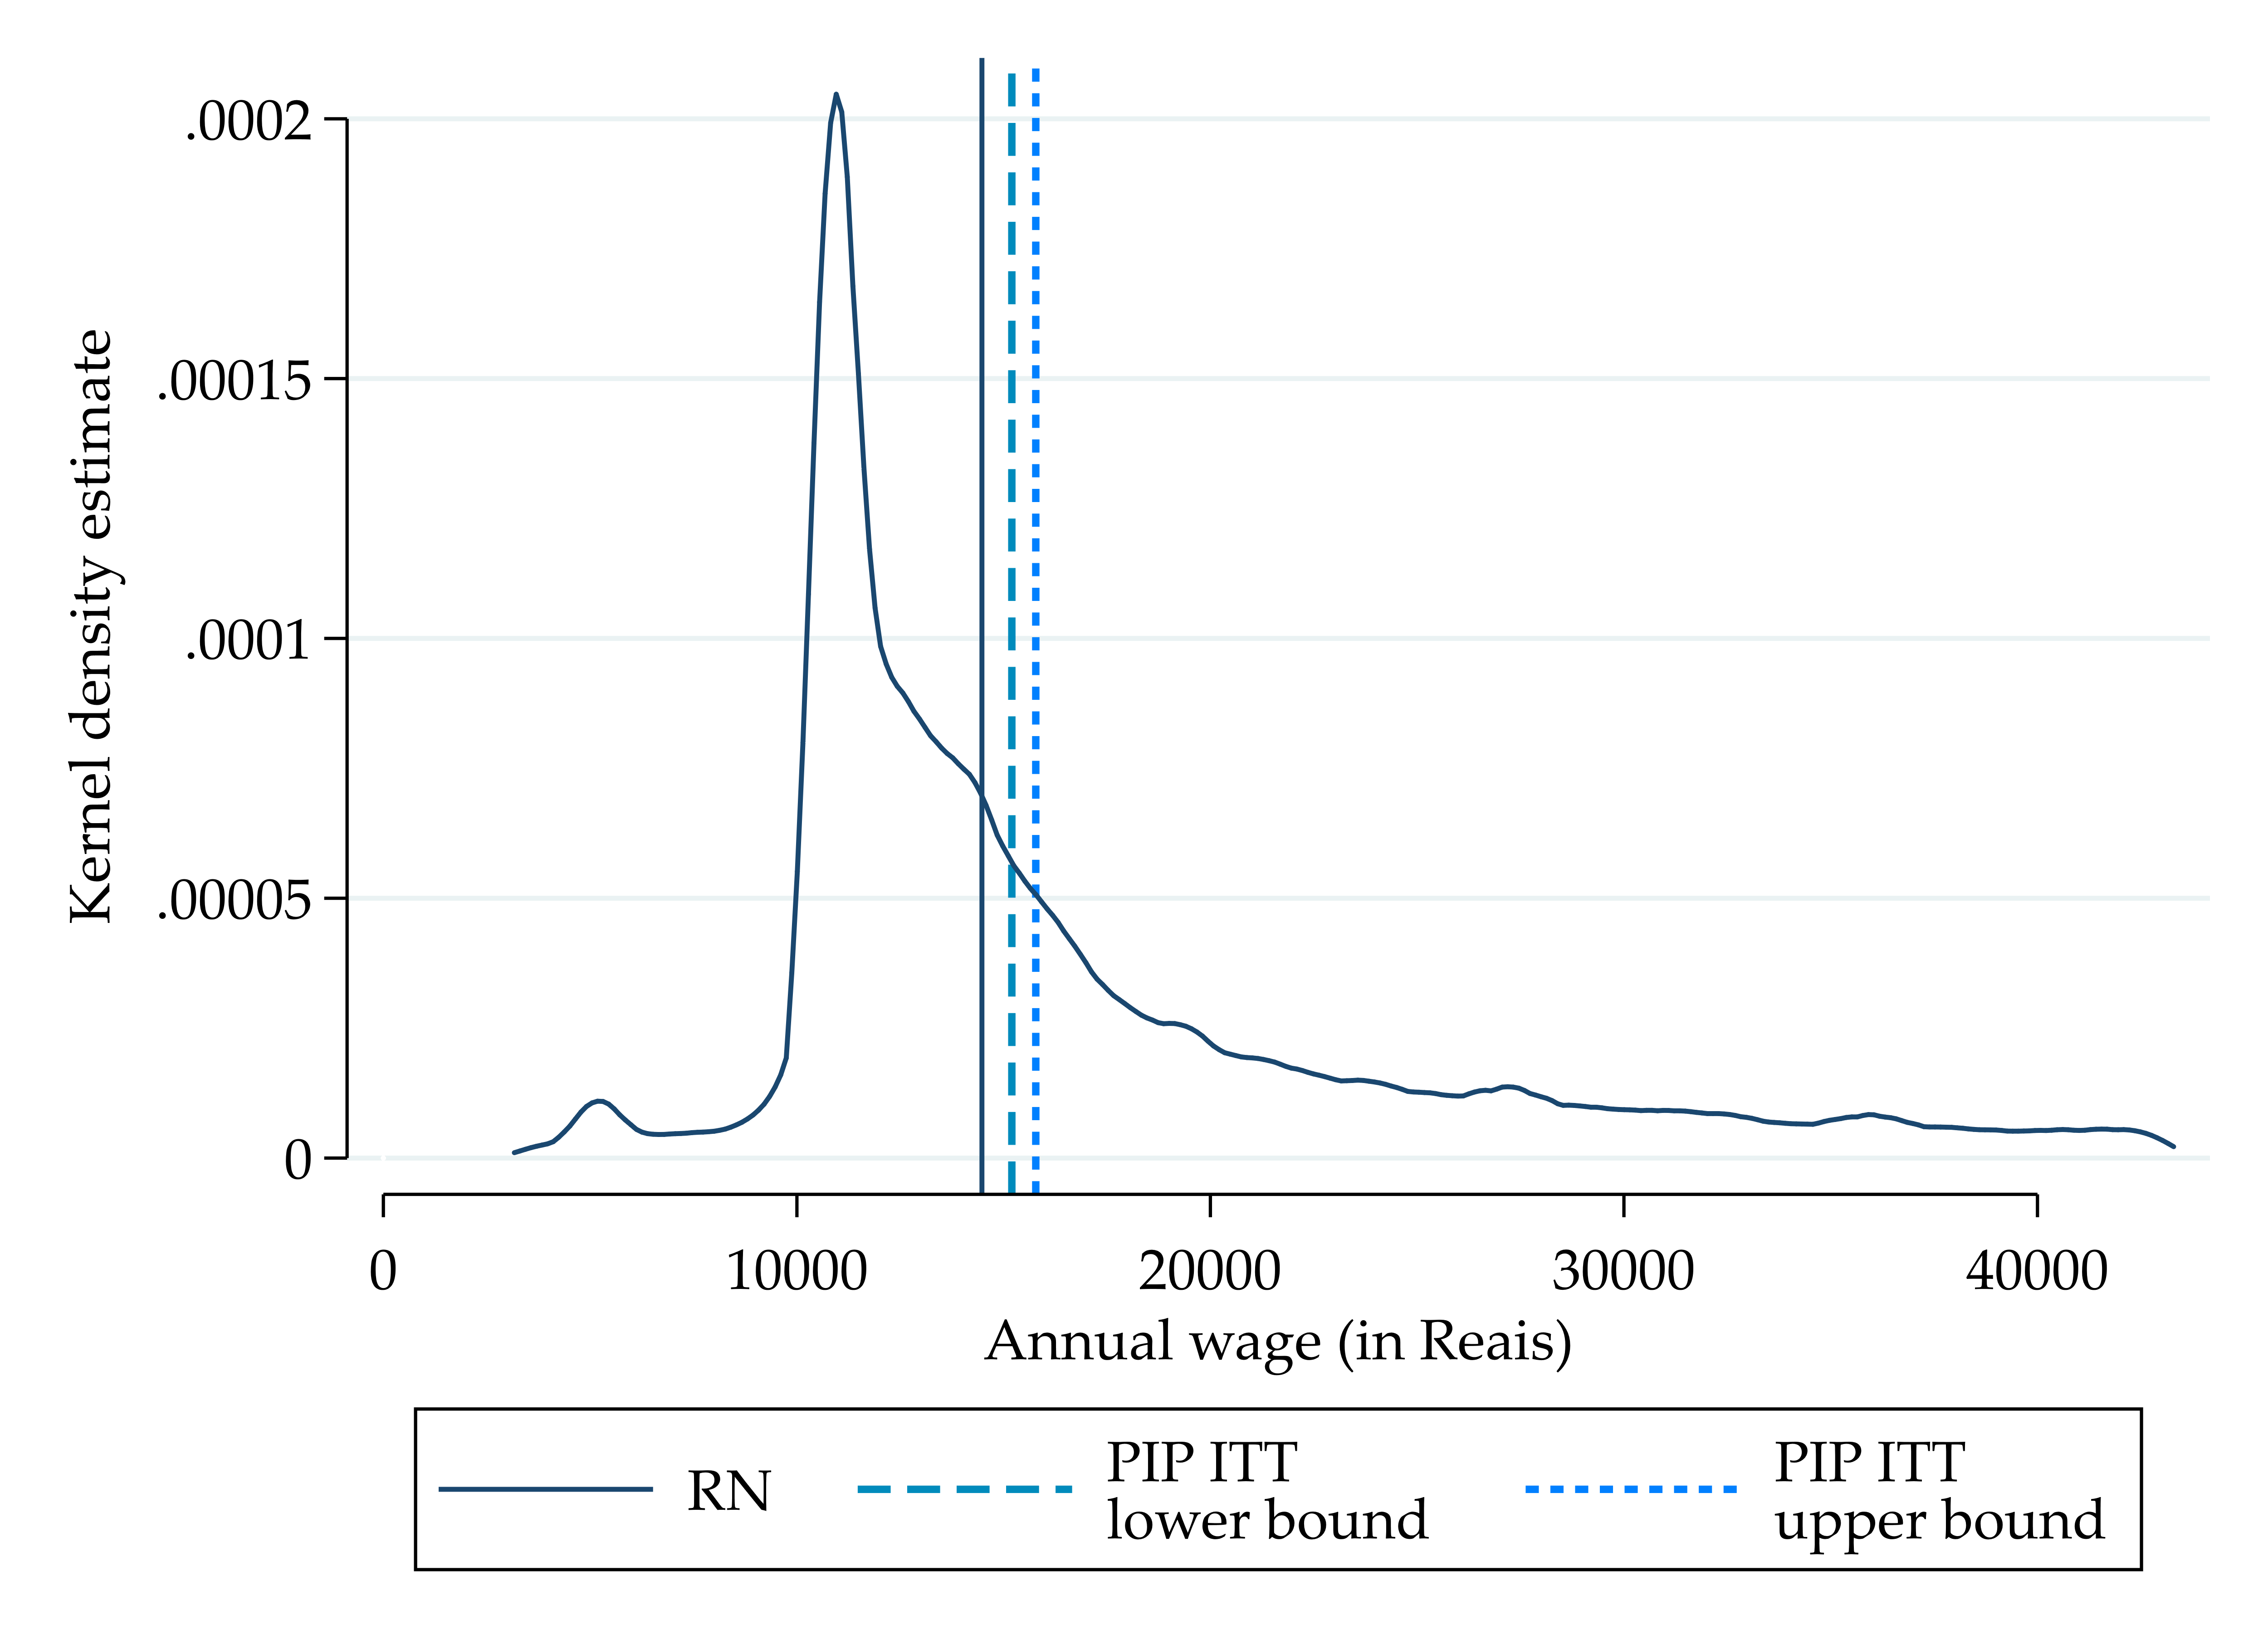
\includegraphics[width=14cm]{DataWork/Output/Figures/figB1-kdensity_wage.png}
		\label{fig:kdensity_wage}
		
		\begin{minipage}{0.825\textwidth}
			\small{\textit{Notes:} Kernel densities are computed using Epanechnikov kernel function. The three horizontal lines represent the median wage of Rio Grande do Norte (RN), which is considered as counterfactual, and of the median PIP student, assuming the effects on equivalent years of education estimated in Section \ref{sec:results} through an OLS model. Data are from 2016 \textit{Relação Anual de Informações Sociais} (RAIS). N = 801,956.}
		\end{minipage}
	\end{figure}
	
	\end{document}